\documentclass[phd,tocprelim]{cornell}
\let\ifpdf\relax

%
% tocprelim option must be included to put the roman numeral pages in the
% table of contents
%
% The cornellheadings option will make headings completely consistent with
% guidelines.
%
% This sample document was originally provided by Blake Jacquot, and
% fixed up by Andrew Myers.
%
%Some possible packages to include
\usepackage{hyperref}

\usepackage{graphicx,pstricks}
\usepackage{graphics}
\usepackage{amsmath}
\usepackage{amssymb}
\usepackage{moreverb}
\usepackage{wrapfig}
\usepackage{epsfig}
\usepackage{subfigure}
\usepackage{hangcaption}
\usepackage{txfonts}
\usepackage{palatino}
\usepackage{epigraph}
\usepackage{dsfont}
\usepackage{xcolor}
\usepackage{booktabs}
\usepackage[numbers]{natbib}


\DeclareSymbolFont{extraup}{U}{zavm}{m}{n}
\DeclareMathSymbol{\varheart}{\mathalpha}{extraup}{86}

\DeclareMathOperator*{\argmin}{arg\,min}
\DeclareMathOperator*{\argmax}{arg\,max}

\newcommand{\etal}{\textit{et al}.}
\newcommand{\ie}{\textit{i}.\textit{e}.}
\newcommand{\eg}{\textit{e}.\textit{g}.}

%if you're having problems with overfull boxes, you may need to increase
%the tolerance to 9999
\tolerance=9999

\bibliographystyle{plain}
%\bibliographystyle{IEEEbib}

\newcommand{\robobrain}{RoboBrain}
\newtheorem{example}{\hspace*{-1em}\textbf{Example}}

\renewcommand{\caption}[1]{\singlespacing\hangcaption{#1}\normalspacing}
\renewcommand{\topfraction}{0.85}
\renewcommand{\textfraction}{0.1}
\renewcommand{\floatpagefraction}{0.75}

%\title {Learning to represent unstructured large-scale visual data for robot perception}
%\title {Learning representations from unstructured large-scale visual data}
\title {Learning to represent large-scale visual data for robot perception}


\author {Ozan \c{S}ener}
\conferraldate {December}{2016}
\degreefield {Ph.D.}
\copyrightholder{Ozan \c{S}ener}
\copyrightyear{2016}

\graphicspath{{./images/},{./papers/ijcv/images/},{./Image/}}


\begin{document}

\maketitle
\makecopyright

\begin{abstract}
Your abstract goes here. Make sure it sits inside the brackets. If not,
your biosketch page may not be roman numeral iii, as required by the
graduate school.
\end{abstract}

\begin{biosketch}
Your biosketch goes here. Make sure it sits inside
the brackets.
\end{biosketch}

\begin{dedication}
To the Woodstock and the musicians of 60s.
\end{dedication}

\begin{acknowledgements}
%\epigraph{``I almost wish I hadn't gone down that rabbit-hole, and yet it's rather curious, you know, this sort of life!''}{\textit{Lewis Carroll\\ Alice's Adventures in Wonderland}}

\noindent \textbf{1 - Tale of the White Rabbit \cite{tale}}

\noindent ---~ \textbf{Fox:} ``What are you working on?''

\noindent ---~ \textbf{Rabbit:} ``My thesis.''

\noindent ---~ \textbf{Fox:} ``Hmmm. What's it about?''

\noindent ---~ \textbf{Rabbit:} ``Oh, I'm writing about how rabbits eat foxes''

\noindent ---~ \textbf{Fox:} ``That's ridiculous! Any fool knows that rabbits don't eat foxes''

\noindent ---~ \textbf{Rabbit:} ``Sure they do, and I can prove it. Come with me.''

They both disappear into the rabbit's burrow. After a few minutes, the rabbit returns, alone, to his typewriter and resumes typing.

\textbf{Scene inside the rabbit's burrow:} In one corner, there is a pile of fox bones. On the other side of the room, a huge lion is belching and picking his teeth. It doesn't matter what you choose for a thesis subject. It doesn't matter what you use for data. What does matter is who you have for a thesis advisor.

Following the tale of the white rabbit, I was advised by Ashutosh Saxena and He was flanked by Silvio Savarese. I am grateful to both of them for their scientific contribution, as well as allowing me to pursue my own ideas and patiently supporting me during the process. I am also thankful to my thesis committee members Emin G\"{u}n Sirer and David Mimno for their useful comments and suggestions. 

\noindent \textbf{2 - Down the Rabbit Hole @ Cornell}
First of all, I am grateful to Cornell Robot Learning Lab for creating a productive and fun environment both in Cornell and Stanford. I would like to thank Ashesh Jain, Dipendra Misra and Jae Sung for all the discussions and fun we had, Hema Koppula for all the guidance and help, and Ian Lenz and Chenxia Wu for their support and friendship.

I am thankful to everyone who made me feel like at home in New York State. Especially, members of red tigers trivia team Ken Yancey, Breana Branham and Sean Rice, my juggling and magic partner Tayyar Rezayev, the Cornell Tech crew Stephanie Hyland, Neel Madhukar, Faisal Alquaddoomi and Natalie Davidson, and last but not least Turks of Cornell: Sinem Unal and Melik Turker.

\begin{wrapfigure}{r}{0.25\textwidth}
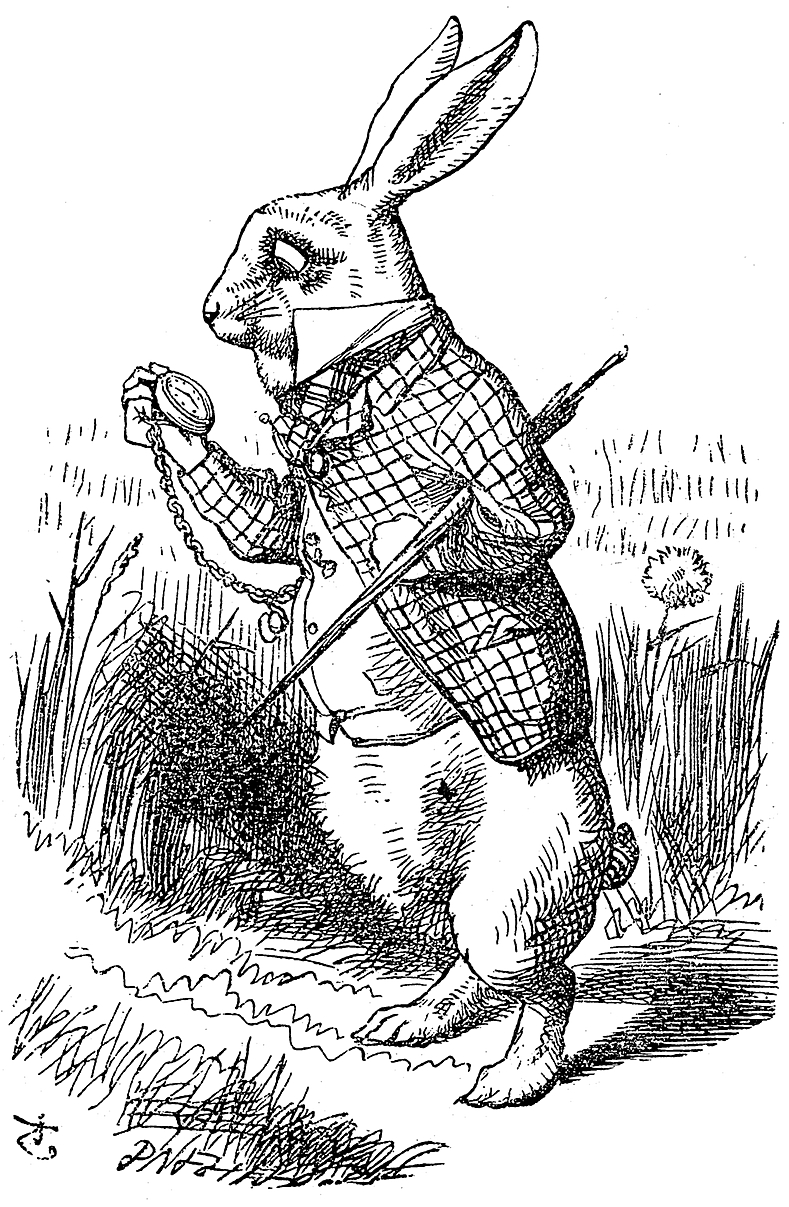
\includegraphics[width=0.24\textwidth]{alice.png}
\caption{The White Rabbit \cite{aiw}}
\end{wrapfigure}

\noindent \textbf{3 - A Mad Tea-Party @ Stanford}
I am grateful to Amir Zamir for countless impromptu discussions about life and science, and his guidance and help, Hyun Oh Song for his help in formalizing my ideas and Iro Armeni for her patience and understanding during our collaboration. I also had a chance to mentor two amazing undergrads during my PhD Hope Casey Allen and Jay Hack. I learned a lot from our discussions and hope to same for them. I am also grateful to all members of CVGL for their friendship, Alex, Amir, Yu, Chris, Kevin and Kuang. I am also grateful to Hakan Inan for all the discussions we had about random math topics. 

I am also thankful to everyone who converted this mad tea-party of silicon valley into a joyful experience. Ilbey, Saumitro, Jonathan Ho, Shane and Rebecca; thanks a lot for your friendship. Finally, I am also grateful to one of the most beautiful places in the world -Dolores Park-

\noindent \textbf{4 - Queen of Hearts $\varheart$}
It is rather tautological to say that I would not be the person who I am without my family. I thank my parents Omer and Gullizar as well as my brother Umut for their years of love and faith in me. 
% Zehra, Mom, Dad, Umut
\iffalse
\noindent ---~ \textbf{Lion:} ``Hello, Fox. Why are you looking so gloomy?''

\noindent ---~ \textbf{Fox:} ``It's been like this all week. First my cub got sick, then the car started making a funny noise, and last night I accidently put my watch through the washing machine and it quit working.''

\noindent ---~ \textbf{Lion:} ``Well, I can't do much about the child or the car, but I can fix your watch for you.''

\noindent ---~ \textbf{Fox:} ``That'll be the day. You with your big claws? You would have trouble picking up the watch, let alone fixing the insides. You'll just break it even worse than it already is. I'd better take it into town.''

\noindent ---~ \textbf{Lion:} ``Let me take it into my den for a couple minutes. You'll be suprized.''

So he disappears into his den with the watch. A few minutes later he returns: the watch is fixed.

\textbf{Scene inside the lion's den:} In one corner, next to the coffee machine, is a smug-looking lion lying on a couch cleaning his fur. In a second corner, there are seven industrious rabbits surrounded by tiny parts and precision tools.  It doesn't matter whether you can write working programs or prove theorems. It doesn't matter whether you can do a slick demo or generate pretty pictures. What really matters is whether your graduate students can.
\fi 

\end{acknowledgements}

\contentspage
\tablelistpage
\figurelistpage

\normalspacing \setcounter{page}{1} \pagenumbering{arabic}
\pagestyle{cornell} \addtolength{\parskip}{0.5\baselineskip}

\chapter{Introduction}
\epigraph{Either the locks were too large, or the key was too small.}{\textit{Lewis Carroll\\ Alice's Adventures in Wonderland}}
% !TEX root = ../../ozan_sener_thesis.tex
\label{intro}
Understanding  human activities is an important skill for robots working with humans. Robots not only need to detect the activity that human is performing but also need to anticipate \emph{what activity can a human possibly perform in the near future} in order to choose the right actions. Anticipation ability is especially important for assistive robots, and we have recently seen many successful collaborative robotics applications \cite{collob1,collob2,hemaISER} using the most likely action(s) humans might take in near future.
The set of the future possibilities is quite large, and robots need to be aware of all of them in addition to the most likely one. In this work, we focus on estimating the set of all possible future states with their likelihoods.

%For example, Koppula et al. \cite{hemaAnt} used anticipation in assistive robotic setting and successfully \emph{opened doors} and \emph{served drinks} by reacting to possible future human actions.

Anticipation is a challenging task, and it requires us to model the relationships between several objects and the human(s) in the scene, as well as their temporal evolution. Although the modelling assumptions and model parametrization varies, the common approach \cite{hemaAnt,gpcrf,hemaECCV,tian} is using Conditional Random Field (CRF) to represent the rich relations in the scene, and anticipating a single or a few most likely future states. Since the future is ambiguous, the most likely state might not be sufficient enough to assess the risk of each action. For example, consider a collaborative cooking scenario, the object that human is reaching is typically a distribution over many objects. Computing the trajectory, that is least likely to conflict with the human, is only possible via consideration of all future possibilities. The question, we address in this chapter, is: \emph{How can we estimate all plausible future activities and their probabilities in a scene modelled by a CRF?}

%Moreover, we call these probabilities as a \emph{belief}.
%Since we focus on finding all plausible future actions and their respective probabilities, we study the limitations of CRFs in such a setting
%A standard approach for anticipating future human activities is modelling the rich relationships in the scene by using Conditional Random Fields (CRFs). Moreover,
%Moreover, detecting the activity human is performing
%not only needs to understand the activity a human is performing, but also need to perform reactive responses.
%Consider the applications of surveillance and  robotics, where given an input video, one
 %For example, an alert may need to be issued in the case of surveillance or a reactive action may need to be taken by a robot in the case of co-robot scenario.
%Anticipation of the possible human activities is a challenging task and it require us to model the


% A standard approach is to use a Conditional Random Field (CRF) to represent the relations between the objects, human(s) and activities \cite{hemaIJRR,hemaAnt}.  %In general, it is possible to obtain the maximum a posteriori (MAP) solution over a CRF to find most likely future action(s).

 %However, a robot needs more than the most likely state(s) in order to make a decision. Robot needs all plausible futures with their corresponding belief values. For example, a plausible but less likely future might require taking precautions like getting close enough to react.



%A recent work \cite{embr,divmbest}, empirically computes modes of the CRF likelihood by relying on diverse samples. While this work does not apply directly to estimating beliefs in a Bayesian filtering setting,  We use the diverse sampling ideas for efficient inference in our model (see Section~\ref{relwork} for more details).

\begin{figure}[t]
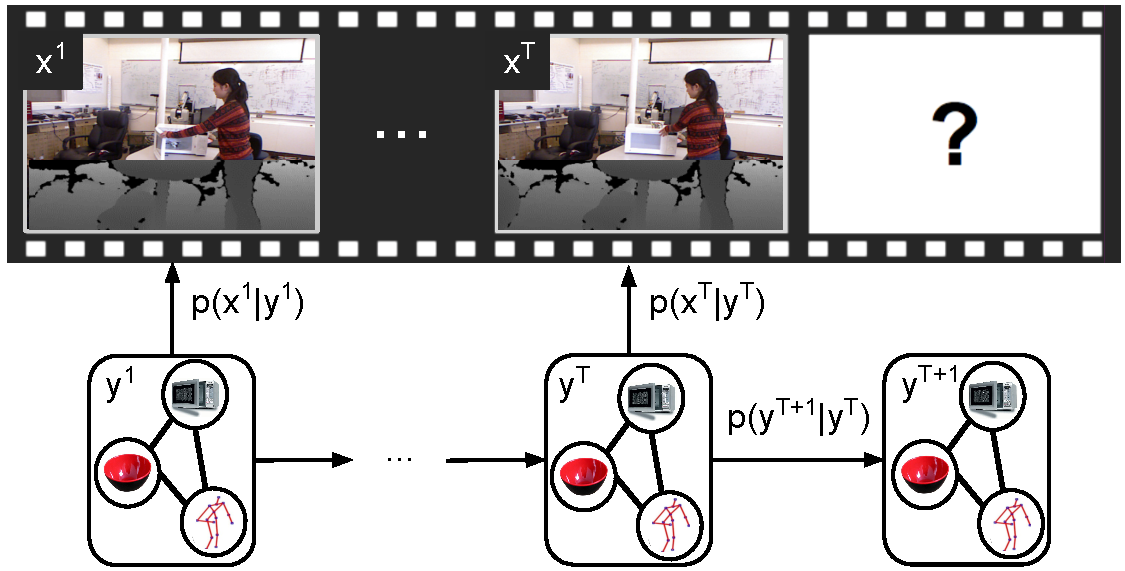
\includegraphics[width=\textwidth]{Fig1}
\caption{Figure is showing the state and measurements at each time represented by a CRF.
Our algorithm, rCRF, enables the application of recursive Bayesian estimation to CRF-based scene models. rCRF computes the full belief over human activity and object affordances ($y^1,\ldots,y^{T+M}$) by using RGB-D Video ($x^1,\ldots,x^T$).}
% In order to so, we propose a new model, rCRF, which can jointly use bayesian filtering and CRFs.}
%  which are not observed.}
%Estimating the belief over a CRF and using the estimated belief for anticipation and robot planning. \emph{(Colors of the nodes are representing the labels.)}}
\label{fig1}
\end{figure}

% modeling temporal evolution is still challenging in such a setting since the sampling procedure does not use temporal information \emph{(see Section~\ref{relwork} for mote details on this challenge)}.
Bayesian filtering methods can accurately estimate a belief (set of probabilities) over variables of interest from sequential data. However, it is still very challenging to estimate a belief over a CRF for two reasons. Firstly, it is not tractable to enumerate the labels over a CRF model since the output space has a dimension exponential in the number of objects, labels, and the temporal length\footnote{Typically with 10 objects, 10 min. length (with 1 sec. long segments), 10 activity and 10 object labels, dimension is $(10^{10}\times10)^{10\times60}=10^{6600}$.}. Secondly, there is a modelling difference between CRFs and Bayesian filtering framework. CRF is based on a discriminative setting whereas the Bayesian filtering mostly relies on the generative formulation.
% that requires the conditional probability of the observation given the variables of interest.
%where it models the conditional probability of the variables of interest given an observation,

In this chapter, we present a recursive algorithm -- Recursive CRF (rCRF) -- which can efficiently estimate a full belief over a CRF-based temporal scene model. rCRF can be seen as an efficient belief estimation method which enables us to use CRF-based scene model in Bayesian filtering. It models the temporal evolution via Bayesian updates and models the measurements in the scene via CRF. In order to use CRFs in such a scenario, we solve two problems. First, we present an approximation to convert the discriminative likelihood of the CRF into a generative measurement equation. Second, we use structured diversity for tractable computation. To the best of our knowledge, rCRF is the only tractable method that can use a CRF-based scene model in a recursive Bayesian filtering.
%Since we define the belief function recursively, we iterate the message propagation and diverse sampling until the convergence.

We apply the rCRF to the problem of activity detection and anticipation from RGB-D data. As a CRF-based scene model, we use the model from \cite{hemaIJRR} which represents the scene as a CRF over human activity and object affordances. We then use the RGB-D video to detect and anticipate activities via rCRF. %We use the rCRF framework in order to anticipate the future activities as well.

Our experiments show that we outperform the state-of-the-art methods for detection and anticipation, and the improvement in the anticipation accuracy is significant. In addition to the improvements in accuracy, we show that our anticipation also improves the computation time and runs near real-time.

%We believe that the presented efficient and accurate estimation of a full belief can be combined with an optimal decision mechanisms (e.g. minimum Bayes risk \cite{decisionTheory,nabbe2007extending}) for better assitive robots.

In summary, the contributions of this work are:
\begin{itemize}
\item  We present Recursive-CRF (rCRF) method that uses the rich modeling power of CRF in
Bayesian filtering setting.
%  allows CRF-based scene models in a Bayesian filtering.
% \item  We present a recursive method in order to estimate the full belief over an rCRF.
\item  We present a structured-diversity based approach to enable tractable computation of the belief.
\item  We apply our rCRF method to the problem of activity detection and anticipation in
RGB-D videos.
%\item  Our experiments show that rCRF significantly outperforms the state-of-the-art methods, both in accuracy and inference time.
\end{itemize}


\chapter{Sensing at Scale - RoboBrain}
\epigraph{Parents of young organic life forms should be warned, that towels can be harmful, if swallowed in large quantities.}{\textit{Douglas Adams\\ Hitchhiker's Guide to the Galaxy}}
% !TEX root = ozan_sener_thesis.tex

Robotics systems are typically composed of many sub-systems and these systems are developed in isolation. Moreover, robots learn continuously after deployment using human feedback is isolation as well. Hence, one of the most critical problems in robotics is sharing knowledge among different robotic systems as well as robotics sub-systems in deployement. In this chapter, we introduce the knowledge-engine we developed which enables robotics systems to share knowledge among robotic platforms as well as robotics sub-systems. The knowledge-engine we developed can handle variety of modalities and domains. More importantly, the knowledge comes from a variety of sources including online knowledge bases, learned concepts from robotics research groups from all over the world as well as physical robotic experiments.

\noindent\textbf{Contributions of this chapter.} We developed this knowledge engine in collaboration with Saxena, Jain, Jami, Misra and Koppula, and we call it RoboBrain. Within the scope of this dissertation, I contributed to a large-scale distributed system architecture which can scale to thousands of videos, images and text files. For completeness, in this chapter we also describe the formal definition of knowledge-engine, the query language for accessing the knowledge and a various applications of RoboBrain. RoboBrain is available at: http://www.robobrain.me



% !TEX root = ../../ozan_sener_thesis.tex
% \vskip .1in
\section{Why do we need robot knowledge bases?}
Over the last decade, we have seen many successful applications of large-scale knowledge systems.
%  many inclusive web services have been developed  by successfully combining information at a large-scale.
Examples include  Google knowledge graph \cite{dong2014knowledge}, IBM Watson~\cite{ferrucci2010}, Wikipedia,
 and many others.
These systems know answers to many of our day-to-day questions, and
 not crafted for a specific task, which makes them valuable for humans.
Inspired by them, researchers have aggregated domain specific knowledge by mining
data~\cite{dbpedia2007, freebase2008}, and processing natural
language~\cite{nell2010}, images~\cite{imagenet2009} and
speech~\citep{mohamed2011deep}.  These sources of knowledge are specifically designed for humans, and their  human centric design makes them of limited use for robots---for example, imagine a robot querying a search engine
 for how to ``bring sweet tea from the kitchen" (Figure~\ref{fig:intro}).


 %Contrary to humans, for whom incomplete and ambiguous instructions may suffice,
 In order to perform a task, robots require access to a large variety of information with finer details for performing
 perception, planning, control and natural language understanding. When asked to bring sweet tea, as shown in Figure~\ref{fig:intro}, the robot
 would need access to the knowledge for grounding the language symbols into physical entities,
  the knowledge that sweet tea can either be on a table or in a fridge, and the knowledge for inferring the
 appropriate plans for grasping and manipulating objects. Efficiently handling this joint knowledge representation across different
 tasks and modalities is still an open problem.

In this chapter we present \robobrain{} that allows robots to learn and share such representations of knowledge.
We learn these knowledge representations from a variety of sources, including interactions that robots have while performing perception,
planning and control, as well as natural language and visual data from the Internet.
Our representation considers several modalities including symbols, natural language, visual or shape features, haptic properties, and so on. \robobrain{} connects this knowledge from various sources and allow robots to perform diverse tasks by jointly reasoning over multiple data modalities.  %Moreover, our experiments suggest that by connecting different modalities and projects, robots can share knowledge and collectively improve their abilities.

 \begin{figure}
 \centering
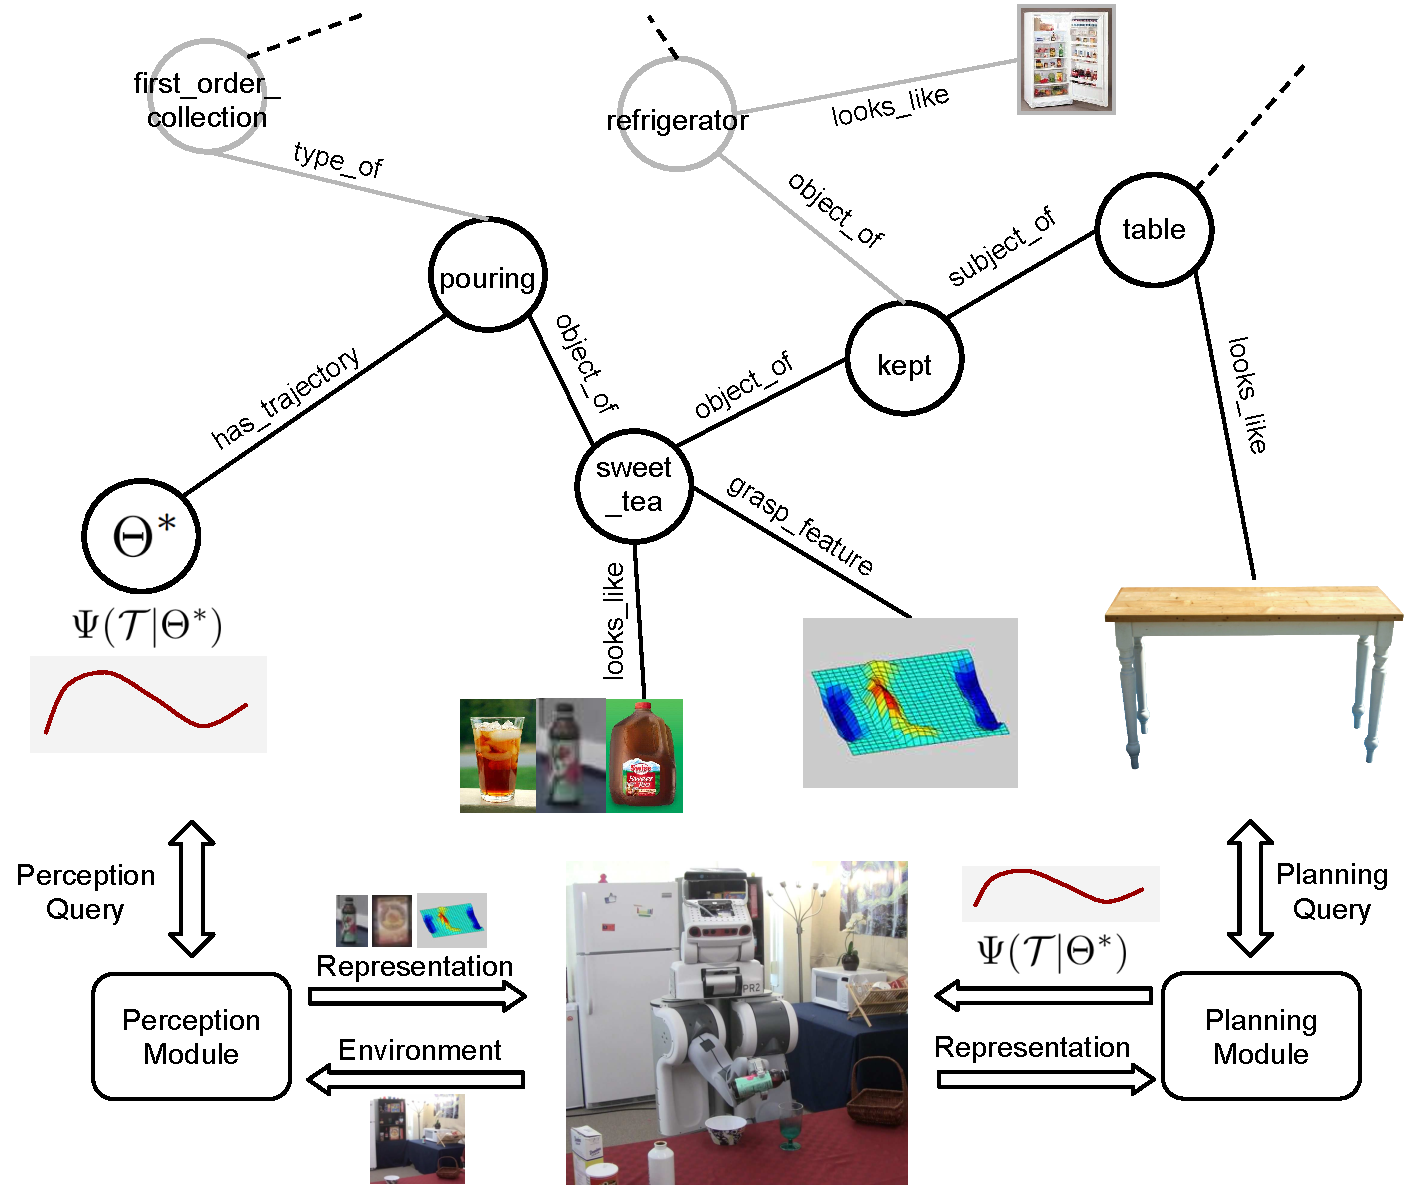
\includegraphics[width=\linewidth]{Image/cover_picture_graph}
 \caption{\textbf{An example showing a robot using \robobrain{} for performing tasks.}  The robot is asked ``Bring me sweet tea from the kitchen", where
 it needs to translate the instruction into the perceived state of the environment.
\robobrain{} provides useful knowledge to the robot for performing the task:
 (a) sweet tea can be kept on a table or inside a refrigerator,
 (b) bottle can be grasped in certain ways,
 (c) opened sweet tea bottle needs to be kept upright,
 (d) the pouring trajectory should obey user preferences of moving slowly to pour, and
 so on.
 }
 \label{fig:intro}
 \end{figure}

\begin{figure*}[t]
\centering
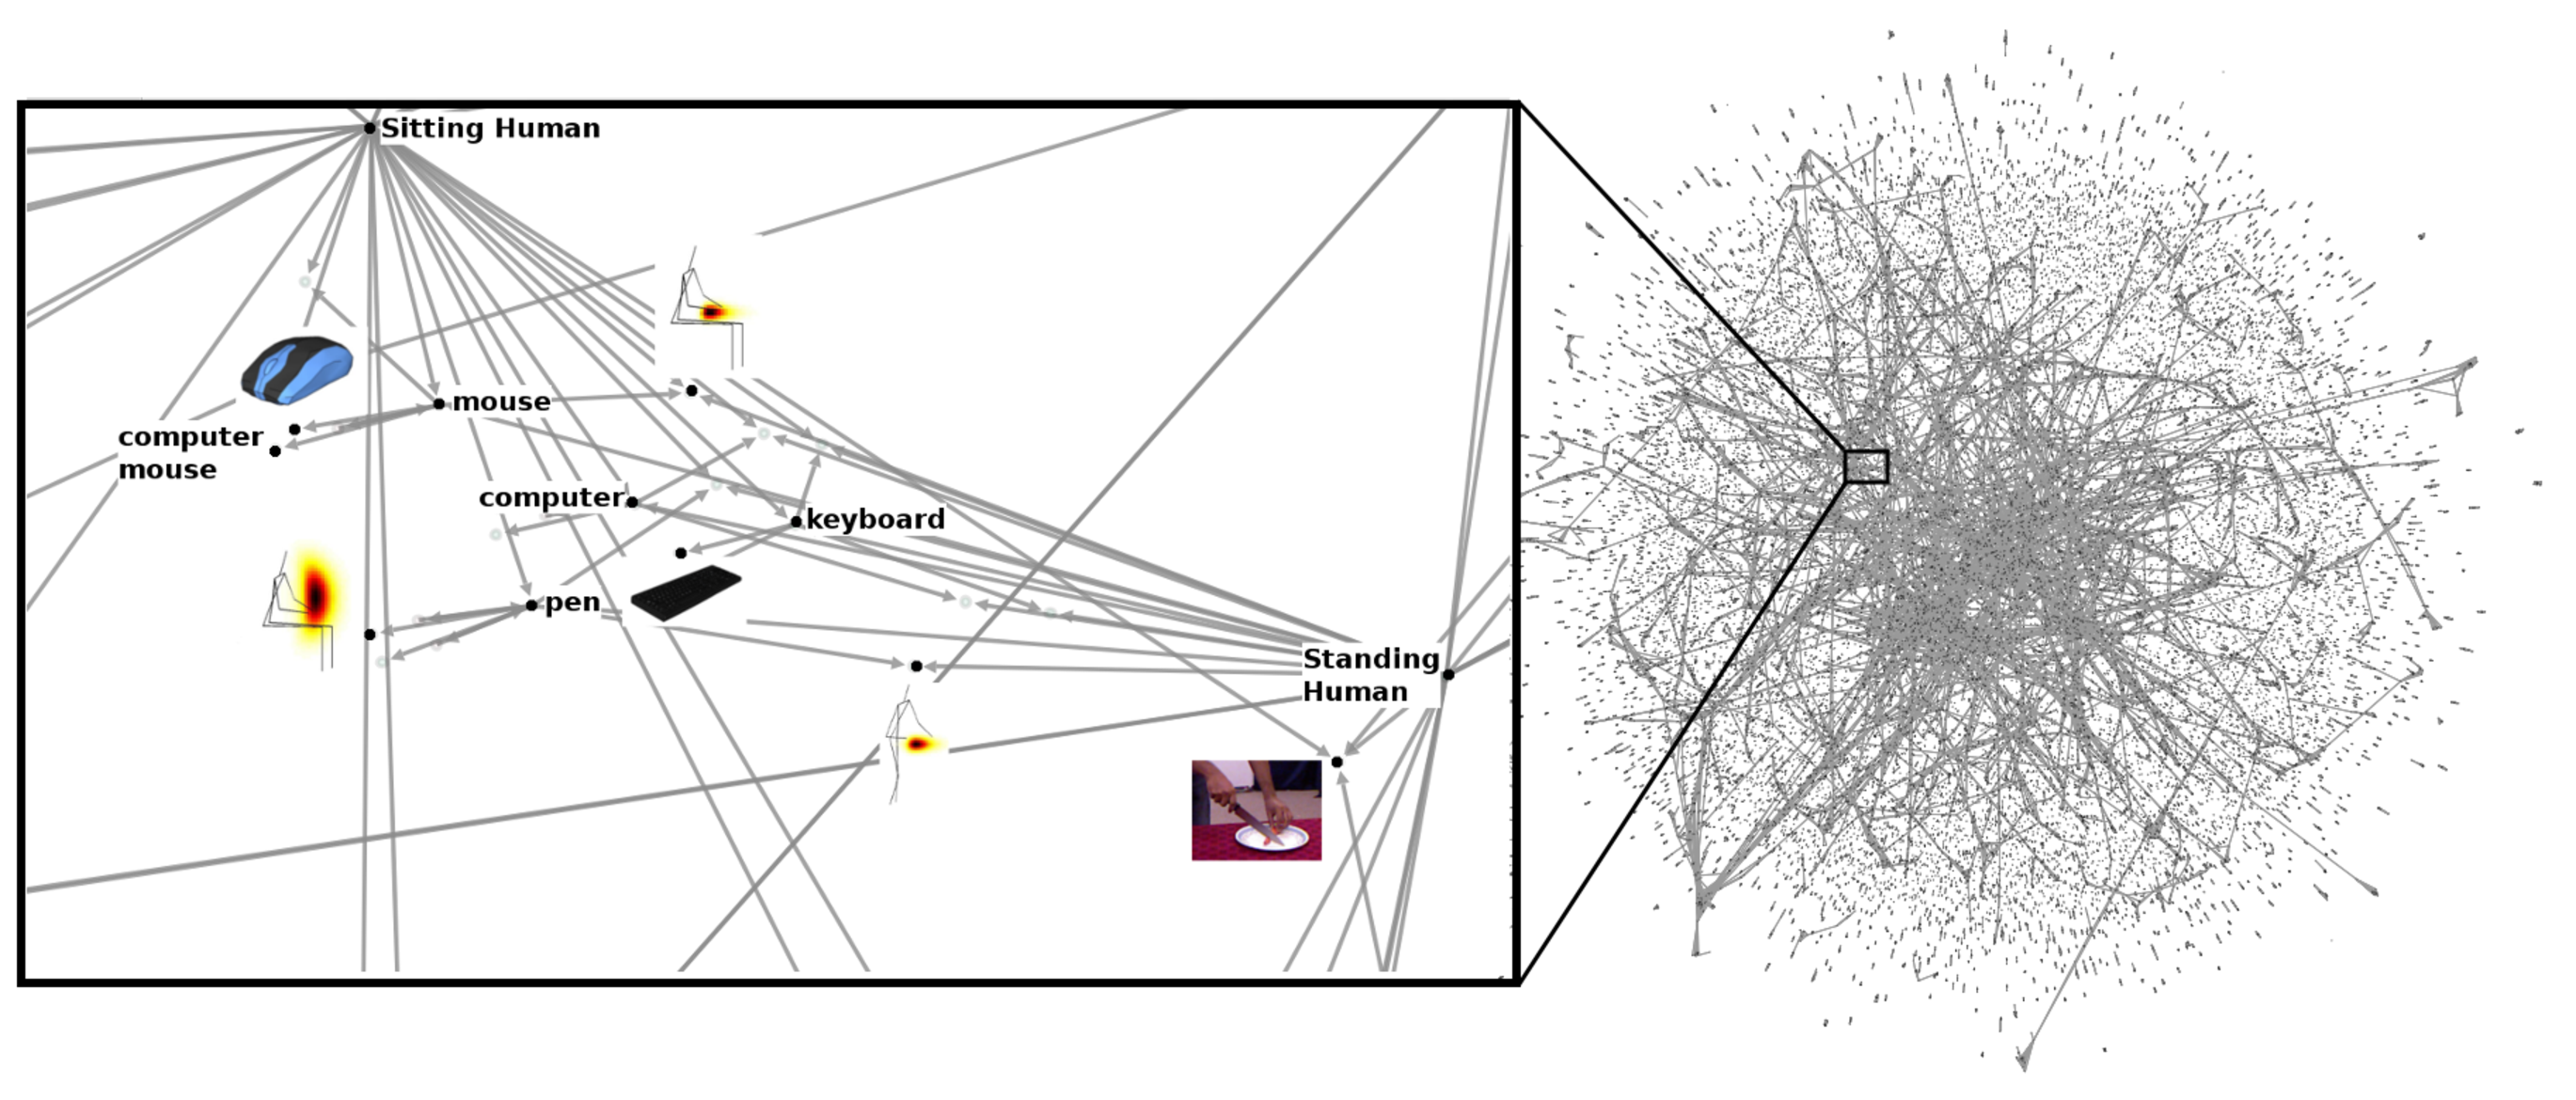
\includegraphics[width=.95\linewidth, height=2.6in, clip=true, trim=0 40 0 0]{Image/RBgraph}
\caption{\textbf{A visualization of the \robobrain{} graph} on Nov 2014, showing about 45K nodes and 100K directed edges.
%  from the RoboBrain's knowledge graph.
The left inset shows a zoomed-in view of a small region of the graph with rendered media. This illustrates the relations between multiple modalities namely images, heatmaps, words and human poses. \textit{For high-definition graph visualization, see: \url{https://sites.google.com/site/robotknowledgeengine/}}}
\label{fig:graph}
\end{figure*}


\robobrain{} enables sharing from multiple sources by representing the knowledge in a graph structure.
% RKE enables knowledge sharing by representing the knowledge in a graph representation.
% Thcontaining
% out of the
% information that robots need for performing various tasks.
%Knowledge in  RKE comes from multiple sources, which is integrated into the graph structure of RKE.
Traversals on the \robobrain{} graph allow robots to gather the specific information they need for a task. This includes the  semantic information, such as different grasps of the same object, as well as the functional knowledge, such as spatial constraints (e.g., a bottle is kept on the table and not the other way around).
The key challenge lies in building this graph from a variety of knowledge sources while ensuring dense connectivity across nodes. Furthermore, there are several  challenges in building a system that allows concurrent and distributed update, and retrieval operations.

We  present use of \robobrain{} on three robotics applications in the area of grounding natural language, perception and planning.
For each application we show usage of \robobrain{} \textit{as-a-service}, which allow researchers to effortlessly use the state-of-the-art algorithms. We also present experiments to show that sharing knowledge representations through \robobrain{} improves existing language grounding and path planning algorithms.


\robobrain{} is a collaborative project that we support by designing a large-scale cloud architecture.
%and we designed a large-scaled cloud architecture to enable this collaboration efficiently.
In the current state, \robobrain{} stores and shares knowledge across several research projects~\cite{tellex2011understanding,misra2014tell,jainsaxena2013_trajectorypreferences,jiang-hallucinatinghumans-labeling3dscenes-cvpr2013,jiang2012humancontext,KoppulaRSS2013,wulenzsaxena2014_hierarchicalrgbdlabeling,lenz2013_deeplearning_roboticgrasp} and Internet knowledge sources~\citep{cyc1995,wordnet1998}.
% RKE has knowledge from \cite{misra2014tell,tellex2011understanding,jainsaxena2013_trajectorypreferences,jiang-hallucinatinghumans-labeling3dscenes-cvpr2013}.
We believe as more research projects contribute knowledge to \robobrain{}, it will not only improve the concerned project but will
also be beneficial for the robotics community at large.
%their robots perform better but we also believe this will be beneficial for the robotics community at large.
%The RKE is under open Creative Commons Attribution license\footnote{http://creativecommons.org/licenses/by/2.5, Extra conditions may apply depending on the data sources, see anonymous.me for detailed information.} and is
%avalable at: \texttt{\url{http://anonymous}}

The goal of the chapter is to present an overall view of the \robobrain{}, its architecture, functionalities, and demonstrate its application to robotics. In Section~\ref{sec:graph} we formally define the \robobrain{} graph and describe its
system architecture in Section~\ref{sec:system}. In order for robots to use
\robobrain{} we propose the Robot Query Library in Section~\ref{sec:raquel}. In
Section~\ref{sec:applications} we present different robotic applications using \robobrain{}.


% !TEX root = ../../ozan_sener_thesis.tex
\section{Related Work on Robot Knowledge Bases}
\label{sec:relatedwork}
We now describe some works related to \robobrain{}. We first give an overview of the existing knowledge bases and describe how \robobrain{} differs from them. We then describe some works in robotics that can benefit from \robobrain{}, and also discuss some of the related on-going efforts.

\smallskip

% !TEX root = robobrain.tex
\noindent
\textbf{Knowledge bases.}
Collecting and representing a large amount of information in a knowledge base (KB) has been widely studied in the
areas of data mining, natural language processing and machine learning. Early seminal works have manually created KBs for the study of common sense knowledge (Cyc \cite{cyc1995}) and lexical knowledge (WordNet \cite{wordnet1998}). With the growth of Wikipedia, KBs started to use crowd-sourcing (DBPedia \cite{dbpedia2007}, Freebase \cite{freebase2008}) and automatic information extraction (Yago \cite{yago2007,yago22013}, NELL \cite{nell2010}) for mining knowledge.

One of the limitations of these KBs is their strong dependence on a single modality that is the text modality. There have been few successful attempts to combine multiple modalities. ImageNet \cite{imagenet2009} and NEIL \cite{chen_iccv13} enriched text with images obtained from Internet search. They used crowd-sourcing and unsupervised learning to get the object labels. These object labels were further extended to object affordances \cite{zhu2014}.

We have seen successful applications of the existing KBs within the modalities they covered, such as IBM Watson Jeopardy Challenge \cite{ferrucci2012a}. However, the existing KBs are human centric and do not directly apply to robotics. The robots need finer details about the physical world, e.g., how to manipulate objects, how to move in an environment, etc. In \robobrain{} we combine knowledge from the Internet sources with finer details about the physical world, from \robobrain{} project partners, to get an overall rich graph representation.

\smallskip


% !TEX root = robobrain.tex


\noindent
\textbf{Robot Learning.}
For robots to operate autonomously they should perceive their environments, plan paths, manipulate objects and interact with humans. We describe previous work in each of these areas and how \robobrain{} complements them.

\noindent
\emph{Perceiving the environment.} Perception is a key element of many robotic tasks. It has been applied to object labeling~\cite{lai:icra11a, KoppulaIJRR2012,wulenzsaxena2014_hierarchicalrgbdlabeling}, scene understanding~\cite{KitaniECCV2012,guptaECCV14}, robot localization~\cite{McManus-RSS-14,NaseerAAAI14},  path planning~\cite{KatzAR14}, and object affordances~\cite{delaitre2012, KoppulaECCV14}. \robobrain{} stores perception related knowledge in the form of 3D point clouds, grasping features, images and videos. It also connects this knowledge to human understandable concepts from the Internet knowledge sources.



\noindent
\emph{Path planning and manipulation.} Planning algorithms formulate action plans which are used by robots to move around and modify its environment. Planning algorithms have been proposed for the problems of motion planning~\cite{ZuckerCHOMP13, SchulmanRSS13},  task planning~\cite{alami2006toward, BolliniISER12} and symbolic planning~\cite{edelkamp2009optimal, rintanen2012planning}. Some planning applications include robots baking cookies~\cite{BolliniISER12}, folding towels~\cite{Maitin-ShepardICRA10}, assembling furniture~\cite{KnepperICRA13}, and preparing pancakes~\cite{Beetz11}. The previous works have also learned planning parameters using methods such as Inverse Optimal Control~\citep{AbbeelIJRR10,Ratliff06,ZiebartAAAI08,jainsaxena2013_trajectorypreferences}. \robobrain{} stores the planning parameters learned by previous works and allow the robots to query for the parameters.

\iffalse
\noindent
\emph{Path and manipulation planning.} There exist a large class of algorithms which allow
robots to move around and modify the environment. Broadly planning algorithms can be
categorized as motion planning \cite{ZuckerCHOMP13, SchulmanRSS13},
 task planning \cite{alami2006toward, BolliniISER12} and symbolic planning
 \cite{edelkamp2009optimal, rintanen2012planning}.
Bakebot \cite{BolliniISER12}, towel-folding \cite{Maitin-ShepardICRA10}, IkeaBot \cite{KnepperICRA13} and robots preparing pancakes \cite{Beetz11}
are few of the many successful planning applications.
Most planning algorithms abstract out the perception details, however access to
perception and manipulation knowledge can allow robots to plan in dynamic real world environments.
\fi


\noindent
\emph{Interacting with humans.} Human-robot interaction includes collaborative tasks between humans and robots~\cite{NikolaidisISR10,nikolaidis2013human}, generating safe and human-like robot motion~\cite{Mainprice13,LasotaCASE14,GielniakIJRR13,DraganRSS13,CakmakIROS11}, interaction through natural language~\cite{TellexRSS14,misra2014tell}, etc. These applications require joint treatment of perception, manipulation and natural language understanding. \robobrain{} stores different data modalities required by these applications.
\iffalse
\noindent
\emph{Interacting with humans.} Another important aspect is
human-robot interaction. Previous works have focused on various aspects,
such as human-robot collaboration for task completion \cite{NikolaidisISR10, koppula-anticipatoryplanning-iser2014}, generating safe
robot motion near humans \cite{Mainprice13, LasotaCASE14},
 obeying user preferences \cite{CakmakIROS11},
 generating human like and legible motions \cite{GielniakIJRR13, DraganRSS13},
interaction through natural language \cite{TellexRSS14,misra2014tell}, etc.
These applications require joint treatment of perception, manipulation and natural language understanding.

%All these applications require access to perception, manipulation, language understanding, etc.,
%further demonstrating the need for large scale multi-modal data.



%Although, there has been significant success in addressing these problems individually,
%previous works were not able to exploit the common information shared by these problems.
%For example, \todo{rewrite the example below and clarify why they couldnt use the shared information..
%However, these problems share many common information which previous works have not exploited.
%Such as previous works have perceived
%environments with cups, have manipulated with for pouring water and have learned
%how to manipulate it near human when it contains hot coffee. }
%Our RoboBrain knowledge engine enables sharing information across these tasks by allowing
%queries to the graph for information spanning several sub-problems.
\fi

Previous efforts on connecting robots range from creating a common operating system (ROS) for
 robots \cite{Quigley09}
to sharing data acquired by various robots via cloud \cite{RoboEarth, KIVA}.
For example, the RoboEarth \cite{RoboEarth} provides a platform for the robots to store and off-load computation
to the cloud and communicate with other robots; and the KIVA systems \cite{KIVA} use the cloud to coordinate motion for hundreds of mobile platforms. On the other hand, \robobrain{} provides a
knowledge representation layer on top of data storing, sharing and communication.

Open-Ease~\cite{openease} is a related on-going effort towards building a knowledge engine for robots.
Open-Ease and \robobrain{} differ in the way they learn and represent knowledge. In Open-Ease the knowledge is represented as formal statements using pre-defined templates. On the other hand, the knowledge in \robobrain{} is represented as a graph. The nodes of the \robobrain{} graph have no pre-defined templates and they can be any robotic concept like grasping features, trajectory parameters, and visual data. This graph representation allows partner projects to easily integrate their learned concepts in \robobrain{}. The semantic meaning of concepts in the \robobrain{} graph are represented by their connectivity patterns in the graph. %The Open-Ease is similar to the \robobrain{} in that it also collects knowledge through robot interactions.
\iffalse
A closely related on-going effort is Open-Ease \cite{openease}
It focuses on a similar problem of cloud knowledge-base and inference engine for robots.
It is different from \robobrain{} in a way it incorporates knowledge and do inference.
Open-ease requires input to be in the form of a facts written in a formal logic statements following the pre-defined structure and uses an
inference engine designed for the language. On the other hand, \robobrain{} accepts unstructured information as nodes and their relations as edges.
\robobrain{} automatically infers the structure and it also infers the correctness and the latent semantic meaning. Our approach brings flexibility with the cost
of a technical challenges in inference and learning.
\fi




% !TEX root = robobrain.tex

% \section{Technical Challenges}
\section{Overview}
\label{overviewPaper}

\robobrain{} is a never ending learning system  that  continuously incorporates
new knowledge from  its partner projects and from different Internet sources.
One of the functions of \robobrain{} is to represent the knowledge from various sources as a graph,
as shown in  Figure~\ref{fig:graph}. The nodes of the graph represent concepts and edges represent the
relations between them. The connectivity of the graph is increased through a set of graph operations
that allow additions, deletions and updates to the graph. As of the date of this submission,
\robobrain{} has successfully
connected knowledge from sources like WordNet, ImageNet, Freebase, OpenCyc,
 parts of Wikipedia and other partner projects. These knowledge sources provide lexical knowledge, grounding of concepts into images and common sense facts about the world.

The knowledge from the partner projects and Internet sources can sometimes be erroneous. \robobrain{}
handles inaccuracies in  knowledge by maintaining beliefs over the correctness of the concepts and
relations. These beliefs depend on how much \robobrain{} trusts a given source of knowledge, and also the
feedback it receives from crowd-sourcing (described below). For every incoming knowledge, \robobrain{}
also makes a sequence of decisions on whether to form new nodes, or edges, or both. Since the
knowledge carries semantic meaning \robobrain{} makes many of these decisions based on the
contextual information that it gathers from nearby nodes and edges. For example, \robobrain{} resolves
polysemy using the context associated with nodes. Resolving polysemy is important because a `plant'
could mean a `tree' or an `industrial plant' and merging the nodes together will create errors in the
graph.


\robobrain{} incorporates supervisory signals from humans in the form of crowd-sourcing feedback. This
feedback allows \robobrain{} to update its beliefs over the correctness of the knowledge, and to modify the
graph structure if required. While crowd-sourcing feedback was used in some previous works as
means for data collection (e.g.,~\citep{imagenet2009,Russell08}), in \robobrain{} they serve as supervisory
signals that improve the knowledge engine. \robobrain{} allows user interactions at multiple levels: (i)~
Coarse feedback: these are binary feedback where a user can ``Approve'' or ``Disapprove'' a concept
in \robobrain{} through its online web interface; (ii) Graph feedback: these feedback are elicited on 
\robobrain{} \textit{graph visualizer}, where a user modifies the graph by adding/deleting nodes or edges; (iii)
Robot feedback: these are the physical feedback given by users directly on the robot.

In this paper we discuss different aspects of \robobrain{}, and show how \robobrain{} serves as a knowledge layer for the robots. In order to support knowledge sharing, learning, and crowd-sourcing feedback we develop a large-scale distributed system. We describe the architecture of our  system in Section~\ref{sec:system}. In Section~\ref{sec:raquel} we describe the robot query library, which allow robots to interact with \robobrain{}.  Through experiments we show that robots can use \robobrain{} \textit{as-a-service} and that knowledge sharing through \robobrain{} improves existing robotic applications. We now present a formal definition of our Robot Knowledge Engine and the graph.



% !TEX root = robobrain.tex

\begin{figure}[t]
\centering
\subfigure[original graph]{\label{a}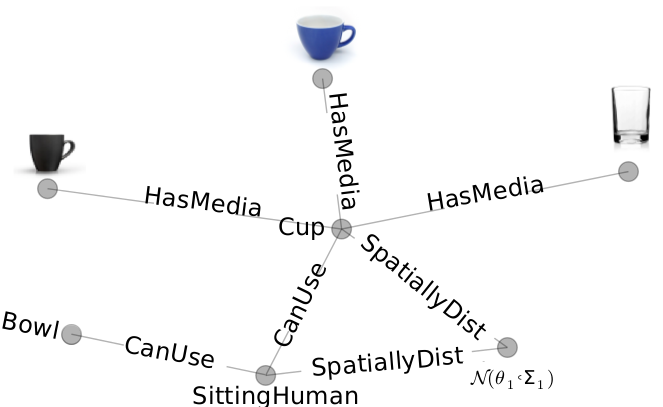
\includegraphics[width=0.48\textwidth]{before.png}}~\subfigure[feed insertion]{\label{a}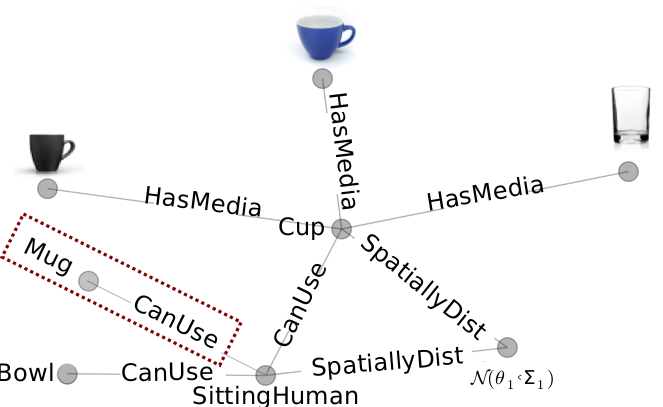
\includegraphics[width=0.48\textwidth]{insert.png}}

\subfigure[after $merge(Mug,Mug^\prime) \rightarrow Mug \circ split(Cup)\rightarrow(Cup,Mug^\prime)$]{\label{a}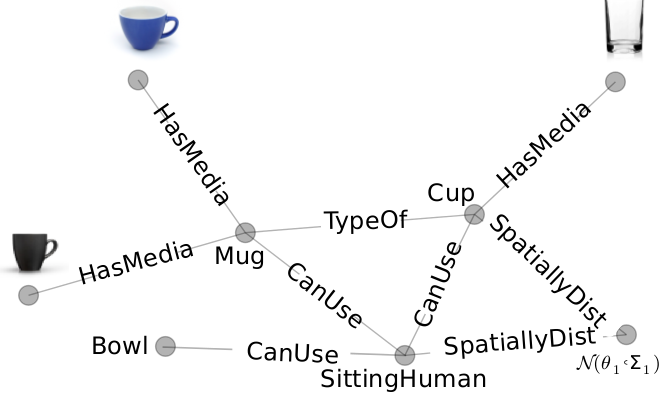
\includegraphics[width=0.48\textwidth]{after.png}}
\caption{\textbf{Visualization of inserting new information.} We insert `\emph{Sitting human can use a mug}' and \robobrain{} infers the necessary split and merge operations on the graph. In (a) we show the original sub-graph, In (b) information about a \emph{Mug} is seen for the first time and the corresponding node and edge are inserted, In (c) inference algorithm infers that previously connected cup node and  cup images are not valid any more, and it splits the $Cup$ node into two nodes as $Cup$ and $Mug^\prime$ and then merges $Mug^\prime$ and $Mug$ nodes.}
\label{insertgraph}
\end{figure}


\section{Knowledge Engine: Formal Definition}
\label{sec:graph}

In this section we present the formal definition of \mbox{\robobrain{}}.
\robobrain{} represents knowledge as a directed graph $\mathcal{G}=(V,E)$.
The vertices $V$ of the graph stores concepts that can  be of a variety
of types such as images, text, videos, haptic data, or  learned entities such as affordances, deep learning features, parameters, etc.
The edges $E \subseteq V\times V\times C$ are directed and represents the relations between concepts. Each edge has an edge-type from a set $C$ of possible edge-types.

An edge $(v_1,v_2,\ell)$ is an ordered set of two nodes $v_1$ and $v_2$ and an edge-type  $\ell$.
%connected by an edge type $\ell$ from $v_1$ to $v_2$.
% in which it represent there exist an edge from node $v_1$ to node $v_2$ with type $l$.
Few examples of such edges are: $($StandingHuman, Shoe, \emph{CanUse}$)$,
$($StandingHuman, $\mathcal{N}(\mu,\Sigma)$, \emph{SpatiallyDistributedAs}$)$
and $($Grasping, DeepFeature$23$, \emph{UsesFeature}$)$. %These edges can be considered as (\emph{subject}, \emph{object}, \emph{predicate}) triplets.
We do not impose any constraints on the type of data that nodes can represent. However, we require the edges to be consistent with \robobrain{} edge set $C$. We further associate each node and edge in the graph with \textit{a feature vector representation} and a \textit{belief}. The feature vector representation of nodes and edges depend on their local connections in the graph, and their belief is a scalar probability over the accuracy of the information that the node or an edge represents. Tables~\ref{tbl:vertices} and~\ref{tbl:edges} show few examples of nodes and edge-types. A snapshot of the graph is shown in  Figure~\ref{fig:graph}.

\subsection{Creating the Graph}
Graph creation consists of never ending cycle of two stages namely, knowledge acquisition and inference. Within the knowledge acquisition stage, we collect data from various sources and during the inference stage we apply statistical techniques to update the graph structure based on the aggregated data. We explain these two stages below.



\smallskip
\noindent{\textbf{Knowledge acquisition:}} \robobrain{} accepts new information in the form of set of edges, which we call a \textit{feed}. A \textit{feed} can either be from an automated algorithm crawling the Internet sources or from one of \robobrain{}'s partner projects.
We add a new \textit{feed} to the existing graph through a sequence of union operations performed on the  graph. These union operations are then followed by an inference algorithm.
More specifically, given a new \emph{feed} consisting of a set of $N$ edges \{$(v^1_1,v^1_2,\ell^1) \ldots (v^N_1,v^N_2,\ell^N)$\}, and the existing graph $G = (V,E)$. The graph union operations give a graph $G^\prime=(V^\prime,E^\prime)$ as follows:
\begin{equation}
\label{eq:update}
\begin{aligned}
V^\prime &= v^1_1 \cup v^1_2 \cup \ldots \cup v^N_1 \cup v^N_2 \cup V \\
E^\prime &=  (v^1_1,v^1_2,\ell^1) \cup \ldots \cup (v^N_1,v^N_2,\ell^N) \cup E
\end{aligned}
\end{equation}

%\noindent
%After the knowledge is acquired, we update the graph in the next step.

\smallskip
\noindent{\textbf{Inference on the Graph:}}
After adding the \textit{feed} to the graph using equation~\eqref{eq:update}, we perform inference to update the graph based on this new knowledge. The inference outputs a sequence of graph operations which are then performed on the graph. These graph operations modify the graph by adding new nodes or edges to the graph, deleting nodes or edges from the graph, merging or splitting nodes, etc.

We mention two graph operations here: \emph{split} and \emph{merge}. The split operation is defined as splitting a node into a set of two nodes. The edges having end points in the split node are connected to one of the resultant nodes using the inference algorithm. A merge operation is defined as merging two nodes into a single node, while updating the edges connected to the merged nodes. An example of such an update is shown in Figure \ref{insertgraph}. When a new information \emph{``sitting human can use a mug"} is added to the graph, it causes the \textit{split} of the \emph{Cup} node into two nodes: a \emph{Cup} and a \emph{Mug} node. These two are then connected by an edge-type \textit{TypeOf}. The graph update can be expressed through the following equation:
$$G^\star = split_{v_{s_1}} \circ merge_{v_{m_1},v_{m_2}} \circ \ldots \circ split_{v_{s_M}} \circ G^\prime$$

In the above equation $G^\star$ is the graph obtained after the inference. The goal of the inference steps is to modify the graph $G^\prime$ in a way that best explains the physical world. However, the graph that captures the real physical world is a  \textit{latent graph}, i.e., it is not directly observable.
For  example, the latent information that \emph{``coffee is typically in a container"} is partially observed through
many edges between the \emph{coffee} node and the nodes with \emph{container} images. Our graph construction can also be explained in a generative setting of having a latent graph with all the knowledge about physical word, and we only observe  noisy measurements in form of \textit{feeds}. In this paper, we abstract the algorithmic details of inference and focus on the overall ideas involved in \robobrain{}, its architecture, and its application to robotics.
%system architecture and presenting the overall ideas in the RKE, and defer the details of inference algorithms and the latent graph to a later journal version.



\begin{table}
\caption{Some examples of different node types in our \robobrain{} graph. For full-list,
please see the code documentation.}
\label{tbl:vertices}
\begin{tabular}{ll}
Word & an English word represented as an ASCII string\\
DeepFeature & feature function trained with a Deep Neural Network\\
Image & 2D RGB Image\\
PointCloud & 3D point cloud\\
Heatmap & heatmap parameter vector\\
\end{tabular}
\end{table}
\begin{table}
\caption{Some examples of different edge types in our \robobrain{} graph. For full-list,
please see the code documentation.}
\label{tbl:edges}
\begin{tabular}{ll}
IsTypeOf & human \emph{IsTypeOf} a mammal \\
HasAppearance & floor \emph{HasAppearance} as follows (this image) \\
CanPerformAction & human \emph{CanPerformAction} cutting \\
SpatiallyDistributedAs & location of human is \emph{SpatiallyDistributedAs} \\
IsHolonym & tree  \emph{IsHolonym} of leaf
\end{tabular}
\vskip -.2in
\end{table}




% !TEX root = robobrain.tex
\section{System Architecture}
\label{sec:system}
\begin{figure}[t]
\centering
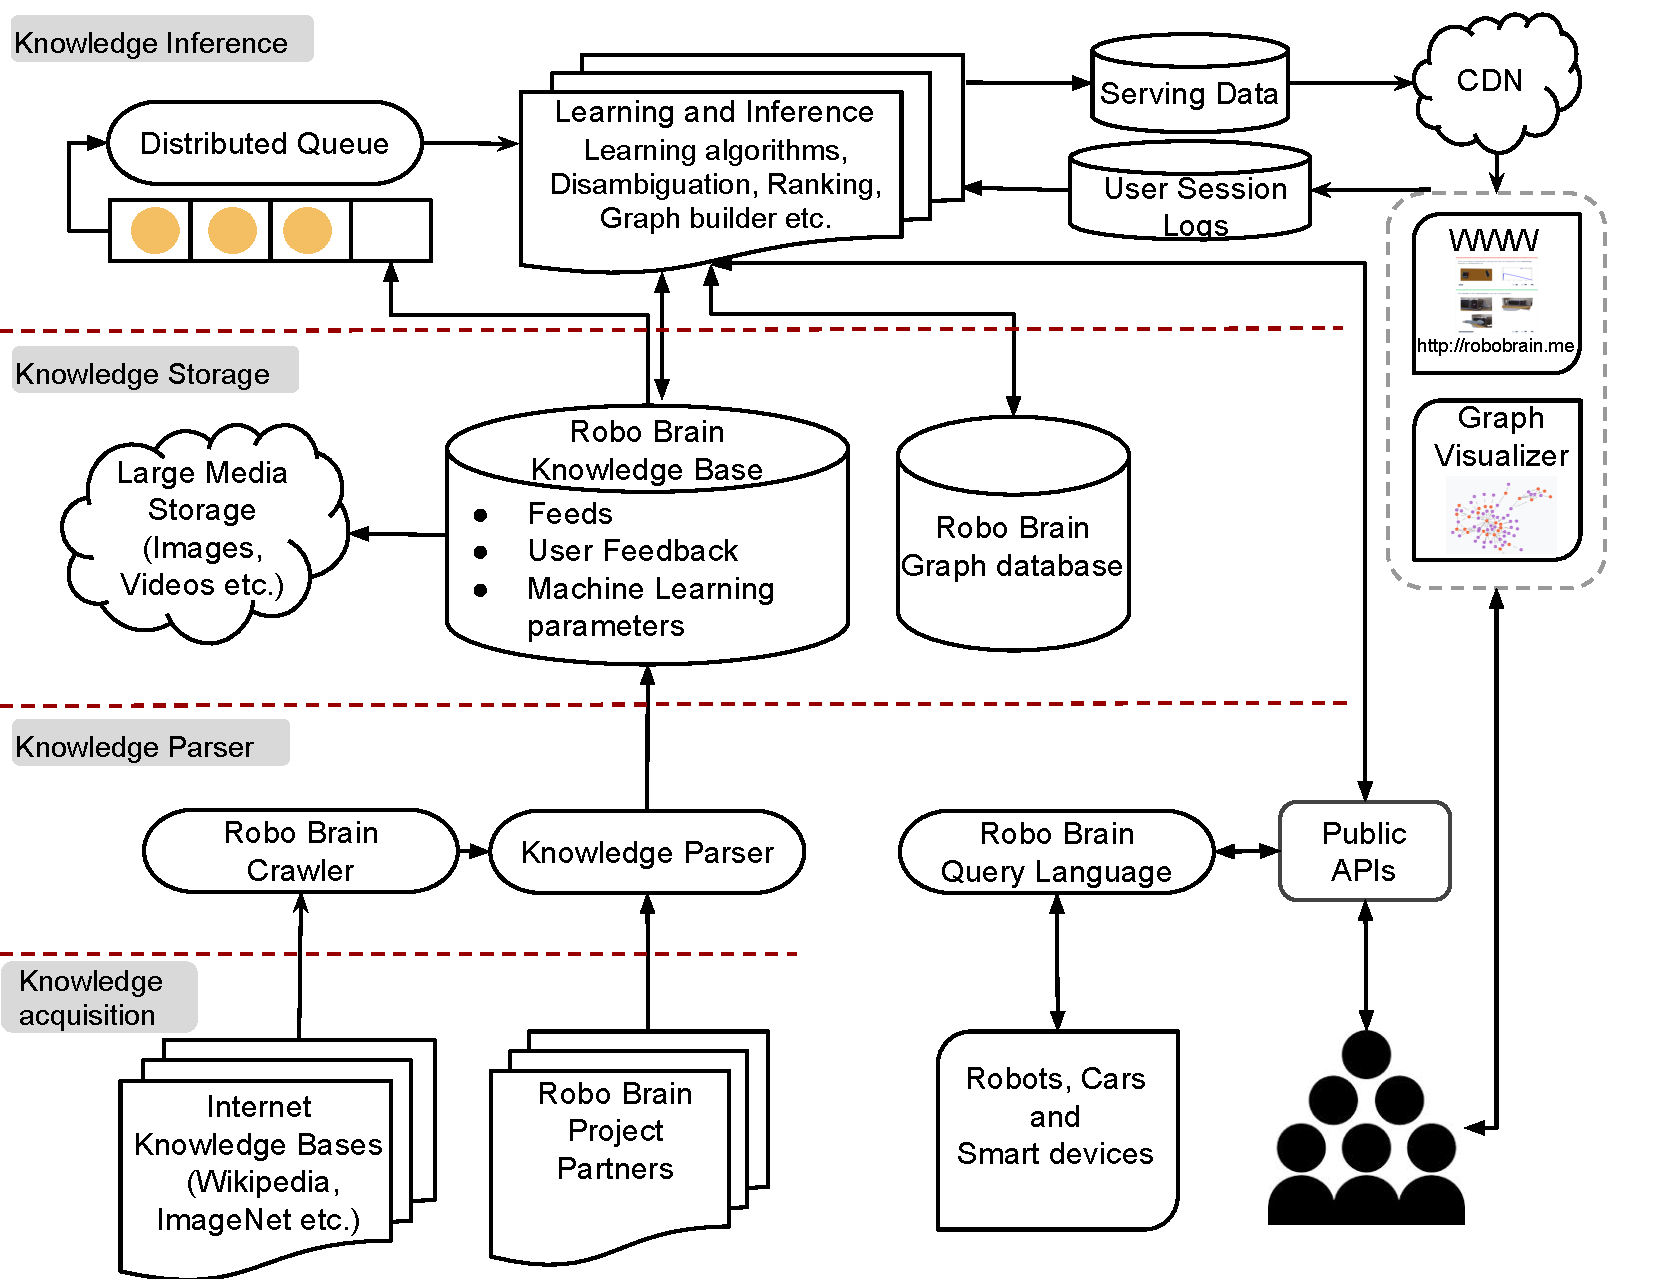
\includegraphics[width=\linewidth]{Image/RoboBrain_Systems}
%\vskip -.1in
\caption{\textbf{\robobrain{} system architecture.} It consists of four
interconnected knowledge layers and supports various mechanisms for users and
robots to interact with \robobrain{}.}
\label{fig:system}
\end{figure}

% \todo {This is just a first pass to set the basic coverage of the section}

We now describe the system architecture of \robobrain{}, shown in Figure~\ref{fig:system}. The system
consists of four interconnected layers: (a) knowledge acquisition, (b) knowledge
parser, (c) knowledge storage,  and (d) knowledge inference. The principle
behind our design is to efficiently process large amount of unstructured
multi-modal knowledge and represent it using the structured \mbox{\robobrain{}} graph.
In addition, our design also supports various mechanisms for users and robots to interact with \robobrain{}. %Through these interactions users retrieve knowledge and also improve \robobrain{} through feedback. 
Below we discuss each of the components.
%and (e) interaction mechanisms.

% It also comprises interactions with robots and users via physical and online interactions.

% many layers and most of the components are restful (Need to write more).

\textit{Knowledge acquisition} layer is the interface between \robobrain{} and the
different sources of multi-modal data. Through this layer \robobrain{} gets access to new information which the other layers process.  \robobrain{} primarily collects knowledge through its partner projects and by crawling the existing knowledge bases such as Freebase, ImageNet and WordNet, etc.,  as well as unstructured sources such as  Wikipedia.


\textit{Knowledge parser} layer of \robobrain{} processes the data acquired by the acquisition layer and converts it to a consistent format for the storage layer. It also marks the incoming data with appropriate meta- data such as  timestamps, source version number etc., for scheduling and managing future data processing. Moreover, since the knowledge bases might change with time, it adds a back pointer to the original source.

\textit{Knowledge storage} layer of \robobrain{} is responsible for storing different representations of the data. In particular it consists of a NoSQL document storage database cluster -- \robobrain{} Knowledge Base (\robobrain{}-KB) -- to store ``feeds'' parsed by the knowledge parser, crowd-sourcing feedback from users, and parameters of different machine learning algorithms provided by \robobrain{} project partners. \robobrain{}-KB offloads large media content such as images, videos and 3D point clouds to a distributed object storage system built using Amazon Simple Storage Service (S3). The real power of \robobrain{} comes through its graph database (\robobrain{}-GD) which stores the structured knowledge. The data from \robobrain{}-KB is refined through multiple learning algorithms and its graph representation is stored in \robobrain{}-GD. The purpose behind this design is to keep \robobrain{}-KB as the \robobrain{}'s single source of truth (SSOT). SSOT centric design allows us to re-build \robobrain{}-GD in case of failures or malicious knowledge sources.

\textit{Knowledge inference} layer contains the key processing and machine learning components of \robobrain{}. All the new and recently updated feeds go through a persistent replicated distributed queuing system (Amazon SQS), which are then consumed by some of our machine learning plugins (inference algorithm, graph builder, etc.) and populates the graph database. These plugins along with  other learning algorithms (operating on the entire graph) constitute our learning and inference framework. 

\robobrain{} supports various \textit{interaction mechanisms} to enable robots and users to communicate with the knowledge engine.
We develop a Robot Query Library as a primary method for robots to interact with \robobrain{}. We also make available a set of public APIs to allow information to be presented on the WWW for online learning mechanisms (eg., crowd-sourcing). \robobrain{} serves all its data using a commercial content delivery network (CDN) to reduce the end user latency. 

% !TEX root = robobrain.tex
\section{Robot Query Library (RQL)}
\label{sec:raquel}
In this section we present the RQL query language,
through which the robots use \robobrain{} for various robotic applications.
The RQL provides a rich set of \textit{retrieval functions} and \textit{programming constructs} to
perform complex traversals on the \robobrain{} graph. An example of such a query is finding the possible ways
for humans to use a cup. This query requires traversing paths from the human node to the cup node in
the \robobrain{} graph.

The RQL allows expressing both the \textit{pattern} of sub-graphs to match and the
\textit{operations} to perform on the retrieved information. An example of such an operation is
\textit{ranking} the paths from the human to the cup node in the order of relevance. The RQL admits following two types of functions: (i) graph retrieval
functions; and (ii) programming construct functions.

\subsection{Graph retrieval function}
The graph retrieval function is used to find sub-graphs matching a given \textit{template} of the form: $$\text{Template: }(u)\rightarrow [e] \rightarrow (v)$$
In the template above, the variables $u$ and $v$ are nodes in the graph and the variable $e$ is a directed edge from $u$ to $v$. We represent the graph retrieval function with the keyword ${\tt fetch}$ and the corresponding RQL query takes the following form:
$${\tt fetch}(\text{Template})$$
The above RQL query finds the sub-graphs matching the template. It instantiates the variables in the template to match the sub-graph and returns the list of instantiated variables. We now give a few use cases of the retrieval function for \robobrain{}.

\begin{example}
The RQL query to retrieve all the objects that a human can use
\begin{align*}
\text{Template: }&{\tt(\{name:`Human'\})\rightarrow [`CanUse'] \rightarrow (v)}\\
\text{Query: }&{\tt fetch}(\text{Template})
\end{align*}
The above query returns a list of nodes that are connected to the node with name ${\tt{Human}}$ and with an edge of type ${\tt{CanUse}}$.% We  now give a query example for retrieving nodes that not directly connected.
\end{example}
Using the RQL  we can also express several \textit{operations} to perform on the retrieved results.
The operations can be of type   ${\tt SortBy}$, ${\tt Len}$, ${\tt Belief}$ and ${\tt ArgMax}$. We now
explain some of these operations with an example.
\begin{example}
The RQL query to retrieve and sort all possible paths from the ${\tt{Human}}$ node to the ${\tt{Cup}}$ node.
%\noindent \resizebox{\linewidth}{!}{
%\begin{minipage}{\linewidth}
\vskip -0.13in
{\small
\begin{align*}
 &{\tt paths }:= \;{\tt fetch (\{name:`Human'\})\rightarrow [r *] \rightarrow (\{name:`Cup'\})}\\
& {\tt SortBy(\lambda P \rightarrow Belief \, P) \, paths} \\
\end{align*}
%\end{minipage}
}\vskip -0.15in

In the example above, we first define a function ${\tt paths}$ which returns all  the paths from the node ${\tt Human }$ to the node ${\tt Cup }$ in the form of a list. The ${\tt SortBy}$ query first runs the ${\tt paths}$ function and then sorts, in decreasing order, all paths in the returned list using their beliefs.
\end{example}


\subsection{Programming construct functions}
The programming construct functions serve to process the sub-graphs retrieved by the graph retrieval function ${\tt fetch}$. In order to define these functions we make use of functional programming constructs like ${\tt map}$, ${\tt filter}$ and ${\tt find}$. We now explain the use of some of these constructs in RQL.

\begin{example}
The RQL query to retrieve affordances of all the objects that ${\tt{Human}}$ can use.
\vskip -0.13in
%\noindent \resizebox{\linewidth}{!}{
%\begin{minipage}{\linewidth}
{\small
\begin{align*}
&  {\tt objects }:=\; {\tt fetch (\{name:`Human'\})\rightarrow [`CanUse'] \rightarrow (v)} \\
&  {\tt affordances \;n } := \;{\tt fetch (\{name:n\})\rightarrow [`Has Affordance'] \rightarrow (v)} \\
&  {\tt map(\lambda u \rightarrow affordances \, u) \,  objects} \\
\end{align*}
%\end{minipage}
}\vskip -0.15in

\noindent In this example, we illustrate the use of ${\tt map}$ construct. The ${\tt map}$ takes as input a function and a list, and then applies the function to every element of the list. More specifically, in the example above, the function ${\tt objects }$ retrieves the list of objects that the human can use. The ${\tt affordances }$ function takes as input an object and returns its affordances. In the last RQL query, the ${\tt map}$  applies the function ${\tt affordances}$ to the list returned by the function ${\tt objects}$.
\end{example}
We now conclude this section with an expressive RQL query for retrieving \textit{joint parameters} shared among nodes. Parameters are one of the many concepts we store in \robobrain{} and they represent learned knowledge about nodes. The algorithms use joint parameters to relate multiple concepts and here we show how to retrieve joint parameters shared by multiple nodes. In the example below, we describe the queries for parameter of a single node and parameter shared by two nodes.

\begin{example}
\label{ex:joint}
The RQL query to retrieve the joint parameters shared between a set of nodes.
\vskip -0.13in
%\noindent \resizebox{\linewidth}{!}{
%\begin{minipage}{\linewidth}
{\small
\begin{align}
&{\tt {parents} \,\, n := fetch \,\, (v)\rightarrow [`HasParameters']\rightarrow  (\{handle:n\}) }\nonumber \\
& {\tt {parameters} \,\, n :=  fetch \,\, (\{name:n\})\rightarrow [`HasParameters']\rightarrow }  (v)  \nonumber  \\
& {\tt {ind\_parameters}\;\; a := }  \cr
&{\tt \hspace*{2cm} filter (\lambda u \rightarrow\! {Len \; parents}\; u = 1)     {parameters}\, a \nonumber } \\
& {\tt {joint\_parameters} \,\, a_1 \,\, a_2\,\, := } \cr
& {\tt \hspace*{2cm} filter (\lambda u \rightarrow {Len\; parents}\,\, u = 2\,\, and } \cr
& {\tt \hspace*{2cm}  u \,\, in \,\, {parameters}\,\, a_2)    \,\,{parameters}\,\, a_1 \nonumber}
\end{align}
%\end{minipage}
}\vskip -0.01in
The query above uses the ${\tt filter}$ construct function and ${\tt Len}$ operation. The ${\tt filter}$ takes as input a list and a check condition, and returns only those items from the list that satisfies the input condition. The ${\tt Len}$ takes as input a list and returns the number of items in the list.
In the query above, we first define a function ${\tt parents}$ which for a given input node returns its parent nodes. Then we define a function ${\tt parameters}$ which for a given input node returns its parameters. The third and the fourth queries are functions accepting one and two input nodes, respectively, and return the (joint) parameters that share an edge with every input node and not with any other node.
\end{example}

% !TEX root = ../../ozan_sener_thesis.tex
\section{Applications}
\label{sec:applications}
In this section we first show how \robobrain{} can be used \textit{as-a-service} by the robots for several robotics problems. Specifically, we explain the usage of \robobrain{} in anticipating human activities, grounding of natural language sentences, and path planning. We then show how \robobrain{} can help robotics projects by sharing knowledge within the projects and throughout the Internet.

\subsection{\robobrain{} \textit{as-a-service}}
Our goal with providing \robobrain{} \textit{as-a-service} is to allow robots to use the representations learned by different partner projects. 
% For this purpose the 
% RKE stores the representations learned by different projects, allows queries through RQL. 
This 
% feature of the RKE 
allows \robobrain{} to effortlessly address many robotics applications. In the following we demonstrate \robobrain{} as-a-service feature for three robotics applications that deal with different data modalities of perception, natural language and trajectories.

% !TEX root = ../../ozan_sener_thesis.tex
\begin{figure}
\centering
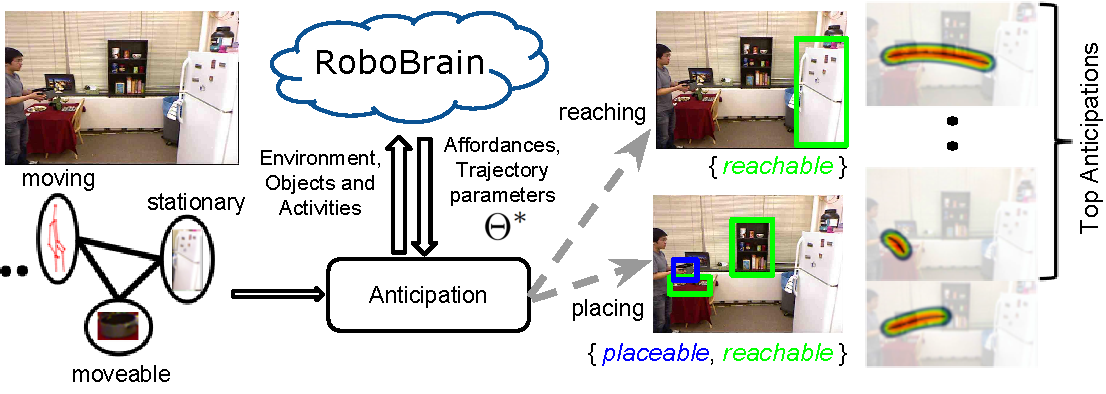
\includegraphics[width=\linewidth]{./Image/anticipation_robobrain_pic.pdf}
\caption{\textbf{\robobrain{} for anticipating human activities.} Robot using anticipation algorithm of \citet{KoppulaRSS2013} queries \robobrain{}, for the activity, affordance and trajectory parameters in order to generate and rank the possible future activities in a given environment.}
\label{Fig:anticipation}
\end{figure}

\subsubsection{Anticipating human actions}
\label{sec:anticipation}
The assistive robots working with humans should be able to understand human activities and also anticipate the future actions that the human can perform. In order to anticipate, the robot should reason over the action possibilities in the environment, i.e., \textit{object affordances}, and how the actions can be performed, i.e., \textit{trajectories}. Several works in robotics have addressed the problem of anticipation~\citep{KitaniECCV2012,KoppulaRSS2013,Kuderer-RSS-12}.

We now show how robots can query \robobrain{} and use the previous work by
Koppula et al.~\citep{KoppulaRSS2013} for anticipating human actions.  
In order to anticipate the future human actions, the authors~\citep{KoppulaRSS2013} learn parameters using their anticipatory algorithm, and using the learned parameters they anticipate the most likely \textit{future} object affordances and human trajectories. \robobrain{} serves anticipation \textit{as-a-service} by storing those learned parameters, object affordances and trajectories  as concepts in its graph. Figure~\ref{Fig:anticipation} illustrates a robot retrieving relevant information for anticipation. The robot first uses the following queries to retrieve the possible trajectories of an object:

%\noindent \resizebox{\linewidth}{!}{
%\begin{minipage}{\linewidth}
{\small
\begin{align}
&{\tt {affordances} \,\, n := fetch \,\,(\{name:n\})\rightarrow   [`HasAffordance'] \rightarrow } \cr
& {\tt \hspace*{2cm} (v\{src:`Affordance'\})   \nonumber } \\
&{\tt {trajectories} \,\, a := fetch \,\,(\{handle:a\})\rightarrow [`HasParameters']\rightarrow } \cr
& {\tt \hspace*{2cm}  (v\{src:`Affordance', type:`Trajectory'\})  \nonumber } \\
& {\tt { trajectory\_parameters} \,\, o := \,\, } \cr
&{\tt \hspace*{2cm} map (\lambda a \rightarrow {trajectories}\,\, a)  \,\, {affordances}\,\, o } \nonumber
\end{align}
%  \end{minipage}
}


In the queries above, the robot first queries for the affordances of the object and then for each affordance it queries \robobrain{} for the trajectory parameters. Having retrieved all possible trajectories, the robot uses the learned parameters~\citep{KoppulaRSS2013} to anticipate the future human actions. Since the learned parameters are also stored in the \robobrain{} graph, the robot retrieves them using the following RQL queries:
{\small
\begin{align*}
&{\tt {parents} \,\, n := fetch \,\, (v)\rightarrow [`HasParameters']\rightarrow  (\{handle:n\}) }\nonumber \\
& {\tt {parameters} \,\, n :=  fetch \,\, (\{name:n\})\rightarrow [`HasParameters']\rightarrow }\cr
& {\tt \hspace*{2cm}  (v\{src:`Activity'\})   \nonumber } \\
& {\tt find\_parameters\, a := }\\
& \hspace*{2cm}{\tt filter (\lambda u \rightarrow\! {Len\; parents}\, u = 1)     {parameters}\, a \nonumber } \\
& {\tt {joint\_parameters} \,\, a_1 \,\, a_2\,\, := filter (\lambda u \rightarrow {Len\; parents}\,\, u = 2\,\, } \cr
& {\tt \hspace*{2cm}  and\,\, u \,\, in \,\, {parameters}\,\, a_2)    \,\,{parameters}\,\, a_1 \nonumber}
\end{align*}
}
The queries above retrieves both independent and joint parameters for anticipating the object affordances and human activities. Detailed explanation of the query is given in Example \ref{ex:joint} of Section \ref{sec:raquel}



% !TEX root = robobrain.tex

\subsubsection{Grounding natural language} The problem of grounding a natural language instruction in an environment requires the robot to formulate an action sequence  that accomplish the semantics of the  instruction~\citep{tellex2011understanding,misra2014tell,guadarrama2013grounding, MatuszekISER2012}. In order to do this, the robot needs a variety of information. Starting with finding action verbs and objects in the instruction, the robot has  to discover those objects and their affordances in the environment.

% \robobrain{} provides natural language grounding \textit{as-a-service}.

We now show the previous work by Misra et al.~\cite{misra2014tell} using \robobrain{} \textit{as-a-service} in their algorithm. In order to ground a natural language instruction the robot has to check for the satisfiability of the actions it generates in the given environment. For example, an action which pours water on a book should be deemed unsatisfiable. In the previous work~\cite{misra2014tell}, the authors manually define many pre-conditions to check the satisfiability of actions. For example, they define manually that a \textit{syrup bottle} is \textit{squeezable}. Such satisfiability  depends on the object's affordances in the given environment, which can be retrieved from \robobrain{}.

Figure~\ref{Fig:languagegrounding} illustrates a robot querying \robobrain{} to check the satisfiability of actions that it can perform in the given environment. Below is the RQL query for retrieving the satisfiability of  \textit{squeezable} action:
%\noindent \resizebox{\linewidth}{!}{
%\begin{minipage}{\linewidth}
{\small
\begin{align*}
&{\tt {squeezable \,\ syrup}\,\,  := \,\,Len \,\,fetch \,\,(u\{name:`syrup'\})\rightarrow }\\
&{\tt \hspace*{0.1cm} [`HasAffordance']\rightarrow (v\{name:`squeezable'\})\,\,> 0}
\end{align*}
%  \end{minipage}
}

\begin{figure}[t]
\centering
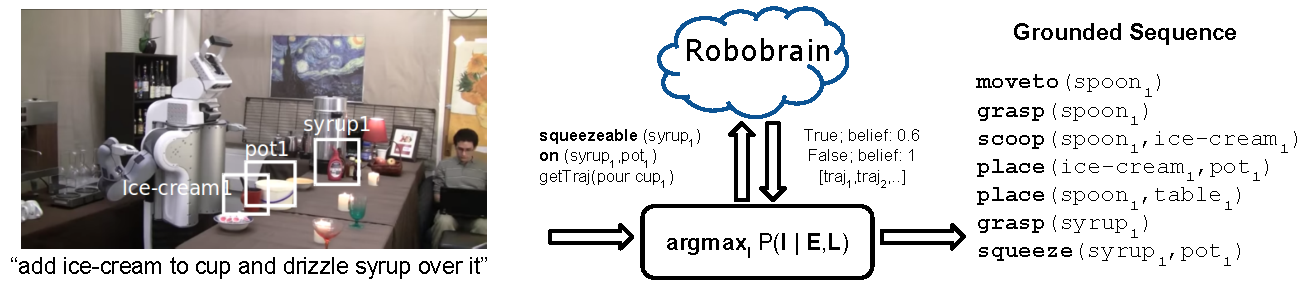
\includegraphics[width=1\linewidth]{./Image/tellmedave_robobrain_pic.pdf}
\caption{\textbf{Grounding natural language sentence.} The robot grounds natural language by using the algorithm by Misra et al.~\cite{misra2014tell} and querying \robobrain{} to check for the satisfiability of actions.}
%\cite{misra2014tell} requires several  pieces of knowledge. Robot should know the appearances and affordances of objects, as well as the possible actions related to each object and it should know the trajectories and manipulation features of those actions. These are all  translated as queries to the RKE graph.}
\label{Fig:languagegrounding}
\end{figure}
%% !TEX root = robobrain.tex
\subsubsection{Path planning using \robobrain{}}
\label{sec:applicationplanit}

One key problem robots face in performing tasks in human environments is identifying trajectories desirable to the users. An appropriate trajectory not only needs to be valid from a geometric standpoint (i.e., feasible and obstacle-free), but it also needs to satisfy the user preferences~\citep{jainsaxena2013_trajectorypreferences,Jain14}. For example,  a robot should move sharp objects such as knife strictly away from nearby humans~\cite{jain_contextdrivenpathplanning_2013}. Such preferences are commonly represented as cost functions which jointly model the environment, the task, and trajectories.
%This joint modeling is expensive in terms of resource requirement (e.g., robots) and data collection, and
Typically research groups have independently learned different cost functions~\citep{jainsaxena2013_trajectorypreferences,Kuderer-RSS-12,KitaniECCV2012}, which are not shared across the research groups. Here we show \robobrain{} \textit{as-a-service}  for a robot to store and retrieve the planning parameters.
%We now show how the previous work by Jain et al.~\citep{Jain14} use the RKE for retrieving the trajectory parameters for path planning. We demonstrate this on the example of moving an egg carton from the previous work~\citep{Jain14}.

In Figure~\ref{fig:planning} we illustrate the robot planning for an egg carton by querying \robobrain{}.
Since eggs are \textit{fragile}, users  prefer to move them slowly and close to the surface of the table.  In order to complete the task, the robot queries \robobrain{} and retrieves the attributes of the egg carton and also the trajectory parameters learned in the previous work by Jain et al.~\citep{Jain14}. Using the retrieved attributes and the parameters, the robot samples trajectories and executes the top-ranked trajectory.
%need labels of all objects in the environment. In this example we use the
%object labels provided by the authors~\cite{Jain14}. After the object labels are obtained, the previous
%work~\citep{Jain14} use the RKE to retrieve attributes of the egg carton and also the trajectory
%parameters.
Below we show the RQL queries.
%\noindent \resizebox{\linewidth}{!}{
%\begin{minipage}{\linewidth}
{\small
\begin{align*}
&{\tt {attributes} \,\, n := fetch \,\,(\{name:n\})\rightarrow
[`HasAttribute'] \rightarrow (v)   \nonumber} \\
&{\tt {trajectories} \,\, a := }\\
&{\tt\hspace*{2cm} fetch \,(\{handle :a\})\rightarrow  [`HasTrajectory'] \rightarrow (v)  \nonumber } \\
&{\tt {trajectory\_parameters} := }\\
&{\tt \hspace*{2cm} map (\lambda a \rightarrow
{trajectories}\,\, a)  \,\, {attributes}\,\, `egg' } \nonumber
\end{align*}
%  \end{minipage}
}

\begin{figure}[t]
\centering
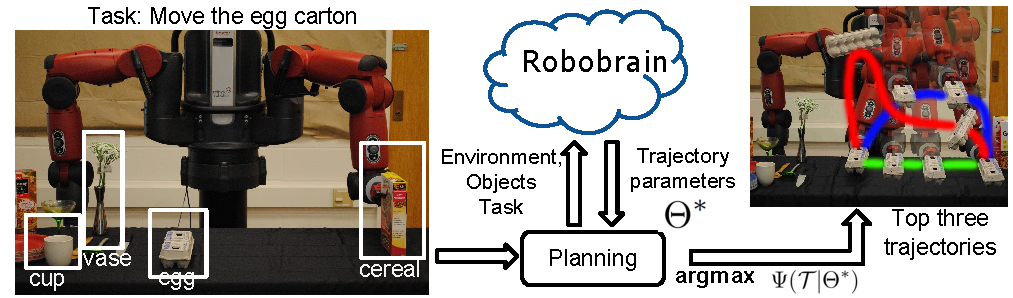
\includegraphics[width=\linewidth]{Image/planit_robobrain_pic_2}
\caption{\textbf{\robobrain{} for planning trajectory.} The robot queries \robobrain{} for the trajectory parameters (learned by Jain et al.~\citep{jainsaxena2013_trajectorypreferences})  to plan paths for the fragile objects like an egg carton. }
\label{fig:planning}
\end{figure}

% !TEX root = ../../ozan_sener_thesis.tex


\subsection{\robobrain{} for sharing knowledge}
\robobrain{} allows sharing the knowledge learned by different research groups as well as knowledge obtained from various internet sources. In this section we show with experiments how sharing knowledge improves existing robotic applications:

\iffalse
\subsubsection{Sharing knowledge from the Internet}
In this experiment we show that sharing knowledge from several Internet sources using \robobrain{} improves robotic applications such as path planning.  Knowledge from the Internet sources has been shown to help robots in planing better paths~\citep{beetzIcra2010}, understand natural language~\citep{coyneCosli,tellex2011understanding}, and also recently in object retrieval~\citep{guadarramaRss2014}. However, for certain robotic tasks a single Internet source does not cover many of the real world situations that the robot may encounter. In such situations it is desired to share the information from other sources to get an overall richer representation.
The \robobrain{} graph is designed to acquire and connect information from multiple Internet sources and make it accessible to robots.

In this experiment we build upon work by Jain et al.~\citep{jainsaxena2013_trajectorypreferences} for planning trajectories that follow user preferences. The work relied on object attributes in order to plan desirable trajectories. These attributes convey properties such as whether an object is sharp, heavy, electronic etc. The attributes were manually defined by the authors~\citep{jainsaxena2013_trajectorypreferences}. In practice this is very challenging and time-consuming because there are many objects and many attributes for each object.
%Jain et al.~\citep{jainsaxena2013_trajectorypreferences}  manually define attributes used by TPP.
Instead of manually defining the attributes, we can retrieve many of them from the Internet knowledge
sources such as OpenCyc, Wikipedia, etc. However, a single knowledge source might not have
attributes for all objects.
The \robobrain{} graph connects many attributes obtained from multiple Internet sources to their respective objects.
%We crawl multiple internet sources to retrieve many attributes and connect them to their respective objects in the \robobrain{} graph.


\begin{figure}
\centering
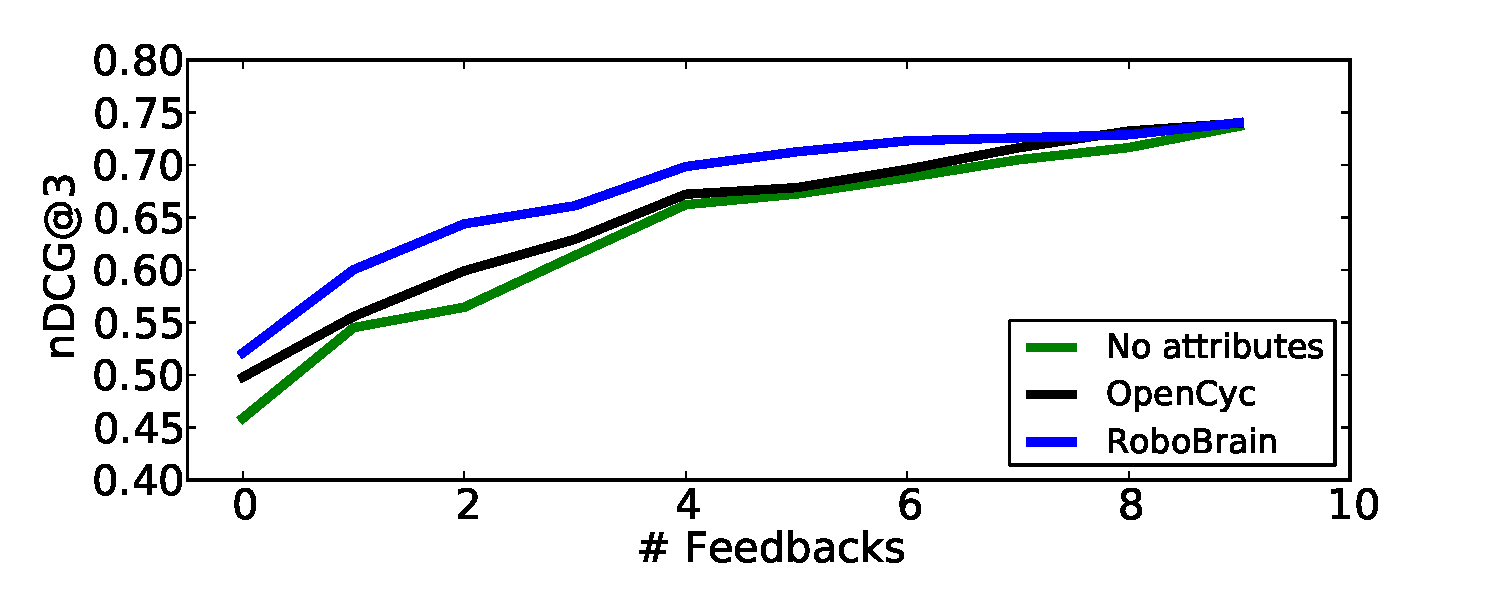
\includegraphics[width=\linewidth]{Image/internet_attributes}
\caption{\textbf{Sharing from Internet sources.} The plot shows performance of  the algorithm by Jain et al.~\citep{jainsaxena2013_trajectorypreferences} for three settings of attributes. This is an online algorithm that learns a good trajectory from the user feedback. The performance is measured using the nDCG metric~\cite{manning2008introduction}, which represents the quality of the ranked list of trajectories. \robobrain{} combines information from multiple sources and hence its richer in attributes as compared to retrieving attributes from OpenCyc alone.}
\label{fig:ndcg}
\end{figure}

Figure~\ref{fig:ndcg} illustrates the planning results when the robot does not use any attributes, when it uses attributes from a single source (OpenCyc), and when it use attributes from \robobrain{}. The planning performance is best when using \robobrain{} since it covers more attributes than the OpenCyc alone. Most importantly all these attributes are retrieved from the \robobrain{} graph with a single RQL query as explained in Section \ref{sec:applicationplanit}.
\fi

%\subsubsection{Sharing learned representations}

New algorithms are commonly proposed for a problem to address the shortcomings of previous methods. These algorithms have their own learned representations. For example,  different representations  have been learned for grounding natural language~\citep{tellex2011understanding,misra2014tell,guadarrama2013grounding, MatuszekISER2012}. However, it is usually hard for practitioners to choose a single representation since there are always inputs where one representation fails but some others work. In this experiment we show that a robot can query \robobrain{} for the best representation while being agnostic to the algorithmic details of the learned representations.

Simulating the above setting, we present an experiment for sharing multiple learned representations on a natural language grounding problem. Here the goal is  to output a sequence of instructions for the robot to follow, given an input natural language command and an environment.
Following the work by Misra et al.~\citep{misra2014tell}, we train a baseline algorithm for the task of \textit{making ramen} (Algorithm A), and train their full algorithm for the task of \textit{making affogato} (Algorithm B). These algorithms assign a  confidence score (i.e., probability) to the output sequence of instructions.  We store these learned representations as concepts in the \robobrain{} graph, along with a prior belief over the correctness of the algorithms. The robot queries \robobrain{} for a representation as follows:
%\resizebox{\linewidth}{!}{
%\begin{minipage}{\linewidth}
{\small
\begin{align*}
& {\tt algParam  :=  fetch (u\{type:'GroundingAlgorithm'\})}\rightarrow \\
& {\tt \hspace*{2cm} [`HasParameters'] \rightarrow (v)}   \\
& {\tt prior \,\, n :=  fetch (\{name:n\})\rightarrow [`HasPriorProb'] \rightarrow (v)}\\
& {\tt groundings \,\, L,E :=   argMaxBy(\lambda(u,v)\rightarrow v)} \\
& {\tt \hspace*{2cm} map(\lambda(u,v) \rightarrow u(L,E,v)*prior\, u) \, \, \, algParam}
\end{align*}
%\end{minipage}
}

\medskip
In the ${\tt algParam}$ function, we retrieve all natural language grounding algorithms from the \robobrain{} graph with their parameters. This returns a list in which each element is a tuple of algorithm $u$ and its parameters $v$. The ${\tt prior}$ function retrieves the prior belief over the correctness of an algorithm. In order to ground a given natural language command ${\tt L}$ in environment ${\tt E}$, the ${\tt grounding}$ function evaluates the likelihood score for each algorithm  using their parameters as ${\tt u(L,E,v)}$. It further incorporates the prior belief over the algorithms, and returns the representation with the highest likelihood score. These set of queries corresponds to the following likelihood maximization equation:
\begin{equation*}
\mathcal{I}^*  = \argmax_{\mathcal{I},m'\in \{A,B\}} P(\mathcal{I}|E, L,  w_{m'}^* ,m')P(m')
\end{equation*}
As shown in the Table~\ref{tbl:grounding-results}, choosing a representation by querying the \robobrain{} achieves better performance than the individual algorithms.

\begin{table}
\caption{\robobrain{} allows sharing learned representations. It allows the robot to query \robobrain{} for a representation given an input natural language command. In this table the Algorithm $A$ is a greedy algorithm based on Misra et al.~\cite{misra2014tell}, and Algorithm $B$ is their full model. The $IED$ metric measures the string-edit distance and the $EED$ metric measures the semantic distance between the ground-truth and the inferred output instruction sequences. The metrics are normalized to 100 such that higher numbers are better.}
\label{tbl:grounding-results}
\centering
\begin{tabular}{l|cc}
\hline
\textbf{Algorithm} & \textbf{IED} & \textbf{EED}\\
\hline
Algorithm A & 31.7 & 16.3\\
Algorithm B & 23.7 & \textbf{27.0}\\
\robobrain{} (A+B) & \textbf{34.2} & 24.2\\
\hline
\end{tabular}
\end{table}




% !TEX root = ../../ozan_sener_thesis.tex
\section{Discussion and Conclusion}
The \robobrain{} graph currently has 44347 nodes (concepts) and 98465 edges (relations). The knowledge in the graph is obtained from the Internet sources and through the \robobrain{} project partners. For the success of many robotics application it is important to relate and connect the concepts from these different knowledge sources. In order to empirically evaluate the connectivity of  concepts in \robobrain{}, we plot the degree distribution of the \robobrain{} graph and compare it with the degree distribution of independent knowledge sources (Figure~\ref{degDis}).
The graph of independent knowledge sources is the union of each knowledge source, which have nodes from all the projects and the edges only between the nodes from the same project.
As shown in the Figure~\ref{degDis}, \robobrain{} successfully connects projects and increases the average degree per-node by $0.8$.
\begin{figure}[h!]
 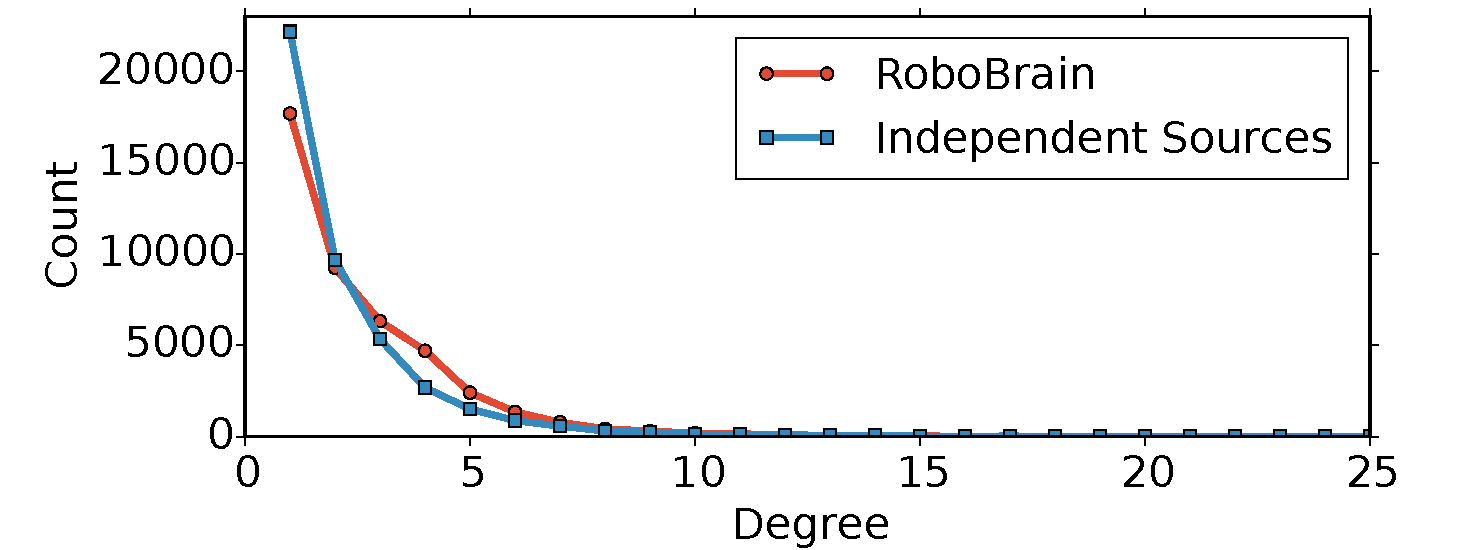
\includegraphics[width=\linewidth, height=1.5in]{Image/deg}
 \caption{Degree distribution of \robobrain{} and the union of independent knowledge sources.
 For the case of independent sources, we only consider the edges between nodes from the same
 source. \robobrain{} connects different projects successfully: number of nodes with degree 1 and 2 decrease and  nodes with degree 3 and more increase.}
\label{degDis}
\end{figure}
The \robobrain{} graph has fifteen thousand nodes with degree one. Most of the nodes with a single degree come from the Internet sources such as Wikipedia  and WordNet. These nodes are not directly related to the physical world and represent abstract concepts like political ideas, categories of art, etc.

In this chapter we described different aspects and technical challenges in building \robobrain{} knowledge engine. \robobrain{} represents multiple data modalities from various sources, and connects them to get an overall rich graph representation.  We presented an overview of the \robobrain{} large-scale system architecture and developed the Robot Query Library (RQL) for robots to use \robobrain{}. We illustrated robotics applications of anticipation, natural language grounding, and path planning as simple RQL queries to \robobrain{}. We also showed in experiments that sharing knowledge through \robobrain{} improves existing path planning and natural language grounding algorithms.
 \robobrain{} is an ongoing effort where we are collaborating with different research groups. We are working on improving different aspects such as learning from crowd-sourcing feedback, inference methods over the graph for discovering new relations between concepts, and expanding \robobrain{} to new robotics applications.

\iffalse
\robobrain{} is an ongoing effort, where we are constantly improving different aspects of the work.
% We are improving the system architecture and expanding RQL to support scaling to even larger
% knowledge sources (e.g., millions of videos).
% Furthermore,  w
We have several ongoing research efforts that include achieving
better disambiguation and improving never-ending learning abilities.
More importantly, we are constantly expanding the set of our \robobrain{} research partners.
This will not only improve the abilities of their robots, but also their contribution of knowledge
to \robobrain{} will help other researchers in the robotics community at large.
\fi


\chapter{Perception at Scale - Recursive Conditional Random Fields}
\epigraph{---~ Alice: How long is forever? \\ ---~ White Rabbit: Sometimes, just one second.}{\textit{Lewis Carroll\\ Alice's Adventures in Wonderland}}

% !TEX root = ../../ozan_sener_thesis.tex
\label{intro}
Understanding  human activities is an important skill for robots working with humans. Robots not only need to detect the activity that human is performing but also need to anticipate \emph{what activity can a human possibly perform in the near future} in order to choose the right actions. Anticipation ability is especially important for assistive robots, and we have recently seen many successful collaborative robotics applications \cite{collob1,collob2,hemaISER} using the most likely action(s) humans might take in near future.
The set of the future possibilities is quite large, and robots need to be aware of all of them in addition to the most likely one. In this work, we focus on estimating the set of all possible future states with their likelihoods.

%For example, Koppula et al. \cite{hemaAnt} used anticipation in assistive robotic setting and successfully \emph{opened doors} and \emph{served drinks} by reacting to possible future human actions.

Anticipation is a challenging task, and it requires us to model the relationships between several objects and the human(s) in the scene, as well as their temporal evolution. Although the modelling assumptions and model parametrization varies, the common approach \cite{hemaAnt,gpcrf,hemaECCV,tian} is using Conditional Random Field (CRF) to represent the rich relations in the scene, and anticipating a single or a few most likely future states. Since the future is ambiguous, the most likely state might not be sufficient enough to assess the risk of each action. For example, consider a collaborative cooking scenario, the object that human is reaching is typically a distribution over many objects. Computing the trajectory, that is least likely to conflict with the human, is only possible via consideration of all future possibilities. The question, we address in this chapter, is: \emph{How can we estimate all plausible future activities and their probabilities in a scene modelled by a CRF?}

%Moreover, we call these probabilities as a \emph{belief}.
%Since we focus on finding all plausible future actions and their respective probabilities, we study the limitations of CRFs in such a setting
%A standard approach for anticipating future human activities is modelling the rich relationships in the scene by using Conditional Random Fields (CRFs). Moreover,
%Moreover, detecting the activity human is performing
%not only needs to understand the activity a human is performing, but also need to perform reactive responses.
%Consider the applications of surveillance and  robotics, where given an input video, one
 %For example, an alert may need to be issued in the case of surveillance or a reactive action may need to be taken by a robot in the case of co-robot scenario.
%Anticipation of the possible human activities is a challenging task and it require us to model the


% A standard approach is to use a Conditional Random Field (CRF) to represent the relations between the objects, human(s) and activities \cite{hemaIJRR,hemaAnt}.  %In general, it is possible to obtain the maximum a posteriori (MAP) solution over a CRF to find most likely future action(s).

 %However, a robot needs more than the most likely state(s) in order to make a decision. Robot needs all plausible futures with their corresponding belief values. For example, a plausible but less likely future might require taking precautions like getting close enough to react.



%A recent work \cite{embr,divmbest}, empirically computes modes of the CRF likelihood by relying on diverse samples. While this work does not apply directly to estimating beliefs in a Bayesian filtering setting,  We use the diverse sampling ideas for efficient inference in our model (see Section~\ref{relwork} for more details).

\begin{figure}[t]
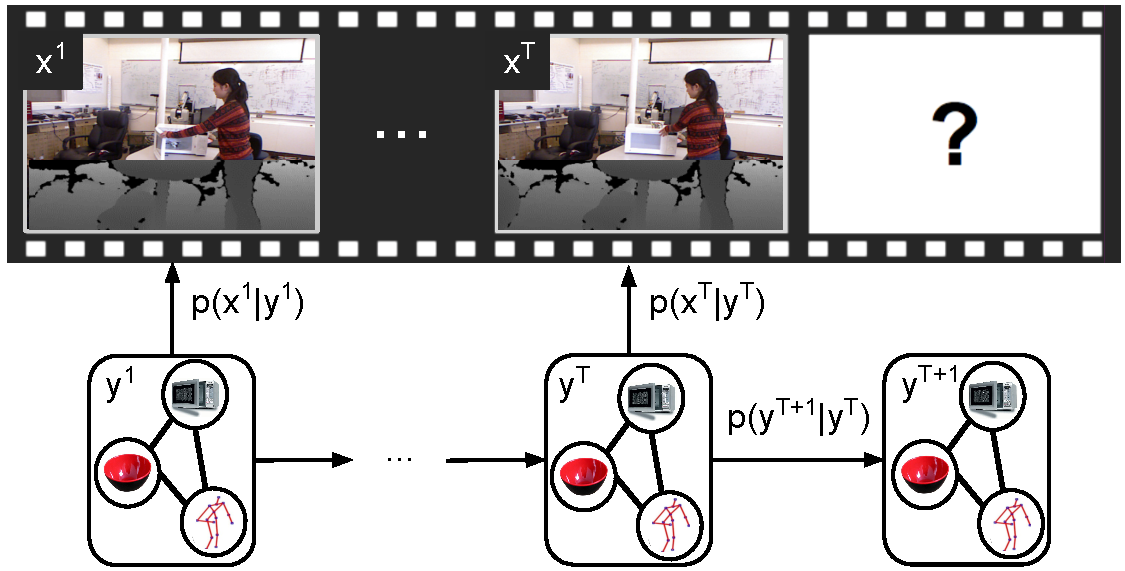
\includegraphics[width=\textwidth]{Fig1}
\caption{Figure is showing the state and measurements at each time represented by a CRF.
Our algorithm, rCRF, enables the application of recursive Bayesian estimation to CRF-based scene models. rCRF computes the full belief over human activity and object affordances ($y^1,\ldots,y^{T+M}$) by using RGB-D Video ($x^1,\ldots,x^T$).}
% In order to so, we propose a new model, rCRF, which can jointly use bayesian filtering and CRFs.}
%  which are not observed.}
%Estimating the belief over a CRF and using the estimated belief for anticipation and robot planning. \emph{(Colors of the nodes are representing the labels.)}}
\label{fig1}
\end{figure}

% modeling temporal evolution is still challenging in such a setting since the sampling procedure does not use temporal information \emph{(see Section~\ref{relwork} for mote details on this challenge)}.
Bayesian filtering methods can accurately estimate a belief (set of probabilities) over variables of interest from sequential data. However, it is still very challenging to estimate a belief over a CRF for two reasons. Firstly, it is not tractable to enumerate the labels over a CRF model since the output space has a dimension exponential in the number of objects, labels, and the temporal length\footnote{Typically with 10 objects, 10 min. length (with 1 sec. long segments), 10 activity and 10 object labels, dimension is $(10^{10}\times10)^{10\times60}=10^{6600}$.}. Secondly, there is a modelling difference between CRFs and Bayesian filtering framework. CRF is based on a discriminative setting whereas the Bayesian filtering mostly relies on the generative formulation.
% that requires the conditional probability of the observation given the variables of interest.
%where it models the conditional probability of the variables of interest given an observation,

In this chapter, we present a recursive algorithm -- Recursive CRF (rCRF) -- which can efficiently estimate a full belief over a CRF-based temporal scene model. rCRF can be seen as an efficient belief estimation method which enables us to use CRF-based scene model in Bayesian filtering. It models the temporal evolution via Bayesian updates and models the measurements in the scene via CRF. In order to use CRFs in such a scenario, we solve two problems. First, we present an approximation to convert the discriminative likelihood of the CRF into a generative measurement equation. Second, we use structured diversity for tractable computation. To the best of our knowledge, rCRF is the only tractable method that can use a CRF-based scene model in a recursive Bayesian filtering.
%Since we define the belief function recursively, we iterate the message propagation and diverse sampling until the convergence.

We apply the rCRF to the problem of activity detection and anticipation from RGB-D data. As a CRF-based scene model, we use the model from \cite{hemaIJRR} which represents the scene as a CRF over human activity and object affordances. We then use the RGB-D video to detect and anticipate activities via rCRF. %We use the rCRF framework in order to anticipate the future activities as well.

Our experiments show that we outperform the state-of-the-art methods for detection and anticipation, and the improvement in the anticipation accuracy is significant. In addition to the improvements in accuracy, we show that our anticipation also improves the computation time and runs near real-time.

%We believe that the presented efficient and accurate estimation of a full belief can be combined with an optimal decision mechanisms (e.g. minimum Bayes risk \cite{decisionTheory,nabbe2007extending}) for better assitive robots.

In summary, the contributions of this work are:
\begin{itemize}
\item  We present Recursive-CRF (rCRF) method that uses the rich modeling power of CRF in
Bayesian filtering setting.
%  allows CRF-based scene models in a Bayesian filtering.
% \item  We present a recursive method in order to estimate the full belief over an rCRF.
\item  We present a structured-diversity based approach to enable tractable computation of the belief.
\item  We apply our rCRF method to the problem of activity detection and anticipation in
RGB-D videos.
%\item  Our experiments show that rCRF significantly outperforms the state-of-the-art methods, both in accuracy and inference time.
\end{itemize}


% !TEX root = ../../ozan_sener_thesis.tex
\section{Related Work on Graphical Models for Robot Perception}
\label{relwork}
%\vspace{\sectionReduceTop}
%\vspace{1mm}
\noindent
{\bf Bayesian Recursive Filtering:}
\label{parf}
Estimating a belief over variables of interest from partial observations is a widely studied problem \cite{thrunBook}. Sequential Monte Carlo (SMC) ---aka \emph{particle filter}--- is typically used to estimate beliefs in high-dimensional cases. SMC methods represent the belief as a set of samples and we refer the reader to \cite{meanFieldBook} for rigorous analysis.

SMC methods are not directly applicable to spaces like CRF since the number of samples required is intractably high. One solution to this problem is the Rao-Blackwellised particle filter \cite{raob}. It uses a partition of the state variables $\bf{y}$ into two set of variables $\bf{y}_1$ and $\bf{y}_2$ such that the variables in one partition $\bf{y}_2$ can be estimated using the partition $\bf{y}_1$. Then Rao-Blackwellised particle filter \cite{raob} estimates the $\bf{y}_1$ via SMC and directly estimates $\bf{y}_2$ using $\bf{y}_1$. However, for our problem, we are not aware of any state decomposition which enables Rao-Blackwellised particle filter. Although there are discrimantive extensions of Bayesian models like recursive least squares\cite{sarkka}, in this chapter we only consider the states represented by CRFs. Moreover, we are not aware of any Bayesian smoothing formulation applied over CRFs.

One tractable application of the SMC framework to the CRF based scene analysis problems is the ATCRF \cite{hemaAnt} model. ATCRF \cite{hemaAnt} uses a set of heuristics to sample the particles. However, ATCRF faces the problem of computational limitations and requires computationally intractable number of samples for anticipation. We follow the Bayesian filtering theory and efficiently estimate the belief.

%\vspace{2mm}
\noindent
{\bf Structured Diversity and Variants of CRFs:}
CRFs are widely used to solve activity analysis problems \cite{siminchi2005,quattoni2007} in a discriminative setting. CRF models the conditional likelihood of the state given the observations, and the MAP solution can be found. Although this setting is powerful, it does not give any information about the belief other than the MAP state.

Other than the MAP solution, it is also tractable to compute the modes of the CRF \cite{divmbest,mbest,mmode}. These modes can be considered as an approximate state space, and the belief can be computed only for them. Indeed, this claim is empirically validated in many problems like parameter learning \cite{mlparam}, empirical MBR \cite{embr} and discrimantive re-ranking \cite{rerank}.

Among the aforementioned approaches, Div-M-Best \cite{divmbest} is a method applicable to the sequential information. \cite{divmbest} starts by dividing the video into a set of frames and computes the diverse-most-likely solutions of each frame independently. Then, it combines the results via the temporal relations. On the contrary, we formulate the problem as recursive Bayesian smoothing and compute the samples based on temporal relations. Formally, given state variables $\mathbf{y}^1,\ldots,\mathbf{y}^T$ and observations $\mathbf{x}^1,\ldots,\mathbf{x}^T$, we directly sample $p(\mathbf{y}^t|\mathbf{x}^1,\ldots,\mathbf{x}^T)$, whereas, \cite{divmbest} samples $p(\mathbf{y}^t|\mathbf{x}^t)$. Since our sampling procedure uses the entire video, our samples are more accurate.

There are variants of CRFs that rely on sequential models as well such as, Dynamic CRF (dCRF) \cite{dcrf}, Infinite Hidden CRF \cite{ihcrf}, Gaussian Process Latent CRF \cite{gpcrf} and Hierarchical Semi-Markov CRF (HSCRF). Although they are applicable to videos, we are not aware of any tractable method to compute a belief over any of the aforementioned graphical model.

DCRF \cite{ddcrf} learns the observation likelihood --$p(\mathbf{x^t}|\mathbf{y^t})$-- by using the low-dimensional nature of the features and follows Bayesian filtering. Since our features have very high-dimension (for $N$ objects, we have $58N+20N^2+103$ dimensional features), DCRF \cite{ddcrf} is not directly applicable. However, it is possible to learn $p(\mathbf{y^t}|\mathbf{x^t})$ and \emph{approximately} use the DCRF formulation by assuming observation and label likelihoods are equal. Moreover, This approach can be shown equivalent to finding local maximum of energy function defined by \cite{hemaIJRR} following the formulation of Fox et al \cite{foxThesis}.

It is also common to compute a belief over latent nodes as in the case of infinte hidden CRF \cite{ihcrf} and Gaussian Process Latent CRF\cite{gpcrf}. However, they are not directly applicable to our problem since they can compute a belief only over the latent node. CRF-Filter \cite{crffilter} is a closely related approach which uses CRFs in a particle filtering scenario. However, it is based on sampling of a low dimensional state space and it is not applicable to our rich model either.

%\vspace{2mm}
\noindent
{\bf Human Activity Detection and Anticipation:} Early works relied solely on human poses. These works range from jointly segmenting and recognizing sub-activities \cite{hoai2011,shi2011} to choosing a relevant model out of activity models \cite{pyry2012}. Main limitation of these methods is that they do not use the object information. Some methods successfully model and use the relations of the human-poses and objects in the scene \cite{davis2009,feifei2010,jiang2012,hall}. However, a significant drawback of these works is missing the fact that object affordance is more important than object types for activities \cite{gibson1979}. Indeed, object affordance based models had higher performance (e.g., \cite{hemaIJRR}). A recent work modelled human activities with latent models \cite{latentIcra} and also handled the disagreements among the activity annotations \cite{rss2014}.

Another drawback of these methods is the requirement of the entire activity. Detecting the activity in its early stages is especially crucial for assistive robotics and surveillance systems. Although a few recent work adress the problem of activity detection with partial/early information \cite{torre2012,ryoo2011}, these works do not perform anticipation. There are a few recent works addressing \emph{what human will perform next} by using trajectory prediction. It is possible to predict the trajectory of the human  using inverse reinforcement learning in 2D \cite{ziebart2009,kuderer2012,kitani2012} or 3D \cite{dragan2012}. However, these models rely on the low-dimensional structure of the 2D/3D coordinate space and therefore they do not apply to rich models like CRF.

Recent work on anticipatory temporal CRF \cite{hemaAnt} considers an anticipation with a CRF model. It anticipates the future via augmenting set of possible future observations to the CRF. It is also extended with an improved human motion model based on a Gaussian process \cite{gpcrf}. However, their accuracy significantly drops for a long anticipation horizon since they fail to represent the uncertainty. Our method overcomes these problems by recursively estimating a full belief.
%\vspace{\sectionReduceBot}



\section{Overview}
\label{overview}
\begin{figure}[t]
  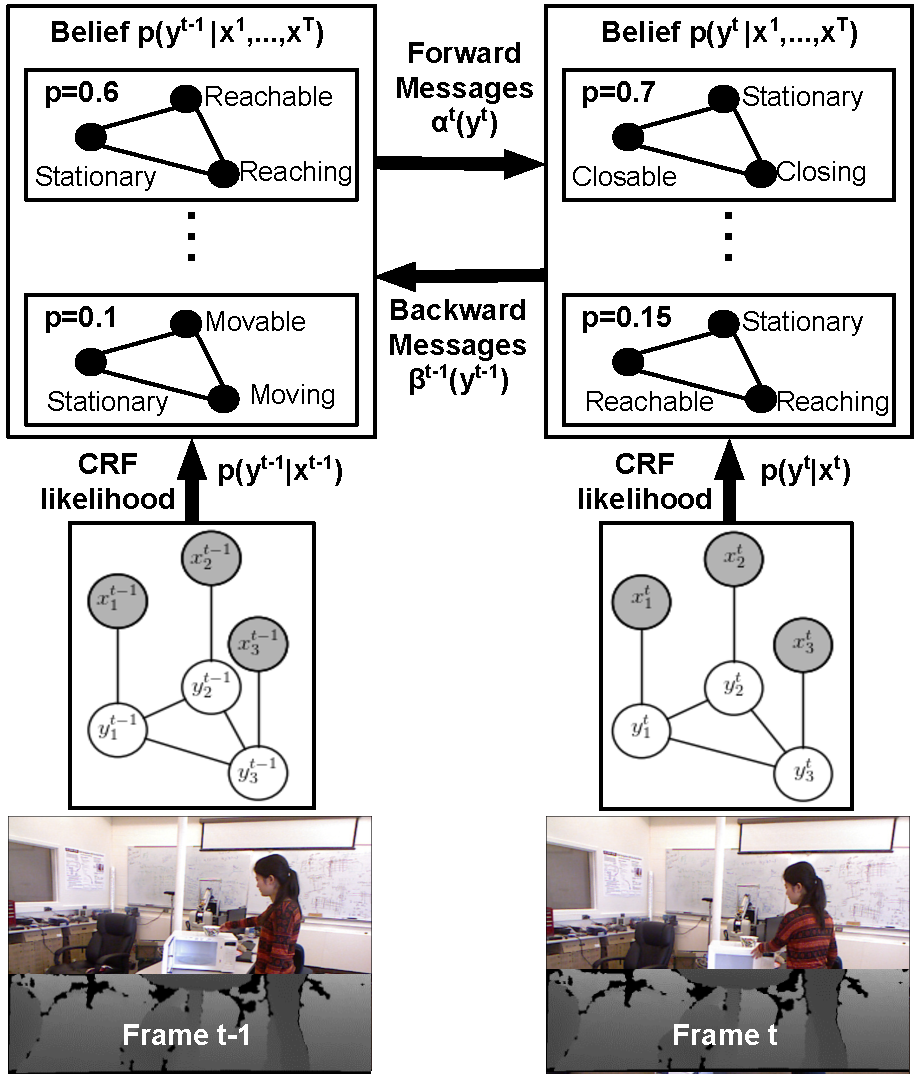
\includegraphics[width=\textwidth]{systemflow}
  \caption{{\bf Computing the full belief by using rCRF.} Each iteration of the recursive estimation algorithm includes computing forward and backward messages, $\alpha^t(\mathbf{y}^t)$ and $\beta^{t-1}(\mathbf{y}^{t-1})$, by using the current samples and computing the belief $p(\mathbf{y}^t|\mathbf{x}^1,\ldots,\mathbf{x}^T)$ with the computed messages. Then, we re-compute the messages and re-sample the belief until the belief converges. \emph{Here, we only have two objects as  $\mathbf{y}^t=(\mathbf{O}^t_1,\mathbf{O}^t_2,\mathbf{A}^t)$ and $\mathbf{x}^t=(\mathbf{L}^t_1,\mathbf{L}^t_2,\mathbf{H}^t)$ }}
  \label{system}
\end{figure}
%Toy Example
In this section, we summarize our method and explain how we estimate the full belief over the activities and object affordances. Moreover, we also give an illustrative example of the rCRF with a toy scene consisting of two objects (a microwave and a bowl) and a human in Figure~\ref{system}.

%CRF
Reasoning about activities requires not only identifying the objects but also interpreting object-object relations and human-object relations. Indeed, we capture such rich information via CRF. As shown in the Figure~\ref{system}, each object and a human corresponds to a node in the graph on which we define the CRF. As a hidden variable, we are interested in object affordances such as \emph{openable, graspable, movable, etc.}, and the activity human is performing such as \emph{moving, opening, grasping, etc.}. We define the affordances as the actions that can be performed on/with the object~\cite{gibson1979}. We denote the affordance variables at time $t$ as $\mathbf{O}^t_1, \ldots, \mathbf{O}^t_N$ for $N$ objects and the activity variable as $\mathbf{A}^t$. Since they are not directly observed, we estimate them by using partial observations. We are using the 3D positions of the objects $\mathbf{L}^t_1,\ldots,\mathbf{L}^t_N$ and the human pose $\mathbf{H}^t$ as observations. %Human pose corresponds to the 3D position of the joints of the human in the scene.
The input video is temporally over-segmented prior to the application of the belief estimation, and the time instant $t$ represent the $t^{th}$ segment of the video. We explain the features and the potential functions we use while defining the CRF in Section~\ref{rgbd}.

In addition to the spatial relations between objects and humans, we are also interested in their temporal evolution. In general, the problem of estimating a belief over set of hidden variables using the entire video corresponds to a Bayesian smoothing problem. Formally, we are interested in estimating states \mbox{$\mathbf{y}^t=(\mathbf{O}_1^t,\ldots,\mathbf{O}_N^t,\mathbf{A}^t)$} given set of observations \mbox{$\mathbf{x}^t=(\mathbf{L}_1^t,\ldots,\mathbf{L}_N^t,\mathbf{H}^t)$}. We estimate the states through successive application of the recursive Bayesian updates. In order to tractably compute the Bayesian updates, we introduce two approximations in Section~\ref{theory}. First, we compute the set of all plausible future states by using structured-diversity. Second, we use Jensen inequality in order to convert the discriminative likelihood into a generative one. After the introduction of these two machineries, we follow the recursive Bayesian estimation framework. As shown in Figure~\ref{system}, we first compute the Bayesian updates through the forward and backward messages, $\alpha^t(\mathbf{y}^t)$ and $\beta^{t}(\mathbf{y}^{t})$. We then compute the posterior belief $p(\mathbf{y}^t|\mathbf{x}^1,\ldots,\mathbf{x}^T)$ by using the computed messages and the CRF-likelihood \emph{$p(\mathbf{y}^t|\mathbf{x}^t)$}. As a final step of the iteration, we represent the belief via diverse samples of the posterior belief. Since the belief is recursively defined, we re-compute the messages and re-sample the belief until it converges.

%We denote the observation as $\bf{x^t}$ and the hidden state as $\bf{y^t}$ for clarity. After defining the rCRF and developing the algorithm in Section~\ref{theory}, we return to the problem of activity analysis and its notation in Section~\ref{rgbd}.

% !TEX root = ../../ozan_sener_thesis.tex
\section{Belief Estimation with  rCRF}
\label{theory}
In this section, we develop the Recursive Conditional Random Field (rCRF) to use CRF in a Bayesian filtering setting. rCRF jointly uses rich model of CRF and the recursive nature of the Bayesian filtering to compute an accurate belief. We first define our modelling assumptions in Section~\ref{rcrfdef}, and then we introduce a link between the CRF likelihood and the measurement likelihood in Section~\ref{fromto} in order to compute the posterior belief. In Section~\ref{beliscrf}, we further show that the resulting posterior belief is equivalent to a CRF. Moreover, this equivalence enables efficient computation via the diversity based method \cite{divmbest} developed for CRFs.
\subsection{Recursive Conditional Random Field}
\label{rcrfdef}
Consider a sequential estimation problem in which we are interested in variables $\mathbf{y}^t$ using observations $\mathbf{x}^t$ where $t$ is the temporal variable. In our application, $t$ is the temporal segment id. We note RGB-D camera reading as $\mathbf{x}^t$, and object and activity labels as $\mathbf{y}^t$. We now define the Recursive Conditional Random Field (rCRF) framework for such a problem following the assumptions of Hidden Markov Models.

\begin{mydef}
Let $\mathcal{G}^t=(V^t,E^t)$ be set of graphs indexed by the temporal variable $t$ and $\mathbf{y}^t$ is indexed by the vertices of $\mathcal{G}^t$ as $\mathbf{y}^t=(y^t_v)_{v \in V^t}$. Then, ($\mathbf{x}^{1\ldots T}$,$\mathbf{y}^{1\ldots T}$) is a \textbf{\textit{Recursive Conditional Random Field}} with dynamics $p_v(\cdot|\cdot)$ when

\begin{enumerate}
	\item For each $t$, $(\mathbf{y}^t,\mathbf{x}^t)$ is a CRF over $\mathcal{G}^t=(V^t,E^t)$
%	\item $\mathbf{y^t} \perp \mathbf{y^{t-k}} | {\mathbf{y^{t-1}}} \quad  \forall {k>1}$
\item $p(\mathbf{y}^{t}|\mathbf{y}^{1},\ldots,\mathbf{y}^{t-1}) = p(\mathbf{y}^{t}|\mathbf{y}^{t-1}) \quad  \forall t$ \hfill (Markov)
%\mathbf{y^{t+1}} \perp \mathbf{y^{t-1}} \; | \; {\mathbf{y^{t}}} \quad  \forall t$ \hfill (Markov)
%	\item $\mathbf{y^{t+1}} \perp \mathbf{y^{t-1}} \; | \; {\mathbf{y^{t}}} \quad  \forall t$ \hfill (Markov)
\item $p(\mathbf{x}^t|\mathbf{y}^1,\ldots,\mathbf{y}^t,\mathbf{x}^1,\ldots,\mathbf{x}^{t-1})=p(\mathbf{x}^t|\mathbf{y}^t)\quad  \forall t$ \hfill
%\item $\mathbf{x^t} \perp \mathbf{y^u} | \mathbf{y^t} \quad  \forall {u \neq t}$ \hfill (Measurements are Cond.Ind.)
\item $p(\mathbf{y}^t=\mathbf{y}|\mathbf{y}^{t-1}=\mathbf{y^\prime})=p_v(\mathbf{y}|\mathbf{y^\prime})$ \hfill (stationarity)
\end{enumerate}
$\hfill \blacksquare$
\end{mydef}
\begin{figure}[ht]
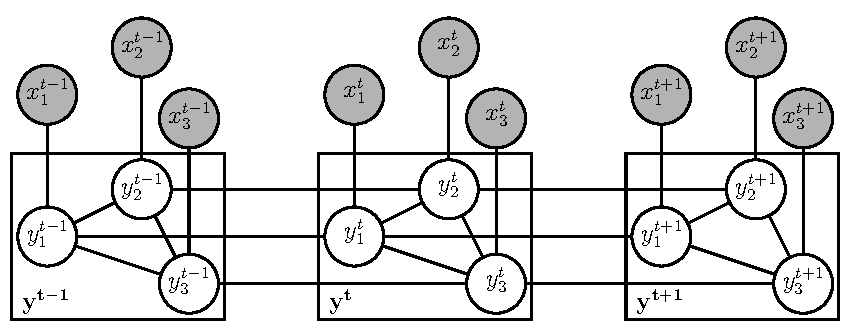
\includegraphics[width=\textwidth]{hmmcrf}
\caption{{\bf rCRF is defined over a temporal CRF.} The graphical model, we use within the rCRF, is a temporal CRF with additional constraints. We impose a special structure through the conditions we state in the definition. For the visualization purposes, we show there nodes per segment although rCRF can handle any number of nodes.}% Shaded nodes represent the observations.
\label{rCrf}
\end{figure}

We visualize the graphical model representation of the rCRF in Figure \ref{rCrf}. In this work, we are interested in the belief over state variables at a given time instant $t$ as:
\begin{equation}
bel^t(\mathbf{y}) = p(\mathbf{y}^t=\mathbf{y}|\mathbf{x}_1,\ldots,\mathbf{x}_T) \label{beldef}
\end{equation}
Here, $T$ denotes the length of the video. Hence, in rCRF the belief of any frame is supported by the entire video. Moreover, the time instant $t$ can be greater than the video length $T$ as well. Hence, rCRF naturally supports anticipation setting.
% This problem is typically referred as Bayesian smoothing.

We then decompose the belief by using the independence properties of the rCRF as:
\begin{equation}
bel^t(\mathbf{y}) \propto  \underbrace{p(\mathbf{y}^t=\mathbf{y}|\mathbf{x}^1,\ldots,\mathbf{x}^t)}_{\alpha^t(\mathbf{y})} \underbrace{p(\mathbf{x}^{t+1},\ldots,\mathbf{x}^T|\mathbf{y}^t=\mathbf{y})}_{\beta^t(\mathbf{y})}
\label{beldec}
\end{equation}
Moreover, $\alpha^t$ and $\beta^t$ can be computed recursively by using forward and backward  messages. Following \cite{hmm},
\begin{equation}
\begin{aligned}
\alpha^t(\mathbf{y}^t) &= p(\mathbf{x}^t|\mathbf{y}^t)\sum_{\mathbf{y}^{t-1}} \alpha^{t-1}(\mathbf{y}^{t-1}) p(\mathbf{y}^{t}|\mathbf{y}^{t-1}) \\
\beta^t(\mathbf{y}^t) &= \sum_{\mathbf{y}^{t+1}} p(\mathbf{x}^{t+1}|\mathbf{y}^{t+1}) \beta^{t+1}(\mathbf{y}^{t+1}) p(\mathbf{y}^{t+1}|\mathbf{y}^{t})
\end{aligned}
\label{mespas}
\end{equation}
\noindent
with initializations $\alpha^1(\mathbf{y}^1)=p(\mathbf{x}^1|\mathbf{y}^1)$ and $\beta^T(\mathbf{y}^T)=1$.

\subsection{Computing the belief using an rCRF}
\label{fromto}
Recursive definition in (\ref{mespas}) has two significant drawbacks:
 firstly, CRF is modelling $p(\mathbf{y}^t|\mathbf{x}^t)$ instead of $p(\mathbf{x}^t|\mathbf{y}^t)$ and the transformation is not trivial. Secondly, computation of the messages require a summation over the entire output space, and it has an exponential dimension. In this section, we first compute the posterior of the observation given labels $p(\mathbf{x}^t|\mathbf{y}^t)$ by using the CRF posterior likelihood $p(\mathbf{y}^t|\mathbf{x}^t)$. Then, we show that the belief function at time $t$, $bel^t(\mathbf{y})$, can be approximately represented as a Gibbs measure over $\mathcal{G}^t$. Then, we conclude that the belief, $bel^t(\mathbf{y})$, is a CRF over the graph $\mathcal{G}^t$ with modified energy functions.
%Finally, we suggest a method to efficiently represent the belief over small number of samples in section \ref{divm}.
\subsubsection{From $p(\mathbf{y}^t|\mathbf{x}^t)$ to $p(\mathbf{x}^t|\mathbf{y}^t)$}
Since $(\mathbf{x}^t,\mathbf{y}^t)$ is a CRF, the posterior of the label given the observation follows \cite{geman}; %a Gibbs measure \cite{geman} as;
\begin{equation}
p(\mathbf{y}^t|\mathbf{x}^t) \propto \exp\left( \sum_{i \in V^t} \theta_{x^t_i}(y^t_i) + \sum_{i,j \in E^t} \theta_{x^t_i,x^t_j}(y^t_i,y^t_j)  \right)
\label{crflogl}
\end{equation}
where $\theta$ is the energy function defined over the node set \mbox{$v \in V^t$ }as $\theta_{v}$ and over the edge set \mbox{$(u,v) \in E^t$} as $\theta_{u,v}$.

%\frac{p(\mathbf{y}^t|\mathbf{x}^t)}{p(\mathbf{y}^t)} =
In order to transform  $p(\mathbf{y}^t|\mathbf{x}^t)$ into  $p(\mathbf{x}^t|\mathbf{y}^t)$, we use Bayes rule;
$p(\mathbf{x}^t|\mathbf{y}^t) \propto  \frac{p(\mathbf{y}^t|\mathbf{x}^t)}{ \sum_{x^t} p(\mathbf{y}^t|\mathbf{x}^t)p(\mathbf{x}^t)}$ and compute $p(\mathbf{y}^t)$ as; %the denominator as;
\begin{equation}
p(\mathbf{y}^t)=\sum_{\mathbf{x}^t} \exp\left( \sum_{i \in V^t} \theta_{x^t_i}(y^t_i) + \sum_{i,j \in E^t} \theta_{x^t_i,x^t_j}(y^t_i,y^t_j) \right) p(\mathbf{x}^t)
\end{equation}
For tractability, we approximate the $p(\mathbf{y}^t)$ with its lower bound after applying the Jensen inequality as;
\begin{equation}
	\small
p(\mathbf{y}^t) \approx \exp ( \sum_{i \in V^t} \underbrace{\sum_{\mathbf{x}^t} \theta_{x^t_i}(y^t_i)  p(\mathbf{x}^t)}_{\tilde{\theta}(y^t_i)} + \sum_{i,j \in E^t} \underbrace{ \sum_{\mathbf{x}^t}  \theta_{x^t_i,x^t_j}(y^t_i,y^t_j) p(\mathbf{x}^t)}_{\tilde{\theta}(y^t_i,y^t_j)} )
\end{equation}

% \todo{
We then estimate the inner summations $\tilde{\theta}(\cdot)$
% , expectation over $\mathbf{x}$, )
% empirically by
from the training data
% In other words, we
using Monte Carlo method
% to compute inner summations
 as \mbox{$\tilde{\theta}(\cdot) = \frac{1}{N}\sum_{i=1}^N \theta_{\mathbf{x}^{(i)}}(\cdot)$} where $N$ is the number of training samples and $\mathbf{x}^{(i)}$ is the $i^{th}$ training sample.
 %  with abuse of notation.
 Therefore, we can compute the observation likelihood as:  $p(\mathbf{x}^t|\mathbf{y}^t) \propto$
\begin{equation}\small
\exp\left( \sum_{i \in V^t} \theta_{x^t_i}(y^t_i) - \tilde{\theta}(y^t_i) + \sum_{i,j \in E^t} \theta_{x^t_i,x^t_j}(y^t_i,y^t_j) - \tilde{\theta}(y^t_i,y^t_j)  \right)
\label{obsprob}
\end{equation}

\subsubsection{Belief is a CRF}
\label{beliscrf}
Here we compute the belief (\ref{beldec}) in terms of forward and backward messages and CRF likelihood. We then show that the posterior belief is a CRF. This observation enables us to use efficient methods developed for CRFs.

In order to compute the belief (\ref{beldec}), we decompose
% assume that
% start with the simplifying assumption that
the system dynamics using the independence assumption in the graph in Fig.~\ref{rCrf}.
This gives us \mbox{$p(\mathbf{y}^t|\mathbf{y}^{t-1})=\prod_{i} p(y^t_i|y^{t-1}_i)$}.
% In other words, the system dynamics model does not model correlations
%
% we model the relationship between variables via CRF and do not consider them while modelling temporal dynamics.
%
%After decomposing the state transition dynamics,
We then compute the belief function as \mbox{$bel(\mathbf{y}^t)=\alpha^t(\mathbf{y}^t)\beta^t(\mathbf{y}^t)$} by using equations (\ref{mespas}) and (\ref{obsprob}). After algebraic manipulations, the belief function can be approximated as follows (see supplementary material for a detailed derivation):
\iffalse
\begin{equation}\small
	\begin{aligned}
&bel(\mathbf{y}^t) \propto \exp\left[  \sum_{i,j \in E^t} \left( \theta_{x^t_i,x^t_j}(y^t_i,y^t_j) - \tilde{\theta}(y^t_i,y^t_j) \right) \right. \\
&\left. \sum_{i \in V^t} \left( \theta_{x^t_i}(y^t_i) - \tilde{\theta}(y^t_i) +  \sum_{\mathbf{y^{t-1}}} \alpha^{t-1}(\mathbf{y}^{t-1}) \log p(y^t_i|y^{t-1}_i) \right. \right. \\
&+\left.\left.\sum_{\mathbf{y}^{t+1}} \beta^{t+1}(\mathbf{y}^{t+1}) p(\mathbf{x}^{t+1}|\mathbf{y}^{t+1}) \log p(y^t_i|y^{t-1}_i) \right) \right]
\end{aligned}
\label{crfbelief}
\end{equation}
\fi

\begin{equation}\small
  \begin{aligned}
&bel(\mathbf{y}^t) \propto \exp\left[  \sum_{i,j \in E^t} \left( \theta_{x^t_i,x^t_j}(y^t_i,y^t_j) - \tilde{\theta}(y^t_i,y^t_j) \right) \right. \\
&\left. \sum_{i \in V^t} \left( \theta_{x^t_i}(y^t_i) - \tilde{\theta}(y^t_i) +  \sum_{\mathbf{y}^{t-1}} \alpha^{t-1}(\mathbf{y}^{t-1}) \log p(y^t_i|y^{t-1}_i) \right. \right. \\
&+\left.\left.\frac{1}{\gamma}\sum_{\mathbf{y}^{t+1}} \beta^{t+1}(\mathbf{y}^{t+1}) p(\mathbf{x}^{t+1}|\mathbf{y}^{t+1}) \log p(y^{t+1}_i|y^{t}_i) \right) \right]
\end{aligned}
\label{crfbelief}
\end{equation}
where $\gamma=\sum_{\mathbf{y}^{t+1}} \beta^{t+1}(\mathbf{y}^{t+1}) p(\mathbf{x}^{t+1}|\mathbf{y}^{t+1})$

One property to observe is the decomposition of the belief over the graph. Resulting belief function, (\ref{crfbelief}), is a summation over energy terms defined over nodes $i \in V^t$ and edges $i,j\in E^t$. Hence, belief $bel^t(\cdot)$ is a Gibbs measure over $\mathcal{G}^t$. By using Hammersley-Clifford theorem \cite{hc1971}, we  conclude that the posterior belief in rCRF is also a CRF. In other words, belief is a CRF defined over the same graph with a modified energy.

\subsubsection{Belief via Diverse-Most-Likely Samples}
\label{divm}
Since we computed the belief function and showed that it is equivalent to a CRF, we now need
an efficient method for computing it.

% here we use an existing method, computing diverse-most-likely samples \cite{divmbest}, that is developed for a CRF, in order to efficiently compute the belief.

We follow the observation that CRF-likelihood over a natural scene concentrates on a few diverse samples \cite{divmbest} because each scene only has a few plausible explanation. So, we compute the belief for only those samples. In other words, let's assume the set of all plausible solutions at time $t$ is $\mathbf{Y}^t={\mathbf{y}^{t,1},\ldots,\mathbf{y}^{t,M}}$ where $\mathbf{y}^{t,i}$ is the $i^{th}$ sample at time $t$. We then redefine the belief as;

\begin{equation}
	\text{approx\_bel}^t(\mathbf{y})=\left\{ \begin{array}{cc} \frac{bel^t(\mathbf{y})}{\sum_{\mathbf{y}^\prime \in \mathbf{Y}^t} bel^t(\mathbf{y}^\prime)} & \text{if $\mathbf{y} \in \mathbf{Y}^t$} \\ 0 & \text{o.w.} \end{array} \right.
\end{equation}

Since there are only a few plausible explanation of a visual observation and CRF-based belief concentrates only on those samples, proper selection of the samples $\mathbf{Y}^t$ is expected to work well in practice. These samples are typically selected as the diverse-most-likely solutions of the CRF. They are most-likely samples because we are only interested in the plausible explanations. They are diverse because we are interested in the modes of the CRF other than set of samples around the MAP solution. Diversity is achieved via asserting samples to be at least $\delta$ unit apart from each other via the distance function $\Delta$ (we use hamming distance as a in our experiments). In other words, we solve the following optimization problem in order to get the samples which represent the belief;
\begin{equation}
\begin{aligned}
\mathbf{y}^{t,i} &= \argmax_{\mathbf{y}}  bel^t(\mathbf{y}) \\
&s.t.\,\, \Delta(\mathbf{y},\mathbf{y}^{t,j}) \geq \delta \quad \forall \; {j < i}
\end{aligned}
\label{divopt}
\end{equation}
%where $\bf{y}^{t,i}$ is the $i^{th}$ sample in the $t^{th}$ frame.
This optimization is NP-hard in general; however, since we already showed $bel^t(\bf{y})$ is CRF, we use the existing diverse-m-best algorithms developed for CRFs. We use the Lagrange relaxation by Batra et al. \cite{divmbest}. We explain the details of solving this problem by using \cite{divmbest} in supplementary material.

In summary, we first compute the belief via (\ref{crfbelief}) for all frames by using samples of the previous and the next frame as well as CRF likelihoods. Then, we compute the diverse samples of (\ref{crfbelief}) by using \cite{divmbest}. After computing the samples, we compute the messages $\alpha^t$ and $\beta^t$ by using the equations (\ref{obsprob}) and (\ref{mespas}). We continue to re-sample the beliefs and re-compute the messages recursively until the convergence. Moreover, during the initialization, we only sample the observation function (\ref{obsprob}) since the messages are not available.

% !TEX root = anticipation_divmrf.tex
\section{Human Activity Detection and Anticipation}
\label{rgbd}
In this section, we describe how we apply the rCRF framework to RGB-D videos for human activity detection and anticipation. We are interested in activities such as \emph{reaching} and \emph{moving}, and object affordances such as \emph{reachable} and \emph{movable} as explained in Section~\ref{overview}. We follow the approach in \cite{hemaIJRR}, and start with temporally segmenting the video. This step can be considered as an oversegmentation in the temporal domain. It decreases the computation complexity and enables using motion information as an observation.

We then obtain the observations $\mathbf{x}^t=(L_1^t,L_2^t,H^t)$, by detecting the objects in the first frame and then tracking them. We obtain the human pose $H^t$ through a skeleton tracker. We consider affordances and activities as state \mbox{$\mathbf{y}^t=(O^t_1,\ldots,O^t_N,A)$} where $N$ is the number of objects. We extracted set of features from the observations following the feature functions in \cite{hemaIJRR} (\emph{eg.} relative and absolute location of objects, human joints and their temporal displacements). After extracting the features, we define our CRF as a log-linear CRF and learn the energy function defined in (\ref{crflogl}) by using the Structural SVM \cite{ssvm} as in the case of \cite{hemaIJRR}. We use the first order statistics for temporal dynamics as \mbox{$p_v(y,y^\prime)=p(Y^t_v=y|Y^{t-1}_v=y^\prime)=\frac{\#(Y^t_v=y,Y^{t-1}_v=y^\prime)}{\#(Y^t_v=y\prime)}$} where $\#(\cdot,\cdot)$ is number of the co-occurrence in training data.

After defining the observation, state and dynamics, we apply the rCRF framework. We also summarize the activity detection and anticipation application in Algorithm~\ref{alg:recursive}.%\vspace{-5mm}

\setlength{\textfloatsep}{0.1pt}
\begin{algorithm}
\caption{Compute belief the over $(O^t_{1\ldots N},A^t)$ for \mbox{$t \in [1,T+\tau]$} in an RGB-D Video of length $T$}
\label{alg:recursive}
\begin{algorithmic}
\STATE {\bf Initialization:}
\STATE Compute $L^t_1,\ldots,L^t_N$, and $H^t$ for $t \in [1,T]$ via \cite{hemaIJRR}.
\STATE Compute $p(L^t_{1\ldots N},H^t|O^t_{1\ldots N},A^t)$ for $t \in [1,T]$ via (\ref{obsprob})
\STATE Compute the belief via (\ref{crfbelief}) w/o messages ($\alpha=1,\beta=1$)
\end{algorithmic}
\begin{algorithmic}
\STATE {\bf Detection:}
\REPEAT
\FOR {$t \in [1,T]$}
%\STATE Compute $p(L^t_{1\ldots K},H^t|O^t_{1\ldots K},A^t)$ via (\ref{obsprob})
\STATE Compute the forward/backward messages via (\ref{mespas})
\STATE Compute the belief via (\ref{crfbelief}) an sample via (\ref{divopt})
%\STATE Sample the posterior belief via (\ref{divopt})
\ENDFOR
\UNTIL convergence or number of iterations limit
\STATE {\bf Anticipation:}
\FOR {$t \in [T+1,T+\tau]$}
\STATE Compute only the forward messages via (\ref{mespas})
\STATE Sample the belief directly from the forward messages.
\ENDFOR
\end{algorithmic}
\end{algorithm}

%\vspace{-3mm}
%During the initialization stage in Algorithm~\ref{alg:recursive}, we compute the belief without messages since the recursive computation of the messages requires a belief. After the initialization, we apply the full rCRF algorithm recursively.

Moreover, since the temporal relations are modeled as causal, we do not compute the backward messages during the anticipation. In anticipation, there is also no future observation. Hence, the belief is defined solely by the forward messages. In order to compute the belief for future frames, we propagate the estimated belief. We propagate the belief to the next frame by sampling the next state of the each sample in the belief of the current frame via the temporal dynamics. Then, we choose diverse most likely samples out of the propagated samples via solving (\ref{divopt}) with exhaustive search.

% !TEX root = rCRF.tex
\section{Experimental Results}
In order to experimentally evaluate the proposed rCRF model and the belief computation, we perform experiments on two applications. Firstly, we estimate a belief over the activity a human is performing and the affordances of the objects in the scene by using the RGB-D video. After computing the belief, we detect the most likely activity and affordance sequences and study the improvement in the detection accuracy. Secondly, we test the accuracy of the beliefs in the anticipation setting. Indeed, we show that it is possible to obtain high-quality detection and anticipation via rCRF.

\begin{figure}[ht]
\small
%\begin{singlespace}
\begin{tabular}{p{5mm}@{}l}
\begin{tabular}{r}
\rotatebox[origin=r]{90}{\;\;\;\;\;\;\;Middle Frame}\\
\rotatebox[origin=l]{90}{Belief\;\;\;\;\;\;\;}
\end{tabular}
&
\begin{tabular}{p{3.7cm}p{3.7cm}p{3.7cm}p{3.7cm}}
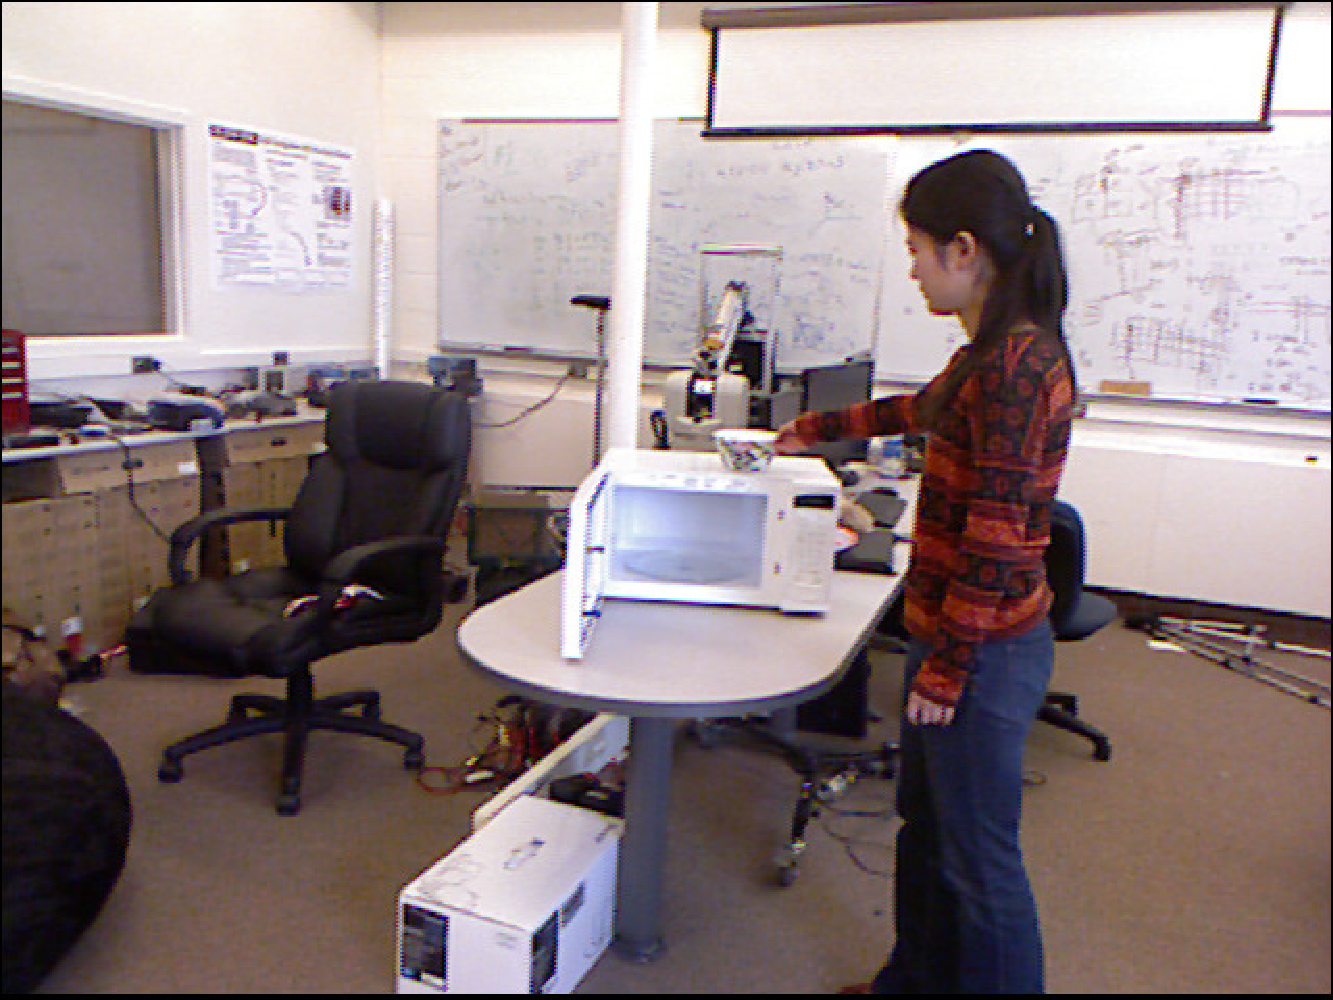
\includegraphics[width=0.225\textwidth]{f10} &
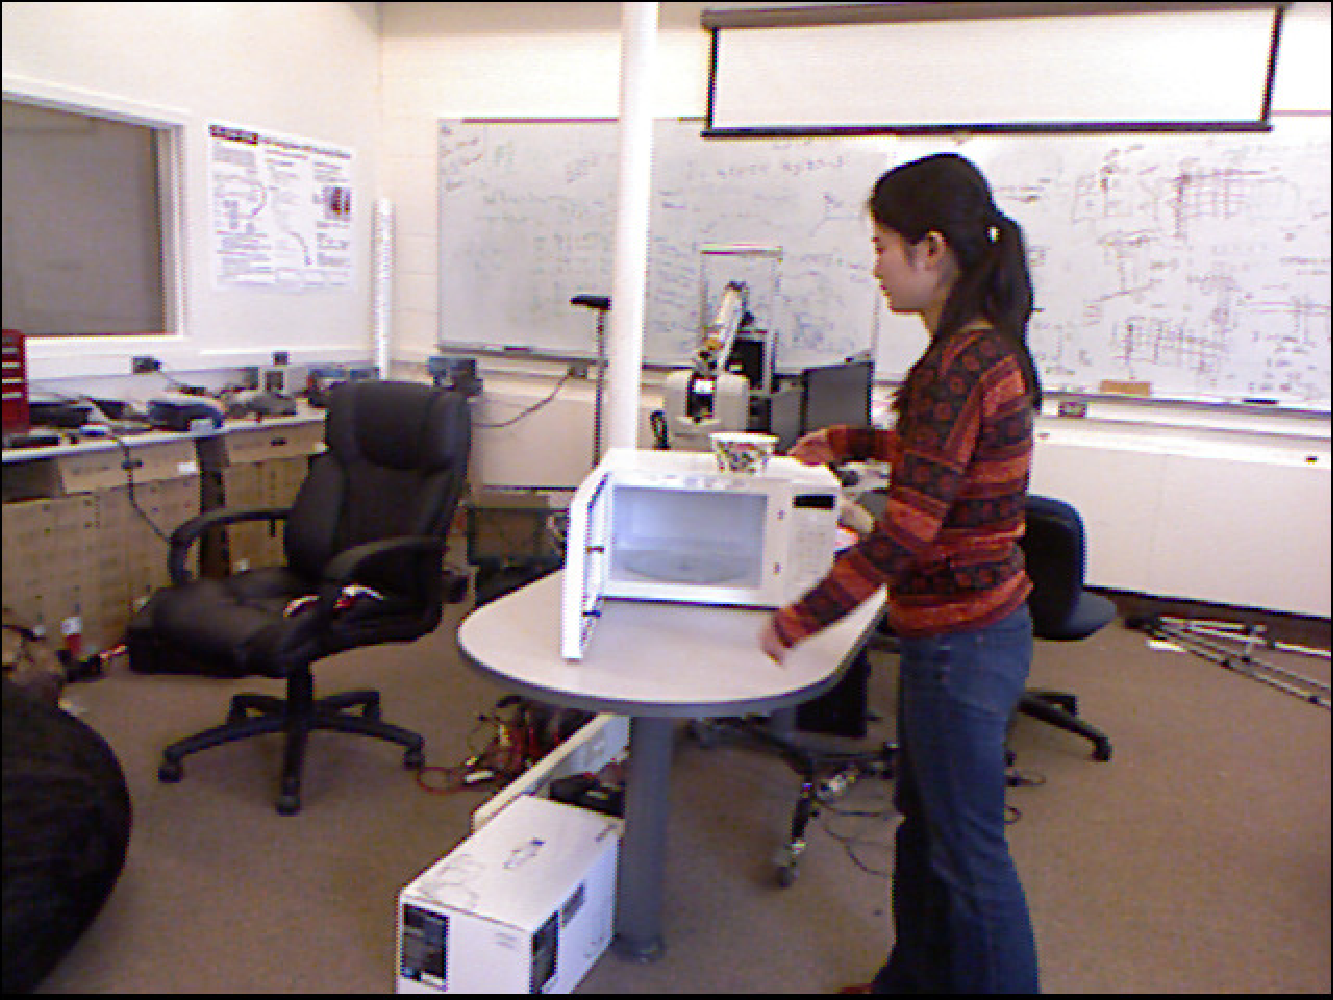
\includegraphics[width=0.225\textwidth]{f11} &
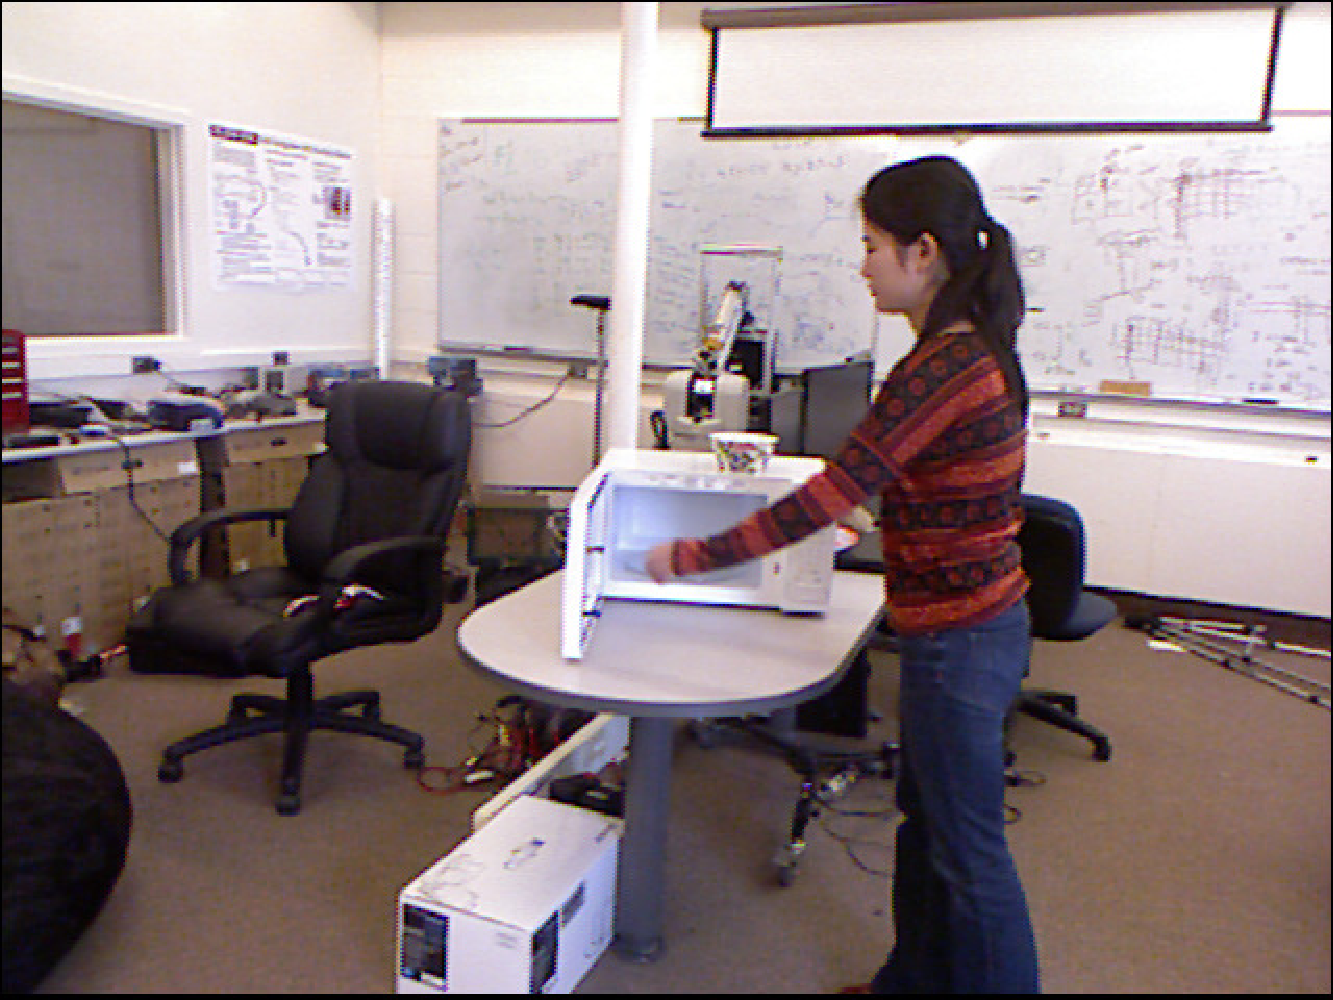
\includegraphics[width=0.225\textwidth]{f12} &
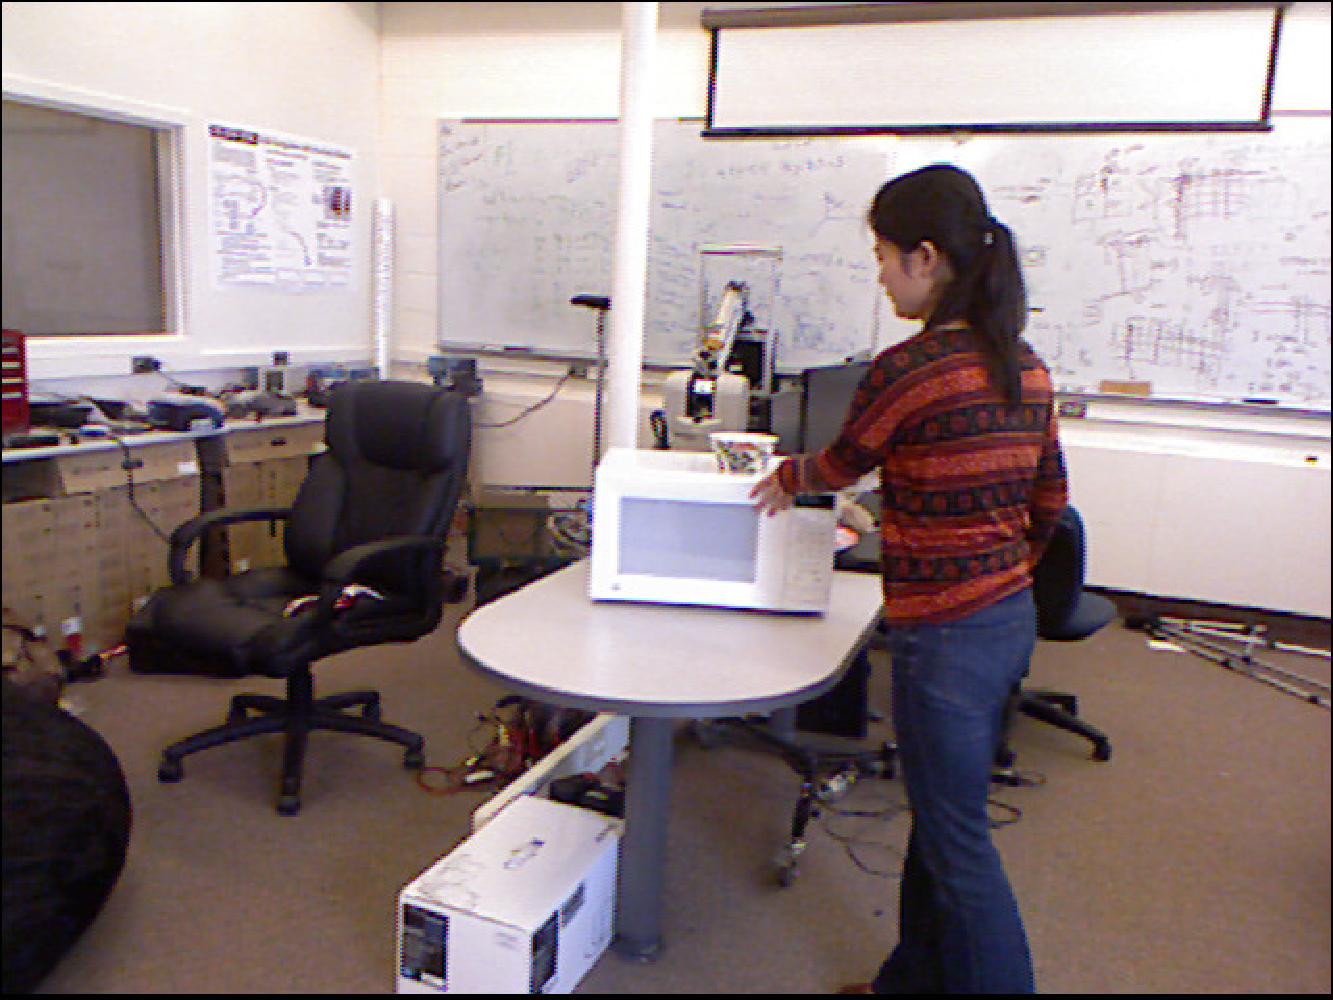
\includegraphics[width=0.225\textwidth]{f13}  \\ %\\%\begin{tabular}{p{3.6cm}p{3.6cm}p{3.6cm}p{3.6cm}}
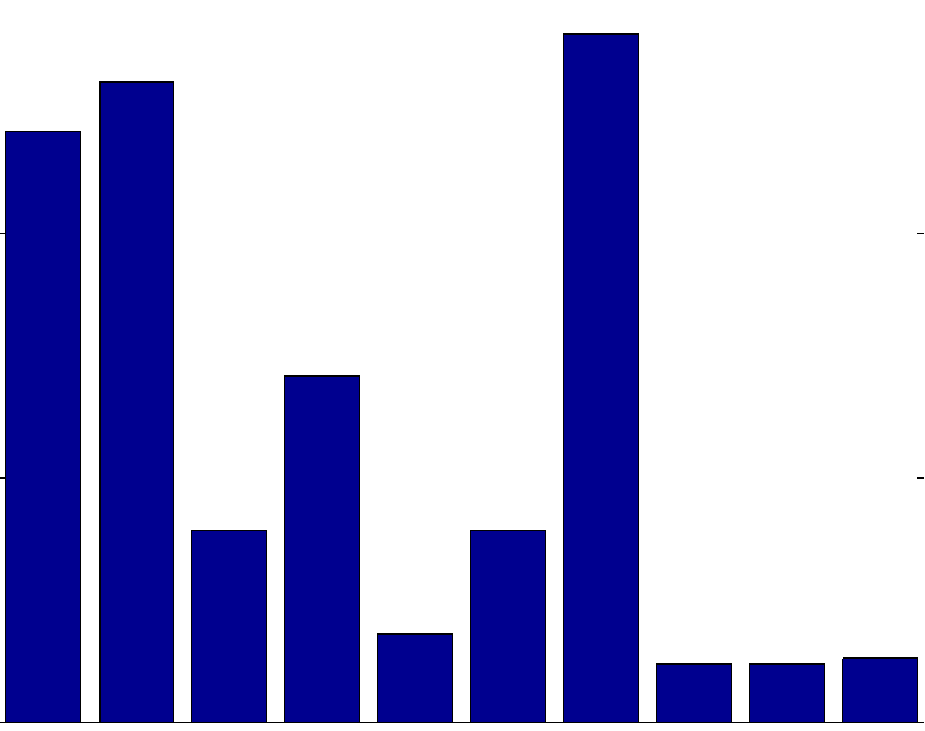
\includegraphics[width=0.225\textwidth, height=8mm]{P10} &
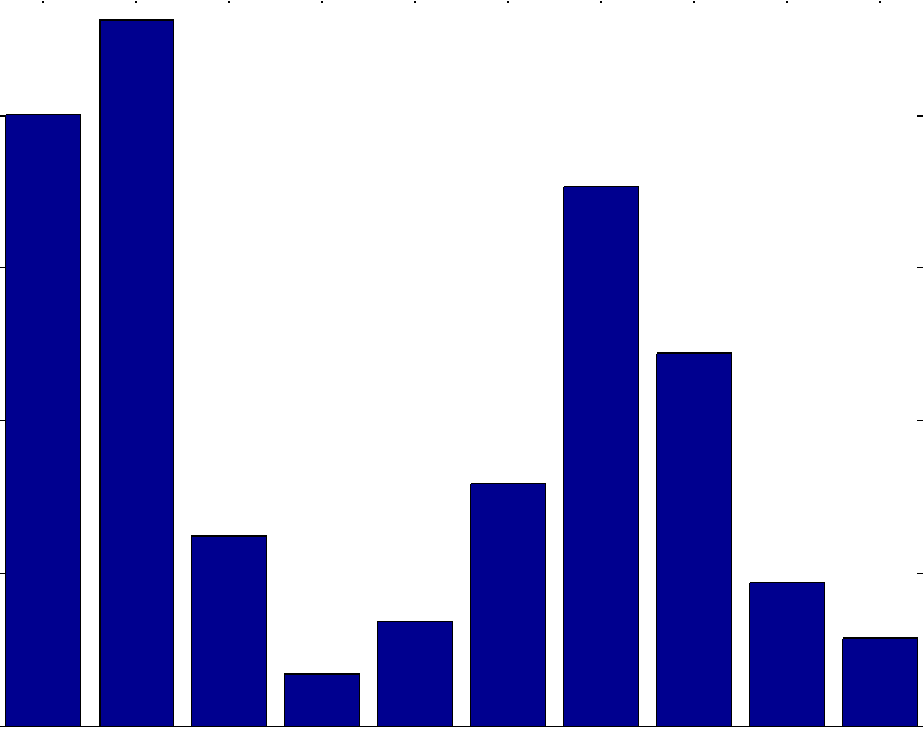
\includegraphics[width=0.225\textwidth, height=8mm]{P12P} &
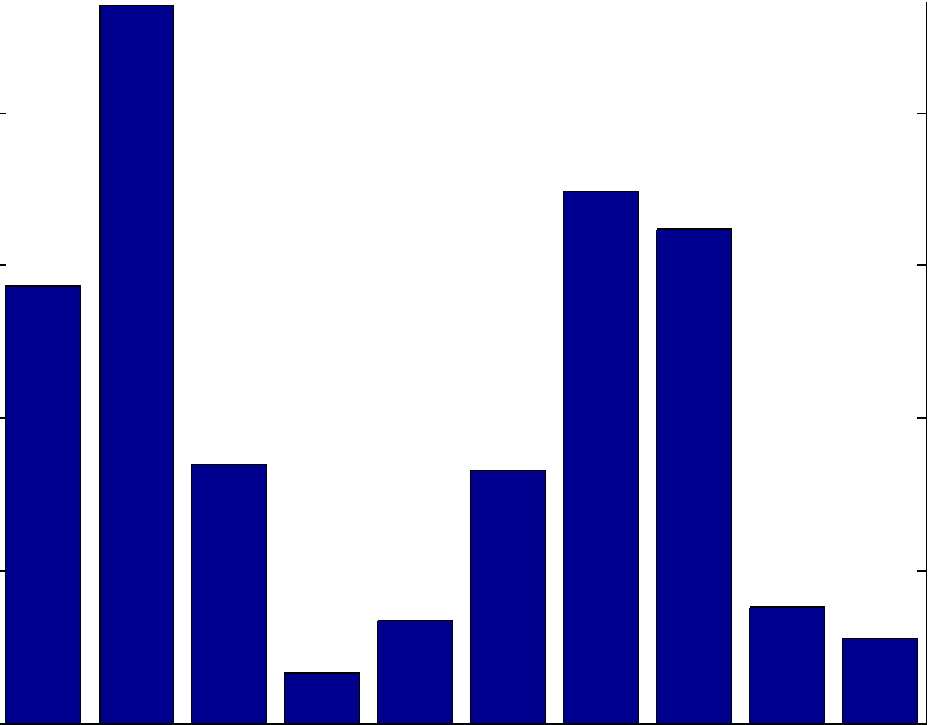
\includegraphics[width=0.225\textwidth, height=8mm]{P13P} &
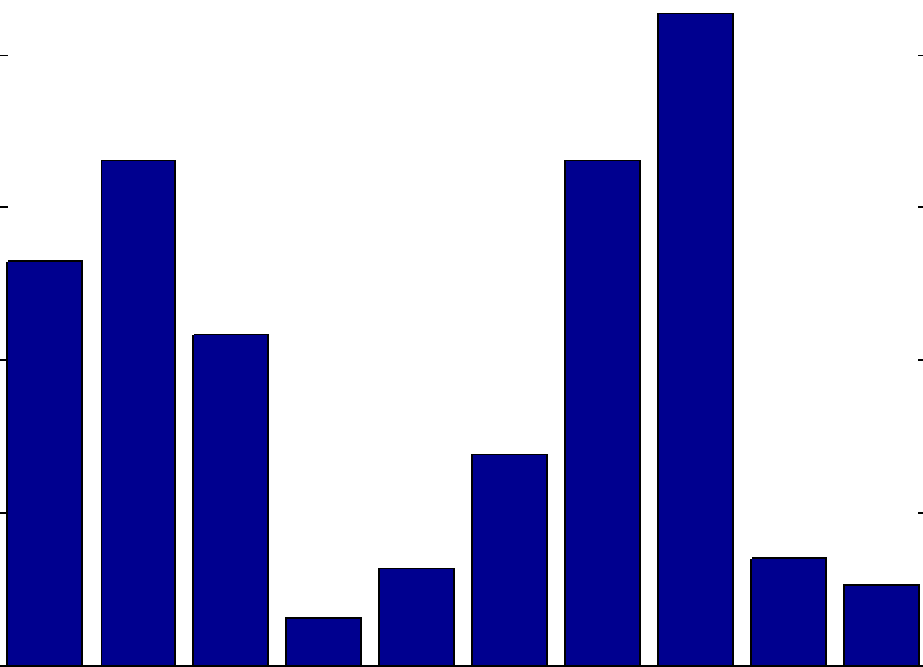
\includegraphics[width=0.225\textwidth, height=8mm]{P14P}  \\

\vspace{-6mm}\hspace{-1mm}\scalebox{0.84}{
\rotatebox[origin=r]{90}{reaching}\hspace{1mm}
\rotatebox[origin=r]{90}{moving}\hspace{1mm}
\rotatebox[origin=r]{90}{pouring}\hspace{1mm}
\rotatebox[origin=r]{90}{eating}\hspace{1mm}
\rotatebox[origin=r]{90}{drinking}\hspace{1mm}
\rotatebox[origin=r]{90}{opening}\hspace{1mm}
\rotatebox[origin=r]{90}{placing}\hspace{1mm}
\rotatebox[origin=r]{90}{closing}\hspace{1mm}
\rotatebox[origin=r]{90}{null}\hspace{1mm}
\rotatebox[origin=r]{90}{cleaning}}&
\vspace{-6mm}\hspace{-1mm}\scalebox{0.84}{
\rotatebox[origin=r]{90}{reaching}\hspace{1mm}
\rotatebox[origin=r]{90}{moving}\hspace{1mm}
\rotatebox[origin=r]{90}{pouring}\hspace{1mm}
\rotatebox[origin=r]{90}{eating}\hspace{1mm}
\rotatebox[origin=r]{90}{drinking}\hspace{1mm}
\rotatebox[origin=r]{90}{opening}\hspace{1mm}
\rotatebox[origin=r]{90}{placing}\hspace{1mm}
\rotatebox[origin=r]{90}{closing}\hspace{1mm}
\rotatebox[origin=r]{90}{null}\hspace{1mm}
\rotatebox[origin=r]{90}{cleaning}}&
\vspace{-6mm}\hspace{-1mm}\scalebox{0.84}{
\rotatebox[origin=r]{90}{reaching}\hspace{1mm}
\rotatebox[origin=r]{90}{moving}\hspace{1mm}
\rotatebox[origin=r]{90}{pouring}\hspace{1mm}
\rotatebox[origin=r]{90}{eating}\hspace{1mm}
\rotatebox[origin=r]{90}{drinking}\hspace{1mm}
\rotatebox[origin=r]{90}{opening}\hspace{1mm}
\rotatebox[origin=r]{90}{placing}\hspace{1mm}
\rotatebox[origin=r]{90}{closing}\hspace{1mm}
\rotatebox[origin=r]{90}{null}\hspace{1mm}
\rotatebox[origin=r]{90}{cleaning}}&
\vspace{-6mm}\hspace{-1mm}\scalebox{0.84}{
\rotatebox[origin=r]{90}{reaching}\hspace{1mm}
\rotatebox[origin=r]{90}{moving}\hspace{1mm}
\rotatebox[origin=r]{90}{pouring}\hspace{1mm}
\rotatebox[origin=r]{90}{eating}\hspace{1mm}
\rotatebox[origin=r]{90}{drinking}\hspace{1mm}
\rotatebox[origin=r]{90}{opening}\hspace{1mm}
\rotatebox[origin=r]{90}{placing}\hspace{1mm}
\rotatebox[origin=r]{90}{closing}\hspace{1mm}
\rotatebox[origin=r]{90}{null}\hspace{1mm}
\rotatebox[origin=r]{90}{cleaning}}
\end{tabular}
\end{tabular}

\begin{tabular}{p{5mm}@{}l}
\begin{tabular}{r}
\rotatebox[origin=r]{90}{\;\;\;\;\;\;\;Middle Frame}\\
\rotatebox[origin=l]{90}{Belief\;\;\;\;\;\;\;}
\end{tabular}
&
\begin{tabular}{p{3.7cm}p{3.7cm}p{3.7cm}p{3.7cm}}
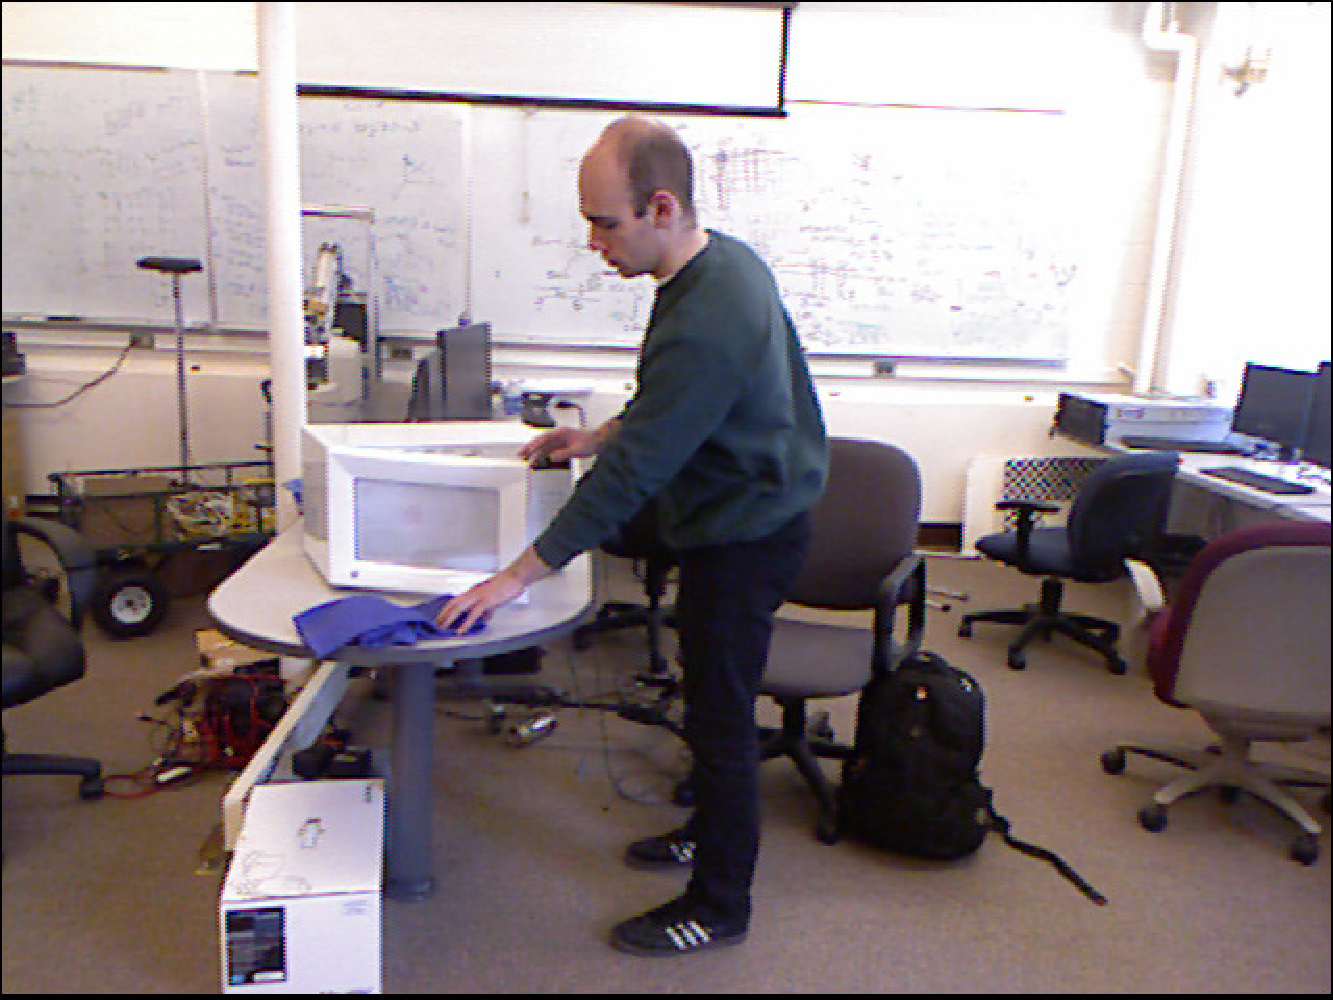
\includegraphics[width=0.225\textwidth]{l5} &
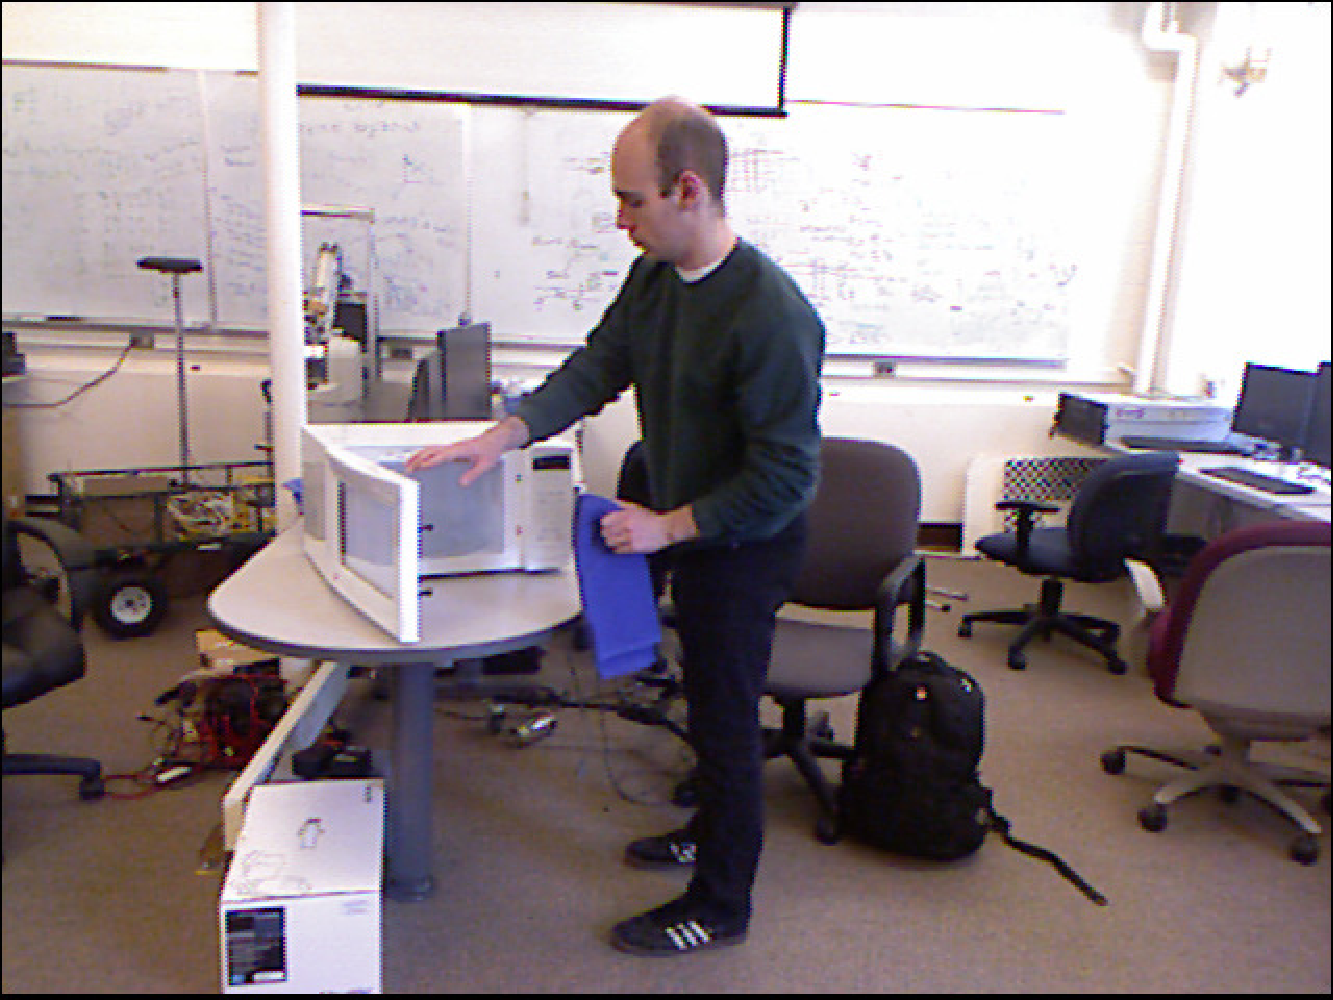
\includegraphics[width=0.225\textwidth]{l6} &
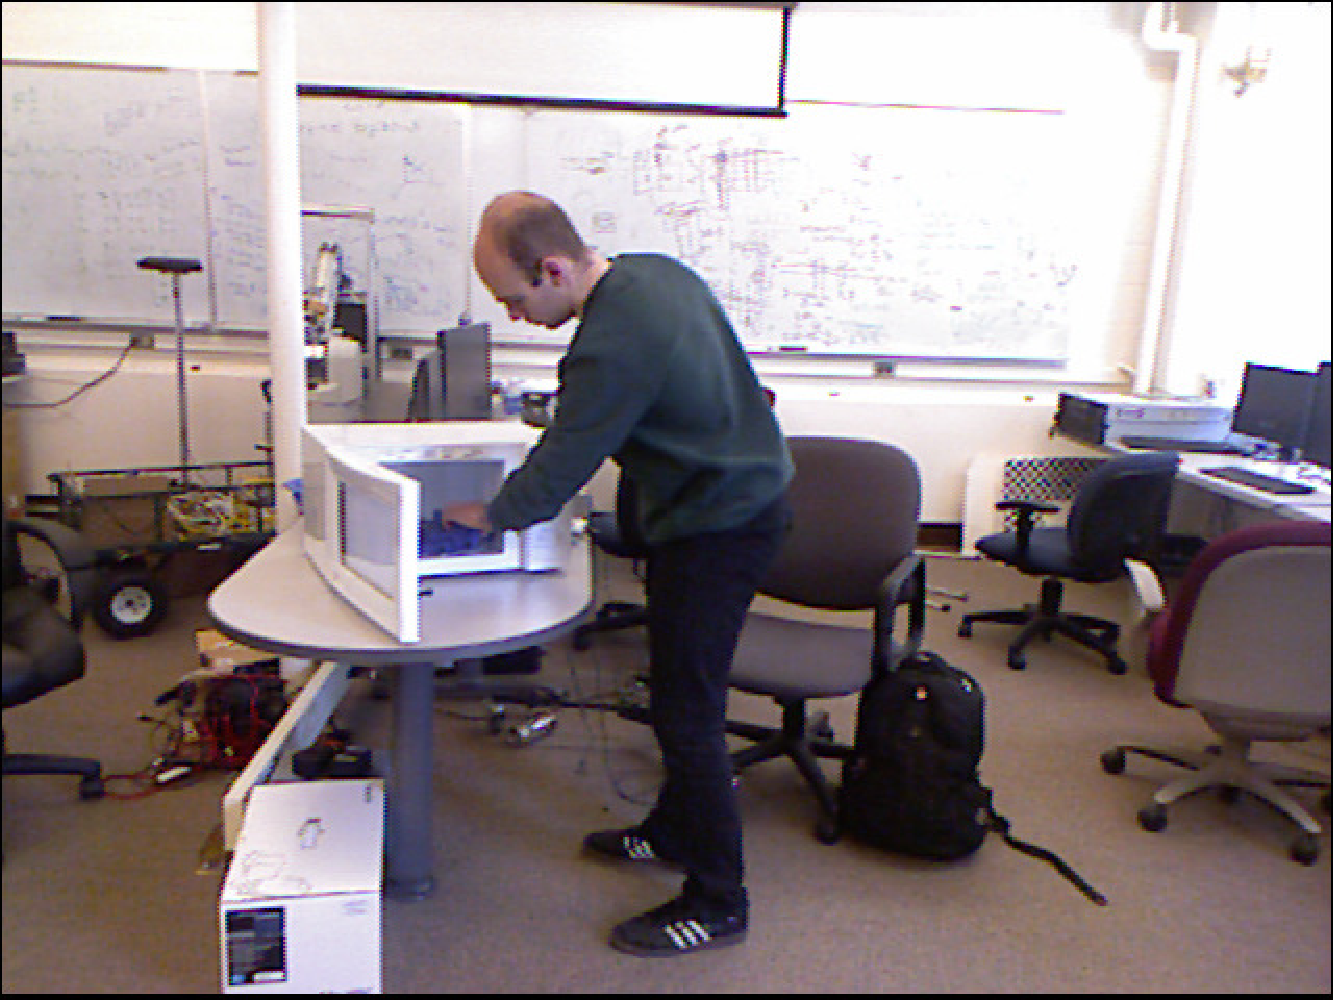
\includegraphics[width=0.225\textwidth]{l7} &
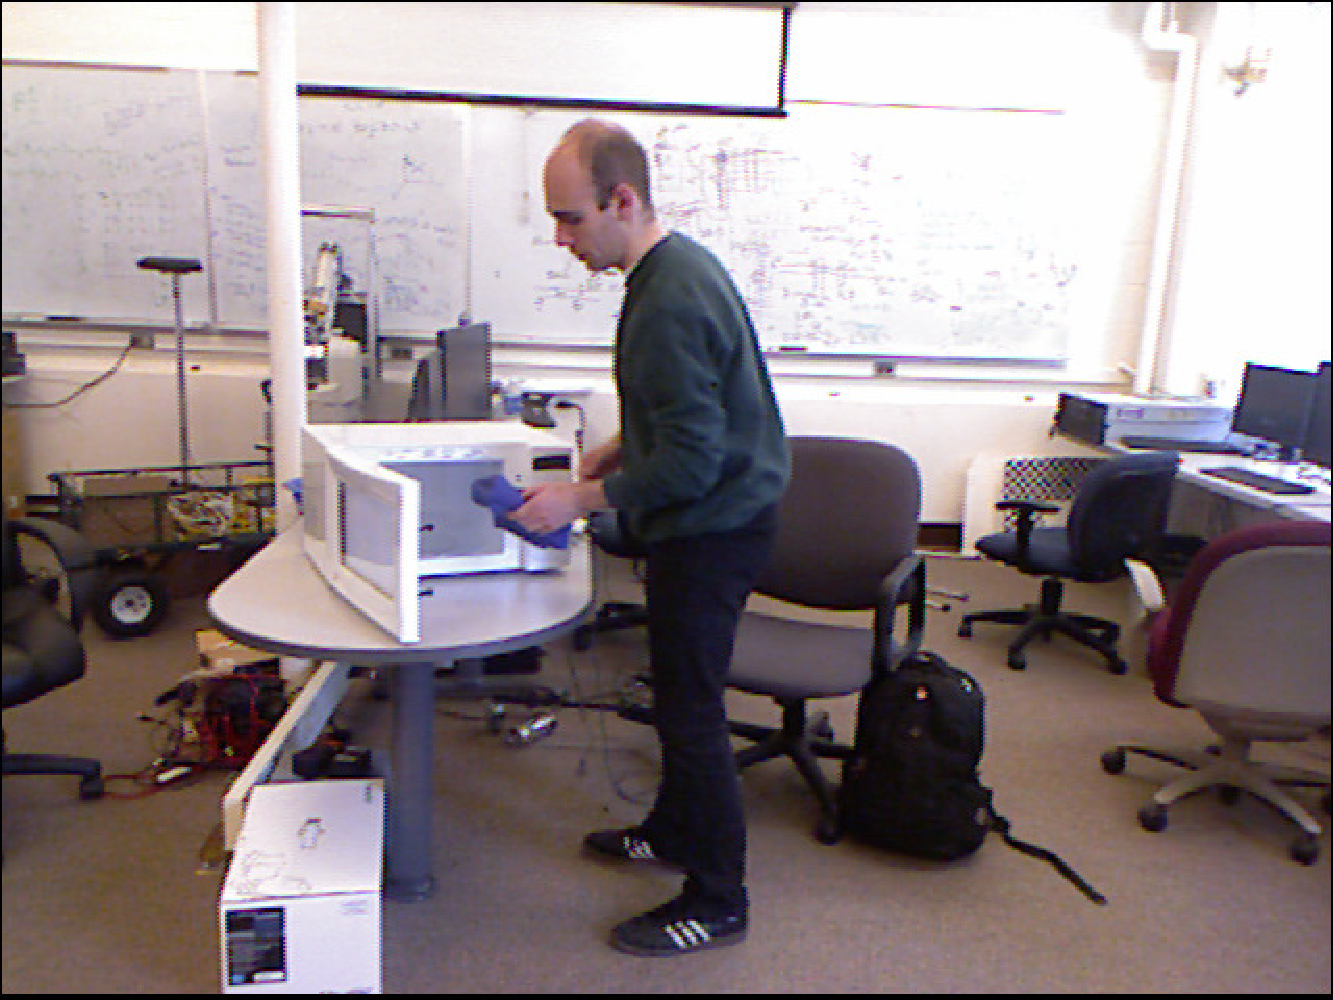
\includegraphics[width=0.225\textwidth]{l8}  \\
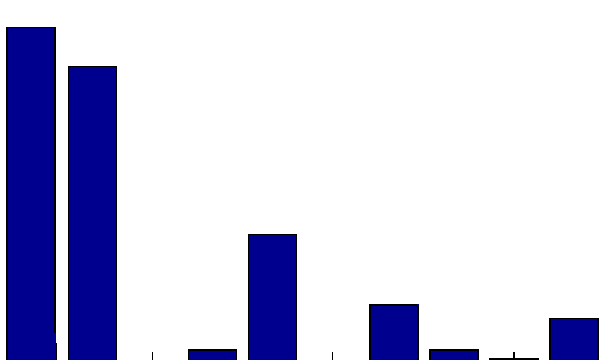
\includegraphics[width=0.225\textwidth, height=9mm]{bl5} &
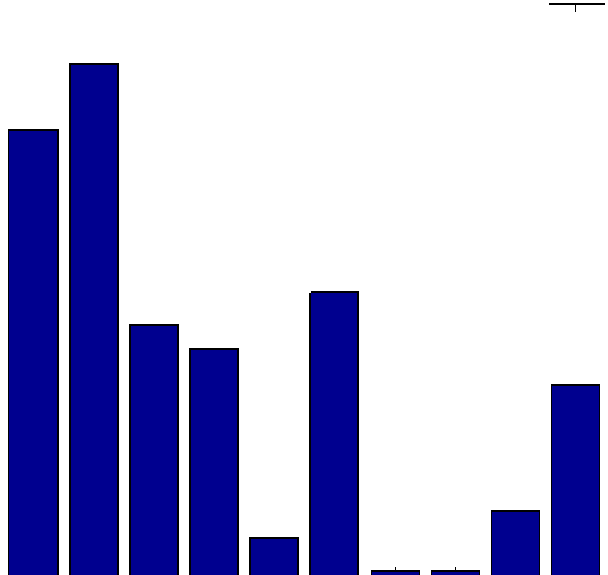
\includegraphics[width=0.225\textwidth, height=9mm]{bl6_2} &
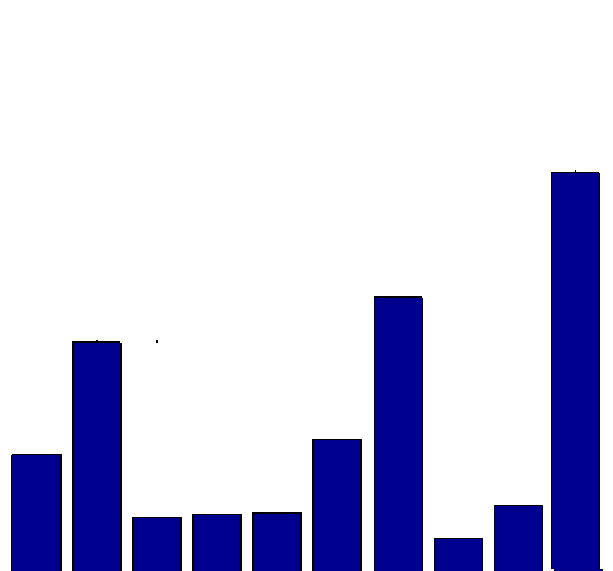
\includegraphics[width=0.225\textwidth, height=9mm]{bl7_2} &
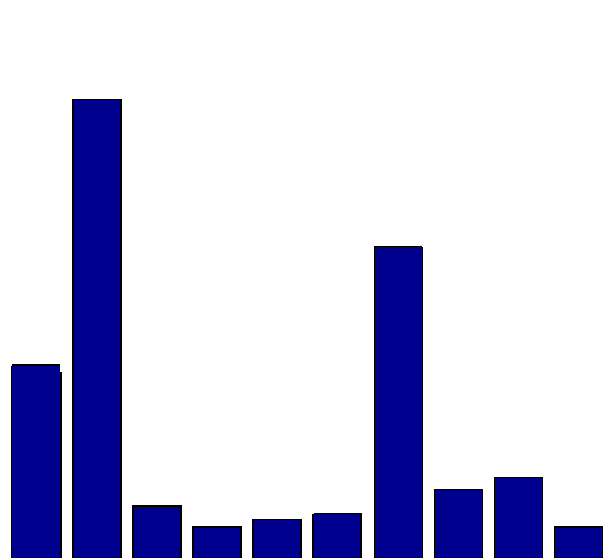
\includegraphics[width=0.225\textwidth, height=9mm]{bl8_2}  \\
\iffalse
\begin{tikzpicture}[remember picture,overlay]
\node[anchor=south west,inner sep=0] (image1)
  {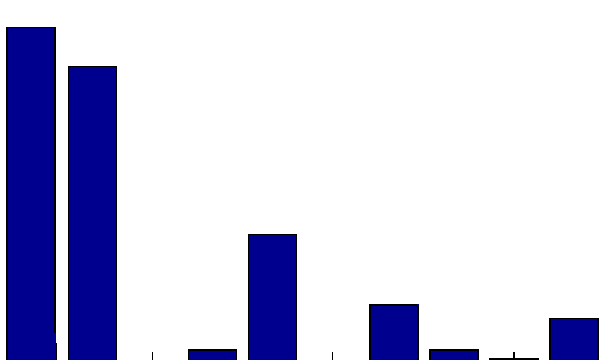
\includegraphics[width=0.22\textwidth, height=10mm]{bl5}};
\end{tikzpicture} &
\begin{tikzpicture}[remember picture,overlay]
\node[anchor=south west,inner sep=0] (image2)
  {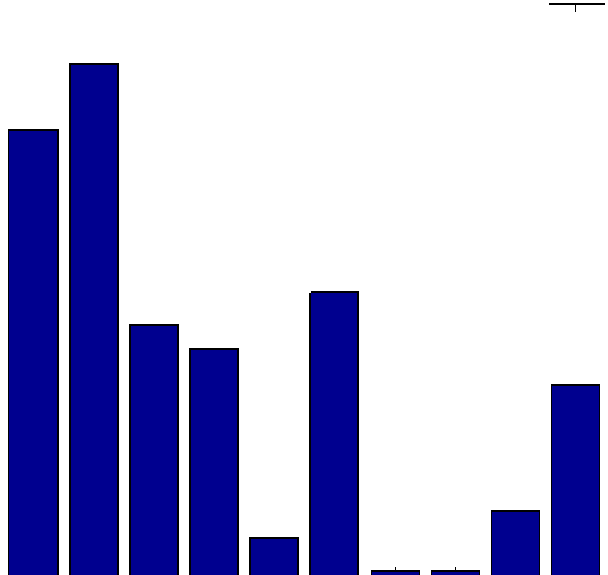
\includegraphics[width=0.22\textwidth, height=10mm]{bl6_2}};
\end{tikzpicture} &
\begin{tikzpicture}[remember picture,overlay]
\node[anchor=south west,inner sep=0] (image3)
  {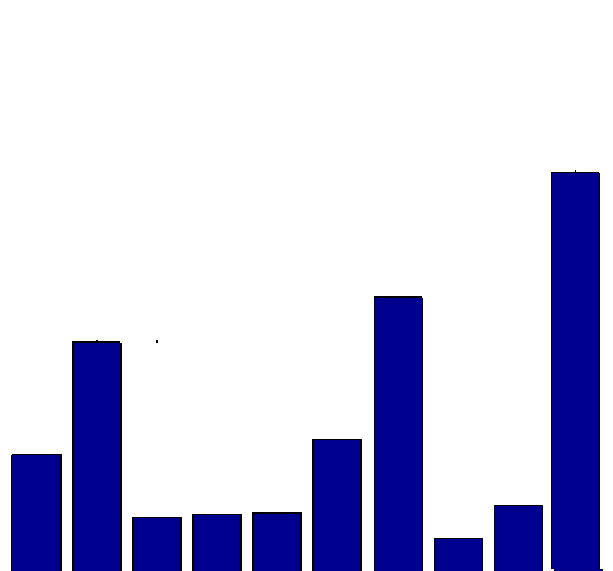
\includegraphics[width=0.22\textwidth, height=10mm]{bl7_2}};
\end{tikzpicture} &
\begin{tikzpicture}[remember picture,overlay]
\node[anchor=south west,inner sep=0] (image4)
  {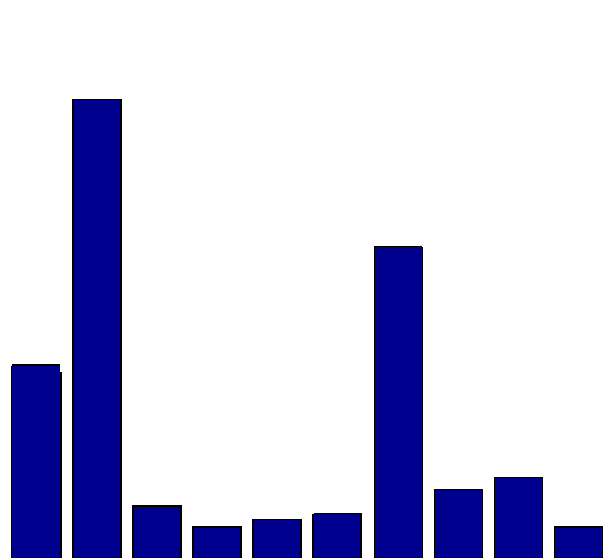
\includegraphics[width=0.22\textwidth, height=10mm]{bl8_2}};
\end{tikzpicture}
\begin{tikzpicture}[remember picture,overlay]
\draw[->,line width=2pt,red!80!black]
([yshift=-5pt,xshift=14pt]image4.west) |-
([yshift=-5pt,xshift=81pt]image3.west);
\draw[->,line width=2pt,red!80!black]
([yshift=0pt,xshift=81pt]image3.west) |-
([yshift=0pt,xshift=13pt]image2.west);
\draw[->,line width=2pt,red!80!black]
([yshift=-5pt,xshift=13pt]image2.west) |-
([yshift=-5pt,xshift=5pt]image1.west);
\end{tikzpicture}
\fi
\vspace{-6mm}\hspace{-1mm}\scalebox{0.84}{
\rotatebox[origin=r]{90}{reaching}\hspace{1mm}
\rotatebox[origin=r]{90}{moving}\hspace{1mm}
\rotatebox[origin=r]{90}{pouring}\hspace{1mm}
\rotatebox[origin=r]{90}{eating}\hspace{1mm}
\rotatebox[origin=r]{90}{drinking}\hspace{1mm}
\rotatebox[origin=r]{90}{opening}\hspace{1mm}
\rotatebox[origin=r]{90}{placing}\hspace{1mm}
\rotatebox[origin=r]{90}{closing}\hspace{1mm}
\rotatebox[origin=r]{90}{null}\hspace{1mm}
\rotatebox[origin=r]{90}{cleaning}}&
\vspace{-6mm}\hspace{-1mm}\scalebox{0.84}{
\rotatebox[origin=r]{90}{reaching}\hspace{1mm}
\rotatebox[origin=r]{90}{moving}\hspace{1mm}
\rotatebox[origin=r]{90}{pouring}\hspace{1mm}
\rotatebox[origin=r]{90}{eating}\hspace{1mm}
\rotatebox[origin=r]{90}{drinking}\hspace{1mm}
\rotatebox[origin=r]{90}{opening}\hspace{1mm}
\rotatebox[origin=r]{90}{placing}\hspace{1mm}
\rotatebox[origin=r]{90}{closing}\hspace{1mm}
\rotatebox[origin=r]{90}{null}\hspace{1mm}
\rotatebox[origin=r]{90}{cleaning}}&
\vspace{-6mm}\hspace{-1mm}\scalebox{0.84}{
\rotatebox[origin=r]{90}{reaching}\hspace{1mm}
\rotatebox[origin=r]{90}{moving}\hspace{1mm}
\rotatebox[origin=r]{90}{pouring}\hspace{1mm}
\rotatebox[origin=r]{90}{eating}\hspace{1mm}
\rotatebox[origin=r]{90}{drinking}\hspace{1mm}
\rotatebox[origin=r]{90}{opening}\hspace{1mm}
\rotatebox[origin=r]{90}{placing}\hspace{1mm}
\rotatebox[origin=r]{90}{closing}\hspace{1mm}
\rotatebox[origin=r]{90}{null}\hspace{1mm}
\rotatebox[origin=r]{90}{cleaning}}&
\vspace{-6mm}\hspace{-1mm}\scalebox{0.84}{
\rotatebox[origin=r]{90}{reaching}\hspace{1mm}
\rotatebox[origin=r]{90}{moving}\hspace{1mm}
\rotatebox[origin=r]{90}{pouring}\hspace{1mm}
\rotatebox[origin=r]{90}{eating}\hspace{1mm}
\rotatebox[origin=r]{90}{drinking}\hspace{1mm}
\rotatebox[origin=r]{90}{opening}\hspace{1mm}
\rotatebox[origin=r]{90}{placing}\hspace{1mm}
\rotatebox[origin=r]{90}{closing}\hspace{1mm}
\rotatebox[origin=r]{90}{null}\hspace{1mm}
\rotatebox[origin=r]{90}{cleaning}}
\end{tabular}
\end{tabular}
\caption{\textbf{Anticipated belief over activity.} In the first and third row, we show a middle frame of the temporal segment. In the second and fourth row, we show the anticipated belief we computed for the middle frame. Note that frames are not visible to the algorithm and only included for evaluation.}
%\vspace{-4mm}
\label{abcd}
%\end{singlespace}
\end{figure}


\noindent {\bf Data:} We use CAD-120 \cite{hemaIJRR} dataset in order to evaluate our method. CAD-120 dataset includes 120 RGB-D videos of four different subject performing activities \emph{reaching, moving, pouring, etc.} while interacting with objects having affordances \emph{reachable, movable, pourable, etc.}. There are 10 activity classes and 12 object affordance classes.

\noindent {\bf Experimental Setup:} For computing the features and learning the CRF parameters, we follow the approach and the code in \cite{hemaIJRR}. Following the convention in \cite{hemaIJRR}, we use 4-fold cross-validation by training over the data from 3 subjects and testing on the remaining subject. We then average the results over 4-folds. We implemented the rCRF as we explain in Algorithm~\ref{alg:recursive} with the following parameters obtainded via cross-validation; we sampled $M=15$ diverse samples and ran the recursive message updates with the number of iterations limit as $5$.

For the anticipation setting, In order to experiment the $\tau$ seconds into the future anticipation, we experiment over all feasible anticipation scenarios. In other words, we anticipated the time instant $t+\tau$ by using the segments $1\ldots t$ for all $t<T-\tau$, where $T$ is the length of the video. Then, we averaged the score over all feasible experiments.

\noindent {\bf Baseline Algorithms:} In detection setting, we compare the detection results of the rCRF to MAP solution of the spatiotemporal CRF in \cite{hemaIJRR}. We also included the state-of-the art activity detection results from Hu et al. \cite{latentIcra}. Moreover, \cite{latentIcra} is not based on object affordances and it only outputs activity detections. For the anticipation, we compare the rCRF with the state-of-the-art anticipation methods ATCRF \cite{hemaAnt} and GP-LCRF\cite{gpcrf}. We also include DCRF\cite{ddcrf}. In order to evaluate the contribution of the recursive modeling and the structured diversity separately, we also compare the rCRF with a recursive approach without diversity and a diversity-based approach without recursive modeling baselines.

The DivMBest algorithm in \cite{divmbest} uses the diverse sampling method to sample CRFs defined over each frame separately. DivMBest\cite{divmbest} then finds the most likely sequence via Viterbi algorithm. Since it is missing the recursive modeling, it serves as \emph{structured diversity without recursive filtering} baseline. We replace the diversity-based sampling in our method with Gibbs sampler and consider it as \emph{recursive filtering approach without structured diversity} baseline. For the Gibbs sampling, we sampled $50$ samples per temporal segment. We denote the recursive approach with Gibbs sampling as \emph{\mbox{"rCRF w/o div"}} while tabulating the results.

\noindent {\bf Evaluation Metrics:} For activity detection, we compute the ratio of the correctly classified labels (\emph{micro precision}) and the averages of the precision and recall values computed for each activity and object affordance classes (\emph{macro precision} and \emph{macro recall}). For anticipation, we record the ratio of the correctly classified labels \emph{micro precision}, the average of the f-1 score that is computed for each activity and object affordance class (\emph{macro f-1 score}), and the precision of the top 3 anticipated labels (\emph{robot anticipation metric}). While computing the \emph{robot anticipation metric}; if any of the top 3 anticipation is correct, it is counted as true positive.

\noindent {\bf Accuracy of the rCRF in detection setting.}
We evaluate the rCRF for activity detection and summarize the results in Table~\ref{Tdet}. Table~\ref{Tdet} suggests that the rCRF outperforms the MAP solution \cite{hemaIJRR} and performs similarly with the state-of-the-art solution \cite{latentIcra}. Since rCRF and \cite{hemaIJRR} are using the same spatial relations, the performance difference is due to the modeling of the temporal relations in rCRF. We use \mbox{first-order} statistics as temporal dynamics, and they are quite accurate as shown in the heatmap in Figure~\ref{heatmap}. They also capture semantic information like objects become stationary after being used.

\begin{figure}
  \subfigure[Human Activity]{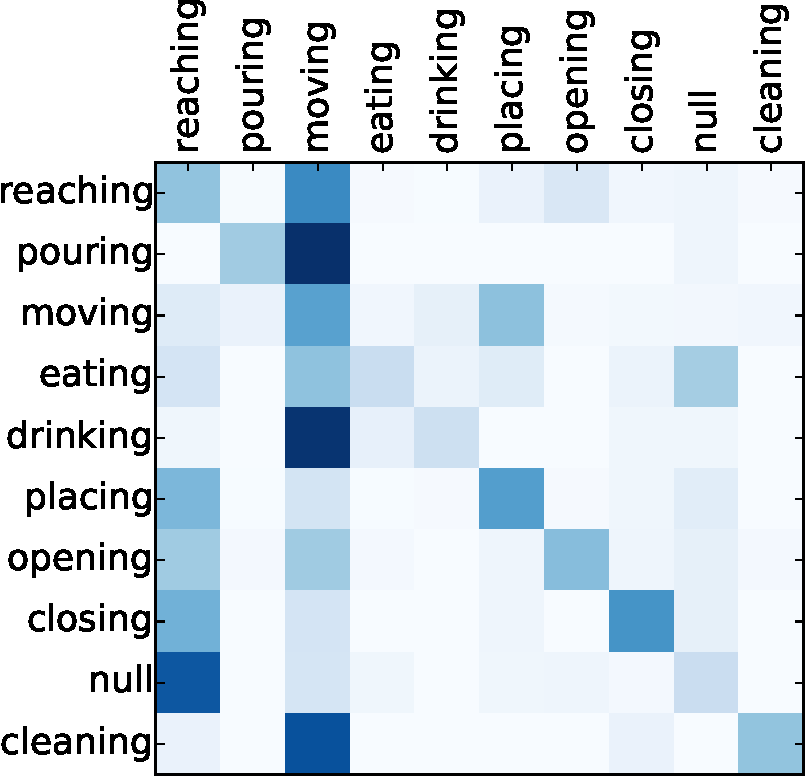
\includegraphics[width=0.48\textwidth]{tranAct}}~
  \subfigure[Object Affordance]{ 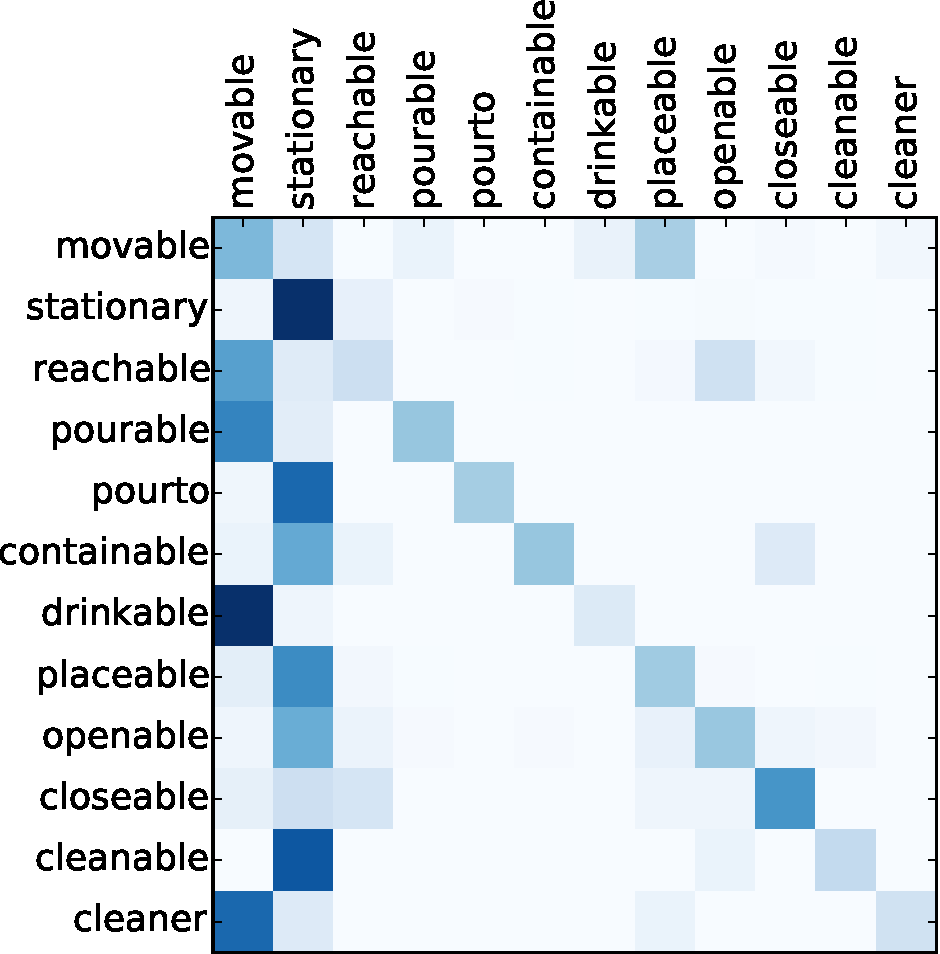
\includegraphics[width=0.48\textwidth]{tranObj}}
  \caption{Heatmap of the first-order statistics of activity and object affordance classes. They are used as temporal dynamics by rCRF.}
  \label{heatmap}
\end{figure}

\noindent {\bf Accuracy of the rCRF in anticipation setting.}
We evaluate the accuracy of the belief we compute via rCRF, both quantitatively and qualitatively. For qualitative evaluation, we show the segment that we are anticipating the belief over, as well as the belief we obtain in Figure~\ref{abcd}. Please note that, this visual information is not visible to the algorithm, and it is only included for the subjective evaluation.

As shown in the figure, anticipated belief is capturing the scene accurately. Belief is accurate even for the case of concurrent activities. For example, in the second column of the second row in Figure \ref{abcd}, subject is reaching the microwave and moving the cleaner. Our method assigns similar likelihood values to both reaching and moving.

We also perform quantitative analysis over anticipation accuracy. We anticipate 3 seconds into the future and summarize the results in Table~\ref{Tant}. As shown in the Table~\ref{Tant}, rCRF outperforms the state-of-the-art heuristic method \cite{hemaAnt} and the GP-LCRF method \cite{gpcrf} significantly as well as all other baselines. We believe this result is due to the accurate joint-modeling of the temporal relations and the CRF model. We further analysed this behaviour in the subsequent sections.

\begin{table}[ht]
\centering
\tabcolsep=0.7mm
\footnotesize
%\vspace{-1mm}
\caption{\textbf{Detection Performance over CAD-120.}  We compare rCRF with MAP solution and baselines for detections accuracy.}
%\vspace{-1mm}
\begin{tabular}{@{}l@{}|ccc|ccc@{}} \hline
& \multicolumn{3}{@{}|c@{}}{Sub-activity } &   \multicolumn{3}{@{}|c@{}}{Object Affordance } \\ \hline
& micro & \multicolumn{2}{@{}c|@{}}{macro} &   micro & \multicolumn{2}{@{}c@{}}{macro} \\
% \hline
 & prec(\%) & prec(\%) & rec(\%) &   prec(\%) & prec(\%) & rec(\%) \\
\hline
Chance & $10.0${\scriptsize $\pm 0.1$}  & $10.0${\scriptsize $\pm 0.1$}  & $10.0${\scriptsize $\pm 0.1$}  & $8.3${\scriptsize $\pm 0.1$}  & $8.3${\scriptsize $\pm 0.1$}  & $8.3${\scriptsize $\pm 0.1$}  \\
Hu et al.\cite{latentIcra} & $67.8${\scriptsize $\pm 1.4$}  &  $65.5${\scriptsize $\pm 3.5$}&  $\mathbf{63.5}${\scriptsize $\mathbf{\pm 6.6}$}  & N/A & N/A & N/A \\
MAP Sol\cite{hemaIJRR} & $63.4${\scriptsize $\pm 1.6$}  &  $65.3${\scriptsize $\pm 2.3$}&  $54.0${\scriptsize $\pm 4.6$}  & $79.4${\scriptsize $\pm 0.8$} & $62.5${\scriptsize $\pm 5.4$} & $50.2${\scriptsize $\pm 4.9$} \\
DivMBest\cite{divmbest}& $64.0${\scriptsize $\pm 1.3$} & $61.7${\scriptsize $\pm 2.1$} & $56.4${\scriptsize $\pm 2.7$} & $80.1${\scriptsize $\pm 1.0$} & $76.2${\scriptsize $\pm 2.5$} & $53.2${\scriptsize $\pm 3.2$} \\
DCRF\cite{ddcrf}& $61.2${\scriptsize $\pm 2.1$} & $62.8${\scriptsize $\pm 2.8$} & $54.3${\scriptsize $\pm 1.5$} & $71.9${\scriptsize $\pm 2.9$} & $80.6${\scriptsize $\pm 2.4$} & $62.5${\scriptsize $\pm 3.6$} \\
rCRF w/o div& $61.2${\scriptsize $\pm 1.8$} & $64.0${\scriptsize $\pm 1.8$} & $52.7${\scriptsize $\pm 3.8$} & $75.2${\scriptsize $\pm 2.4$} & $79.3${\scriptsize $\pm 3.1$} & $63.7${\scriptsize $\pm 2.9$} \\
rCRF&  $\mathbf{68.1}${\scriptsize$\mathbf{\pm 1.3}$} & $\mathbf{66.1}${\scriptsize $\mathbf{\pm 2.7}$} & $57.2${\scriptsize $\pm 3.9$} & $\mathbf{81.5}${\scriptsize $\mathbf{\pm 1.1}$} & $\mathbf{85.2}${\scriptsize $\mathbf{\pm 2.4}$} & $\mathbf{71.6}${\scriptsize $\mathbf{\pm 3.9}$} \\
\hline
\end{tabular}
%\end{singlespace}
\label{Tdet}
\end{table}
\begin{table}[ht]
\centering
\tabcolsep=0.7mm
\footnotesize
\vspace{-1mm}
\caption{\textbf{Anticipation performance for the anticipating 3 seconds in the future.} We compare rCRF with state-of-the-art anticipation algorithm and baselines for anticipation accuracy.}
\vspace{-1mm}
\begin{tabular}{@{}l@{}|ccc|ccc@{}} \hline
& \multicolumn{3}{@{}|c@{}}{Sub-activity } &   \multicolumn{3}{@{}|c@{}}{Object Affordance } \\ \hline
& micro & macro & robot ant. &  micro & macro & robot ant.   \\
Method & prec(\%) & f1-scr(\%) & metric(\%) & prec(\%) & f1-scr(\%) & metric(\%) \\ \hline
Chance & $10.0${\scriptsize $\pm 0.1$} & $10.0${\scriptsize $\pm 0.1$}  & $30.0${\scriptsize $\pm 0.1$} & $8.3${\scriptsize $\pm 0.1$} & $8.3${\scriptsize $\pm 0.1$}  & $24.9${\scriptsize $\pm 0.1$}  \\
GP-LCRF \cite{gpcrf} & $52.1${\scriptsize $\pm 1.2$} & $43.2${\scriptsize $\pm 1.5$} &  $76.1${\scriptsize $\pm 1.5$}  & $68.1${\scriptsize$\pm 1.0$}  & $44.2${\scriptsize $\pm 1.2$}  & $74.9${\scriptsize $\pm 1.1$}  \\
ATCRF \cite{hemaAnt} & $47.7${\scriptsize $\pm 1.6$} & $37.9${\scriptsize $\pm 2.6$} &  $69.2${\scriptsize $\pm 2.1$}  & $66.1${\scriptsize $\pm 1.9$}  & $36.7 ${\scriptsize $\pm 2.3$}  & $71.3${\scriptsize $\pm 1.7$}  \\
DivMBest\cite{divmbest}& $47.9${\scriptsize $\pm 1.4$} & $43.2${\scriptsize $\pm 3.6$} & $71.5${\scriptsize $\pm 2.7$} & $61.3${\scriptsize $\pm 1.4$} & $56.3 ${\scriptsize $\pm 2.1$} & $73.3${\scriptsize $\pm 0.5$} \\
DCRF\cite{ddcrf}& $48.3${\scriptsize $\pm 2.6$} & $35.4${\scriptsize $\pm 1.8$} & $66.6${\scriptsize $\pm 1.1$} &
$55.2${\scriptsize $\pm 3.1$} & $48.5${\scriptsize $\pm 3.1$} & $71.24${\scriptsize $\pm 2.2$} \\
rCRF w/o div& $49.6${\scriptsize $\pm 2.1$} & $39.7${\scriptsize $\pm 2.6$} & $65.1${\scriptsize $\pm 1.1$} & $56.2${\scriptsize $\pm 1.9$} & $47.4${\scriptsize $\pm 3.1$} & $70.8${\scriptsize $\pm 2.5$} \\
rCRF & $\mathbf{54.3}${\scriptsize $\mathbf{\pm 3.9}$} & $\mathbf{45.8}${\scriptsize $\mathbf{\pm 2.7}$} & $\mathbf{76.5}${\scriptsize $\mathbf{\pm 2.6 }$}  & $\mathbf{78.7}${\scriptsize $\mathbf{\pm 3.4}$} &$\mathbf{74.9}${\scriptsize $\mathbf{\pm 3.8}$} & $\mathbf{82.1}${\scriptsize $\mathbf{\pm 2.9}$} \\
\hline
\end{tabular}
\label{Tant}
\end{table}

\noindent {\bf How important is the recursive modeling?}
DivMBest\cite{divmbest} is the application of the structured diversity without recursive modeling of the Bayesian filtering. In all experiments (Table~\ref{Tdet} and \ref{Tant}), rCRF outperforms the DivMBest \cite{divmbest}. We believe this is because rCRF samples  $p(y^t|x^1,\ldots,x^T)$ instead of $p(y^t|x^t)$ as in the case of \cite{divmbest}. In other words, DivMBest \cite{divmbest} samples without considering temporal relations; on the contrary, we sample the full belief directly.

Moreover, the improvement over the DCRF model shows the important of accurate recursive modeling. DCRF uses the recursive modeling without the proposed conversion of the discrimantive likelihood into generative one and it performs poorly. Hence, the proposed conversion is a necessary step.

We also studied the effect of anticipation horizon. We computed precision of all methods for horizons between 1 and 10 seconds and plotted in Figure~\ref{antHor} and \ref{objHor}. We see significant improvements over longer anticipation time horizons.%\footnote{Since ATCRF \cite{hemaAnt} and GP-LCRF \cite{gpcrf} are using the same method to anticipate the future activities and they only differ in modeling details of humans, they behave similarly versus anticipation time as shown in \cite{gpcrf} and we only included \cite{hemaAnt} in the plot.}
%  and we only included \cite{hemaAnt} in the plot for the sake of clarity.
%We only show the result on object affordance anticipation and rest of the results are included in the supplementary material.

In Figure~\ref{antHor} and \ref{objHor}, accuracy of all algorithms decreases with the increasing horizon. One interesting observation is decrease rate of DivMBest is steeper than others. Since DivMBest misses the recursive nature of the problem, accuracy of the belief it computes is limited; hence, the resulting belief does not stay informative with increasing horizon.

\begin{figure}[ht]
\begin{center}
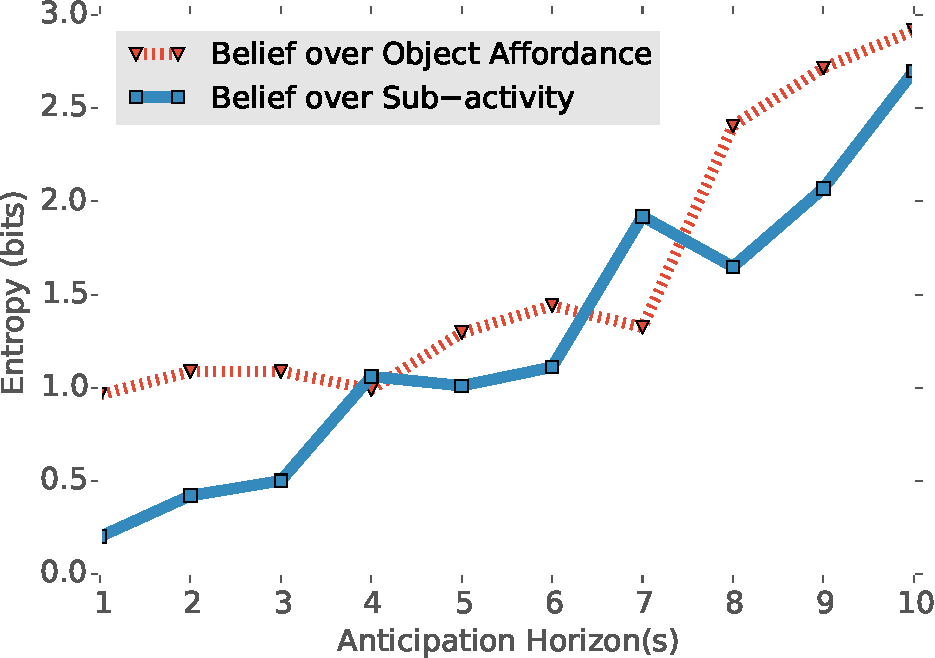
\includegraphics[width=\textwidth]{entTwo}
\caption{Entropy of the belief vs. time \emph{(uniform dist. has $\approx 3.32$ bit entropy)}}
\label{entRop}
\end{center}
\end{figure}

We further computed the entropy of the belief rCRF computes and plotted its average in Figure~\ref{entRop}. The decrease rate of the accuracy is much smaller than the increase rate of the entropy. In summary, recursive modeling is necessary for an accurate belief estimation and rCRF computes flatter yet still informative beliefs with increasing horizon.

\noindent {\bf How to efficiently cover the output space?}
In order to see the effect of structural diversity on covering the output space, we compare the rCRF with a version of it in which we replace diverse sampling with the Gibbs sampler. As expected, Gibbs sampler only sampled the small region around the posterior and failed to cover the output space. Within all experiments, rCRF outperforms Gibbs sampler baseline. Another interesting observation is, as shown in Figure~\ref{antHor}\&\ref{objHor}, although Gibbs sampler based method performed slightly better than other baselines for short horizon activity anticipation, it performed much worse for object affordance. We believe this is because of the dimensionality. Activity space has dimension $10^{T}$ whereas the object affordance space has dimension $12^{T\cdot M}$ where $T$ is the length of the video and $M$ is the number of objects. Hence, diversity plays bigger role with increasing dimension. Moreover, \cite{hemaAnt} uses the domain knowledge by selectively sampling points around the hand, etc. and it performs better than both baselines with increasing horizon. We believe this result is due to the efficient coverage of the output space with heuristics.

\begin{figure}[t]
  \centering
  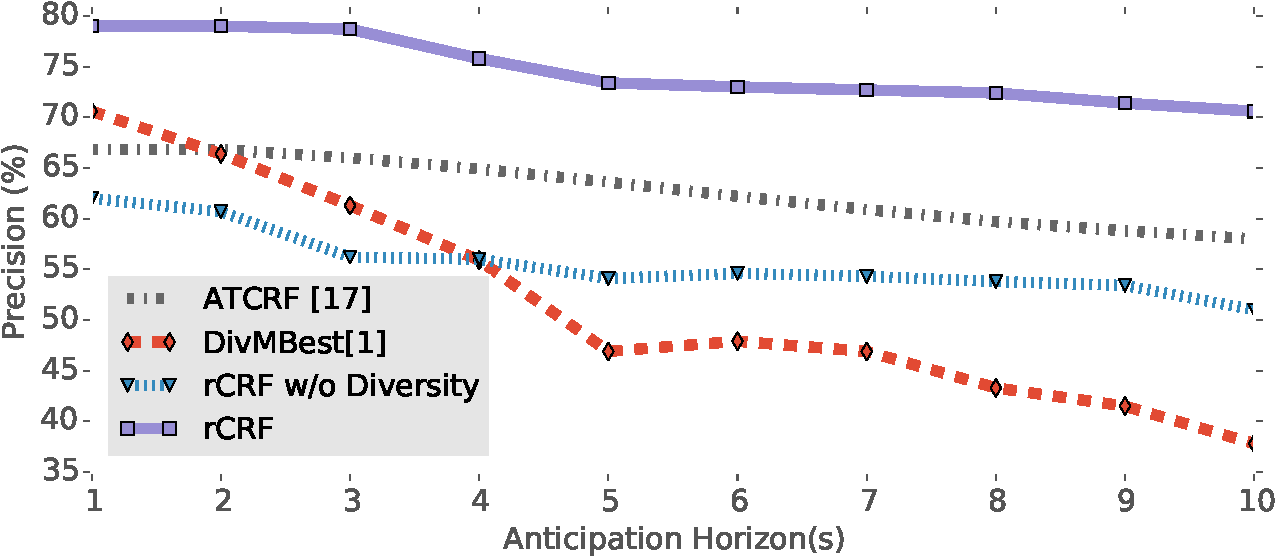
\includegraphics[width= \textwidth]{AntO}
\caption{Precision vs. anticipation horizon for object affordance.}
\label{antHor}
\end{figure}

\begin{figure}[h!]
  \centering
  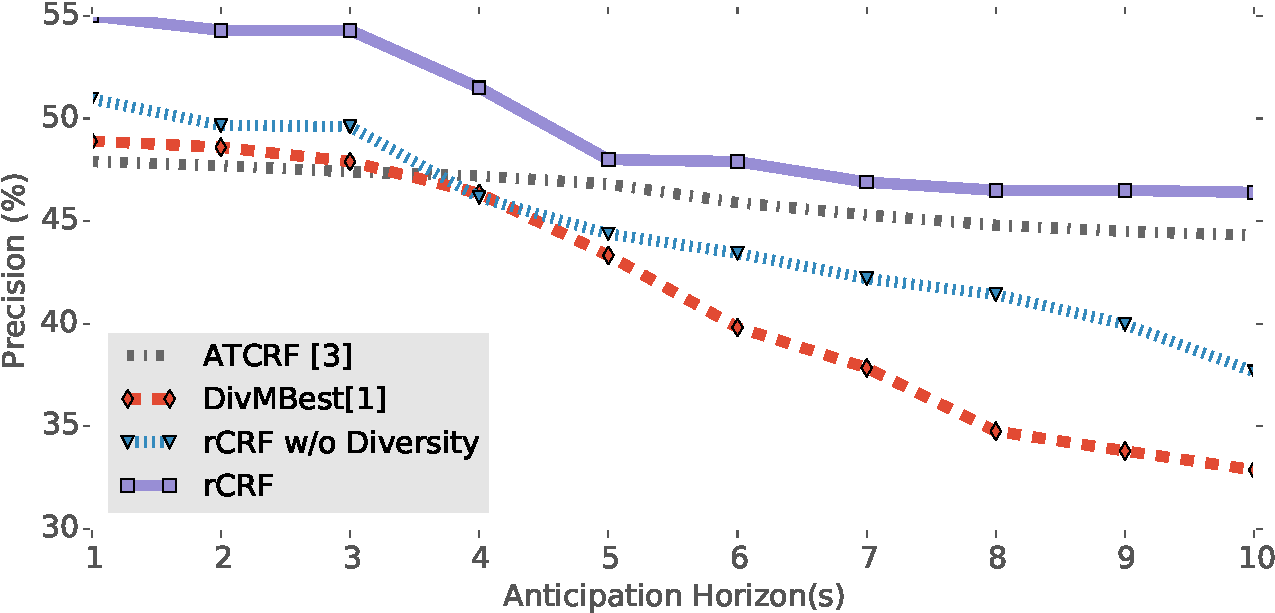
\includegraphics[width=\textwidth]{AntA}
\caption{Precision vs. anticipation horizon for subject activities.}
\label{objHor}
\end{figure}

\noindent {\bf Computationally-efficient inference:}
We evaluated the computational efficiency by computing the average computation time for anticipating 3 second in the future via rCRF and the fastest available anticipation algorithm (the ATCRF\cite{hemaAnt}). Within our experiments, we did not include any pre-processing or feature extraction computation (they are same for all algorithms). Our experiments suggest that the rCRF is faster than \cite{hemaAnt} as shown in Table~\ref{speed}. Hence, rCRF model outperforms the state-of-the-art anticipation algorithm in terms of speed in addition to the accuracy.
\begin{table}[h!]
  \centering
%  \vspace{-2mm}
\caption{Computation time for anticipating 3 seconds in the future excluding pre-processing (\emph{see supplementary material for details}).}
%\vspace{-2mm}
  \begin{tabular}{|cc|cc|}
    \hline
  ATCRF \cite{hemaAnt} \; \; & \; \; 34.1s  \; \;  \; & \; \; \;  rCRF \; \; & \; \;  1.41s \\ \hline
  \end{tabular}
  \vspace{-1mm}
  \label{speed}
\end{table}
%\vspace{-2mm}

\noindent {\bf Can rCRF generalize to RGB data?:}
Since there is no RGB activity dataset with object labels, it is hard to compare our algorithm in the RGB activity analysis setting. Removing the concept of the objet form the graph, makes it a chain-CRF and the inference and learning becomes straightforward. However, we still implement our rCRF over a linear-chain CRF for RGB activity analysis. We based our implementation on MPII cooking activity dataset \cite{mpi_cooking} and use the publicly distributed features from the authors webpage. The shared features are HOG, HOF, dense trajetory features and  MBH \cite{dalal}.


%\begin{table}
\begin{table}
  \caption{Anticipation performance for the anticipating 3 seconds in the future in MPII Cooking Dataset\cite{mpi_cooking}.}
\begin{tabular}{l|ccc} \hline
& micro & macro & macro  \\
Method & prec(\%) & prec(\%) & recall(\%) \\ \hline
Chance & $1.5${\scriptsize $\pm 0.6$} & $1.5${\scriptsize $\pm 0.6$}  & $1.5${\scriptsize $\pm 0.6$}  \\
ATCRF \cite{hemaAnt} & $33.4${\scriptsize $\pm 3.3$} & $52.1${\scriptsize $\pm 4.6$}  & $12.1${\scriptsize $\pm 1.4$}  \\
DivMBest\cite{divmbest} & $34.4${\scriptsize $\pm 2.8$} & $55.3${\scriptsize $\pm 5.0$}  & $14.3${\scriptsize $\pm 1.2$}  \\
rCRF & $\mathbf{37.4}${\scriptsize $\mathbf{\pm 2.9}$} & $\mathbf{63.2}${\scriptsize $\mathbf{\pm 5.5}$}  & $\mathbf{26.1}${\scriptsize $\mathbf{\pm 2.6}$}  \\
\hline
\end{tabular}
\label{Tantmpi}
\end{table}

As shown in the Table~\ref{Tantmpi}, our method outperforms all baselines and competing algorithms. We did not include Gibbs sampling here since the dimension of the activity space is rather low and the experiment over diversity is not informative. We believe this result is due to the accurate handling of temporal information in rCRF and it shows that it generalizes to other modalities.

\subsection{Semantic Parsing of Large Buildings}
\subsection{Results on Building Parsing}
% !TEX root = rCRF.tex

\section{Conclusions}

In this work, we consider the problem of using rich \mbox{CRF-based} scene models in Bayesian filtering setting. We presented the rCRF model which uses rich modelling power of CRFs in recursive Bayesian filtering. We further developed a computationally-tractable method based on Jensen inequality and structured diversity. We performed extensive experiments that
%  the proposed method against the state-of-the-art methods and various baselines. We 
show rCRF  accurately anticipates the future beliefs over CRFs. We also experimentally demonstrated that the recursive framework significantly improves the accuracy of anticipation. Our rCRF not only resulted in more accurate anticipation but also improved the computation time.   



\chapter{Learning at Scale - Multi-Domain, Multi-Modal Visual Learning}
\epigraph{``And what is the use of a book,'' thought Alice, ``without pictures or conversation?''}{\textit{Lewis Carroll\\ Alice's Adventures in Wonderland}}
% !TEX root = ../../ozan_sener_thesis.tex
\label{intro}
Understanding  human activities is an important skill for robots working with humans. Robots not only need to detect the activity that human is performing but also need to anticipate \emph{what activity can a human possibly perform in the near future} in order to choose the right actions. Anticipation ability is especially important for assistive robots, and we have recently seen many successful collaborative robotics applications \cite{collob1,collob2,hemaISER} using the most likely action(s) humans might take in near future.
The set of the future possibilities is quite large, and robots need to be aware of all of them in addition to the most likely one. In this work, we focus on estimating the set of all possible future states with their likelihoods.

%For example, Koppula et al. \cite{hemaAnt} used anticipation in assistive robotic setting and successfully \emph{opened doors} and \emph{served drinks} by reacting to possible future human actions.

Anticipation is a challenging task, and it requires us to model the relationships between several objects and the human(s) in the scene, as well as their temporal evolution. Although the modelling assumptions and model parametrization varies, the common approach \cite{hemaAnt,gpcrf,hemaECCV,tian} is using Conditional Random Field (CRF) to represent the rich relations in the scene, and anticipating a single or a few most likely future states. Since the future is ambiguous, the most likely state might not be sufficient enough to assess the risk of each action. For example, consider a collaborative cooking scenario, the object that human is reaching is typically a distribution over many objects. Computing the trajectory, that is least likely to conflict with the human, is only possible via consideration of all future possibilities. The question, we address in this chapter, is: \emph{How can we estimate all plausible future activities and their probabilities in a scene modelled by a CRF?}

%Moreover, we call these probabilities as a \emph{belief}.
%Since we focus on finding all plausible future actions and their respective probabilities, we study the limitations of CRFs in such a setting
%A standard approach for anticipating future human activities is modelling the rich relationships in the scene by using Conditional Random Fields (CRFs). Moreover,
%Moreover, detecting the activity human is performing
%not only needs to understand the activity a human is performing, but also need to perform reactive responses.
%Consider the applications of surveillance and  robotics, where given an input video, one
 %For example, an alert may need to be issued in the case of surveillance or a reactive action may need to be taken by a robot in the case of co-robot scenario.
%Anticipation of the possible human activities is a challenging task and it require us to model the


% A standard approach is to use a Conditional Random Field (CRF) to represent the relations between the objects, human(s) and activities \cite{hemaIJRR,hemaAnt}.  %In general, it is possible to obtain the maximum a posteriori (MAP) solution over a CRF to find most likely future action(s).

 %However, a robot needs more than the most likely state(s) in order to make a decision. Robot needs all plausible futures with their corresponding belief values. For example, a plausible but less likely future might require taking precautions like getting close enough to react.



%A recent work \cite{embr,divmbest}, empirically computes modes of the CRF likelihood by relying on diverse samples. While this work does not apply directly to estimating beliefs in a Bayesian filtering setting,  We use the diverse sampling ideas for efficient inference in our model (see Section~\ref{relwork} for more details).

\begin{figure}[t]
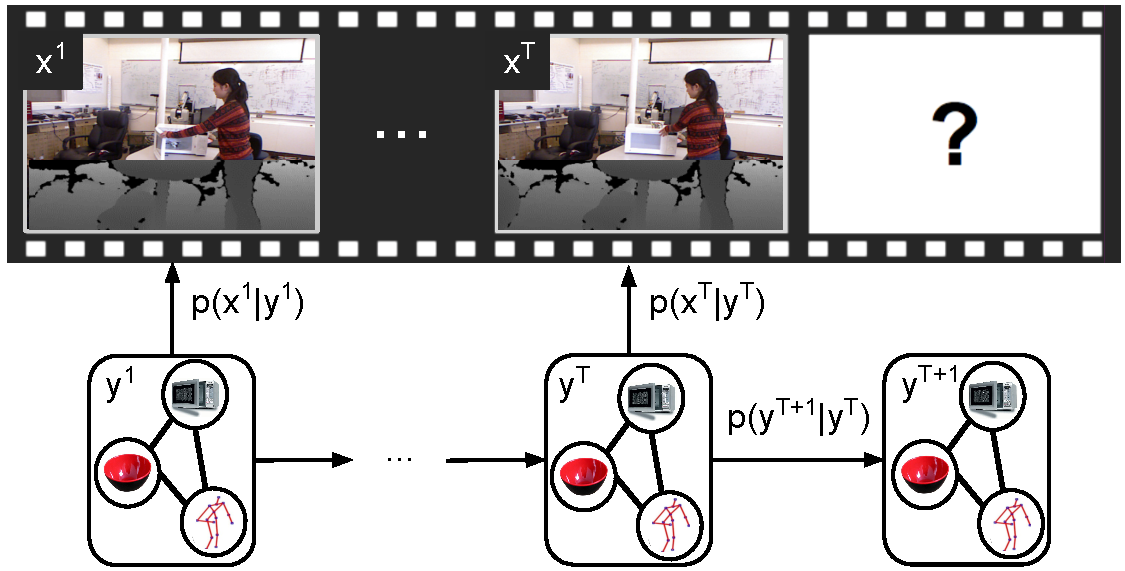
\includegraphics[width=\textwidth]{Fig1}
\caption{Figure is showing the state and measurements at each time represented by a CRF.
Our algorithm, rCRF, enables the application of recursive Bayesian estimation to CRF-based scene models. rCRF computes the full belief over human activity and object affordances ($y^1,\ldots,y^{T+M}$) by using RGB-D Video ($x^1,\ldots,x^T$).}
% In order to so, we propose a new model, rCRF, which can jointly use bayesian filtering and CRFs.}
%  which are not observed.}
%Estimating the belief over a CRF and using the estimated belief for anticipation and robot planning. \emph{(Colors of the nodes are representing the labels.)}}
\label{fig1}
\end{figure}

% modeling temporal evolution is still challenging in such a setting since the sampling procedure does not use temporal information \emph{(see Section~\ref{relwork} for mote details on this challenge)}.
Bayesian filtering methods can accurately estimate a belief (set of probabilities) over variables of interest from sequential data. However, it is still very challenging to estimate a belief over a CRF for two reasons. Firstly, it is not tractable to enumerate the labels over a CRF model since the output space has a dimension exponential in the number of objects, labels, and the temporal length\footnote{Typically with 10 objects, 10 min. length (with 1 sec. long segments), 10 activity and 10 object labels, dimension is $(10^{10}\times10)^{10\times60}=10^{6600}$.}. Secondly, there is a modelling difference between CRFs and Bayesian filtering framework. CRF is based on a discriminative setting whereas the Bayesian filtering mostly relies on the generative formulation.
% that requires the conditional probability of the observation given the variables of interest.
%where it models the conditional probability of the variables of interest given an observation,

In this chapter, we present a recursive algorithm -- Recursive CRF (rCRF) -- which can efficiently estimate a full belief over a CRF-based temporal scene model. rCRF can be seen as an efficient belief estimation method which enables us to use CRF-based scene model in Bayesian filtering. It models the temporal evolution via Bayesian updates and models the measurements in the scene via CRF. In order to use CRFs in such a scenario, we solve two problems. First, we present an approximation to convert the discriminative likelihood of the CRF into a generative measurement equation. Second, we use structured diversity for tractable computation. To the best of our knowledge, rCRF is the only tractable method that can use a CRF-based scene model in a recursive Bayesian filtering.
%Since we define the belief function recursively, we iterate the message propagation and diverse sampling until the convergence.

We apply the rCRF to the problem of activity detection and anticipation from RGB-D data. As a CRF-based scene model, we use the model from \cite{hemaIJRR} which represents the scene as a CRF over human activity and object affordances. We then use the RGB-D video to detect and anticipate activities via rCRF. %We use the rCRF framework in order to anticipate the future activities as well.

Our experiments show that we outperform the state-of-the-art methods for detection and anticipation, and the improvement in the anticipation accuracy is significant. In addition to the improvements in accuracy, we show that our anticipation also improves the computation time and runs near real-time.

%We believe that the presented efficient and accurate estimation of a full belief can be combined with an optimal decision mechanisms (e.g. minimum Bayes risk \cite{decisionTheory,nabbe2007extending}) for better assitive robots.

In summary, the contributions of this work are:
\begin{itemize}
\item  We present Recursive-CRF (rCRF) method that uses the rich modeling power of CRF in
Bayesian filtering setting.
%  allows CRF-based scene models in a Bayesian filtering.
% \item  We present a recursive method in order to estimate the full belief over an rCRF.
\item  We present a structured-diversity based approach to enable tractable computation of the belief.
\item  We apply our rCRF method to the problem of activity detection and anticipation in
RGB-D videos.
%\item  Our experiments show that rCRF significantly outperforms the state-of-the-art methods, both in accuracy and inference time.
\end{itemize}

\input{papers/ijcv/related}
% !TEX root = robobrain.tex

% \section{Technical Challenges}
\section{Overview}
\label{overviewPaper}

\robobrain{} is a never ending learning system  that  continuously incorporates
new knowledge from  its partner projects and from different Internet sources.
One of the functions of \robobrain{} is to represent the knowledge from various sources as a graph,
as shown in  Figure~\ref{fig:graph}. The nodes of the graph represent concepts and edges represent the
relations between them. The connectivity of the graph is increased through a set of graph operations
that allow additions, deletions and updates to the graph. As of the date of this submission,
\robobrain{} has successfully
connected knowledge from sources like WordNet, ImageNet, Freebase, OpenCyc,
 parts of Wikipedia and other partner projects. These knowledge sources provide lexical knowledge, grounding of concepts into images and common sense facts about the world.

The knowledge from the partner projects and Internet sources can sometimes be erroneous. \robobrain{}
handles inaccuracies in  knowledge by maintaining beliefs over the correctness of the concepts and
relations. These beliefs depend on how much \robobrain{} trusts a given source of knowledge, and also the
feedback it receives from crowd-sourcing (described below). For every incoming knowledge, \robobrain{}
also makes a sequence of decisions on whether to form new nodes, or edges, or both. Since the
knowledge carries semantic meaning \robobrain{} makes many of these decisions based on the
contextual information that it gathers from nearby nodes and edges. For example, \robobrain{} resolves
polysemy using the context associated with nodes. Resolving polysemy is important because a `plant'
could mean a `tree' or an `industrial plant' and merging the nodes together will create errors in the
graph.


\robobrain{} incorporates supervisory signals from humans in the form of crowd-sourcing feedback. This
feedback allows \robobrain{} to update its beliefs over the correctness of the knowledge, and to modify the
graph structure if required. While crowd-sourcing feedback was used in some previous works as
means for data collection (e.g.,~\citep{imagenet2009,Russell08}), in \robobrain{} they serve as supervisory
signals that improve the knowledge engine. \robobrain{} allows user interactions at multiple levels: (i)~
Coarse feedback: these are binary feedback where a user can ``Approve'' or ``Disapprove'' a concept
in \robobrain{} through its online web interface; (ii) Graph feedback: these feedback are elicited on 
\robobrain{} \textit{graph visualizer}, where a user modifies the graph by adding/deleting nodes or edges; (iii)
Robot feedback: these are the physical feedback given by users directly on the robot.

In this paper we discuss different aspects of \robobrain{}, and show how \robobrain{} serves as a knowledge layer for the robots. In order to support knowledge sharing, learning, and crowd-sourcing feedback we develop a large-scale distributed system. We describe the architecture of our  system in Section~\ref{sec:system}. In Section~\ref{sec:raquel} we describe the robot query library, which allow robots to interact with \robobrain{}.  Through experiments we show that robots can use \robobrain{} \textit{as-a-service} and that knowledge sharing through \robobrain{} improves existing robotic applications. We now present a formal definition of our Robot Knowledge Engine and the graph.

\input{papers/ijcv/method-features}
\input{papers/ijcv/method-learning}
% !TEX root = rCRF.tex
\section{Experimental Results}
In order to experimentally evaluate the proposed rCRF model and the belief computation, we perform experiments on two applications. Firstly, we estimate a belief over the activity a human is performing and the affordances of the objects in the scene by using the RGB-D video. After computing the belief, we detect the most likely activity and affordance sequences and study the improvement in the detection accuracy. Secondly, we test the accuracy of the beliefs in the anticipation setting. Indeed, we show that it is possible to obtain high-quality detection and anticipation via rCRF.

\begin{figure}[ht]
\small
%\begin{singlespace}
\begin{tabular}{p{5mm}@{}l}
\begin{tabular}{r}
\rotatebox[origin=r]{90}{\;\;\;\;\;\;\;Middle Frame}\\
\rotatebox[origin=l]{90}{Belief\;\;\;\;\;\;\;}
\end{tabular}
&
\begin{tabular}{p{3.7cm}p{3.7cm}p{3.7cm}p{3.7cm}}
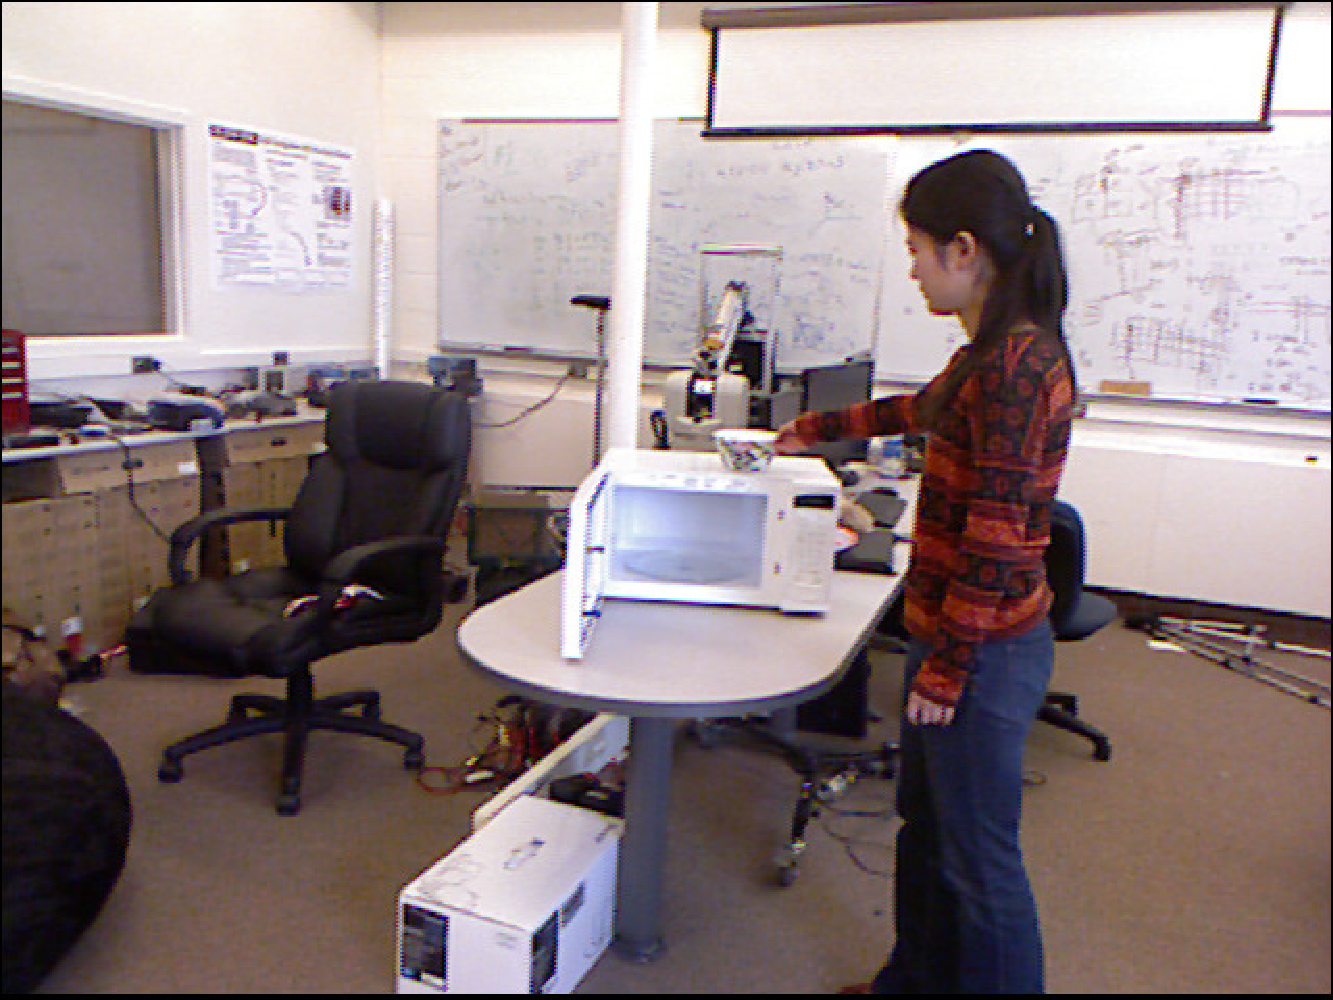
\includegraphics[width=0.225\textwidth]{f10} &
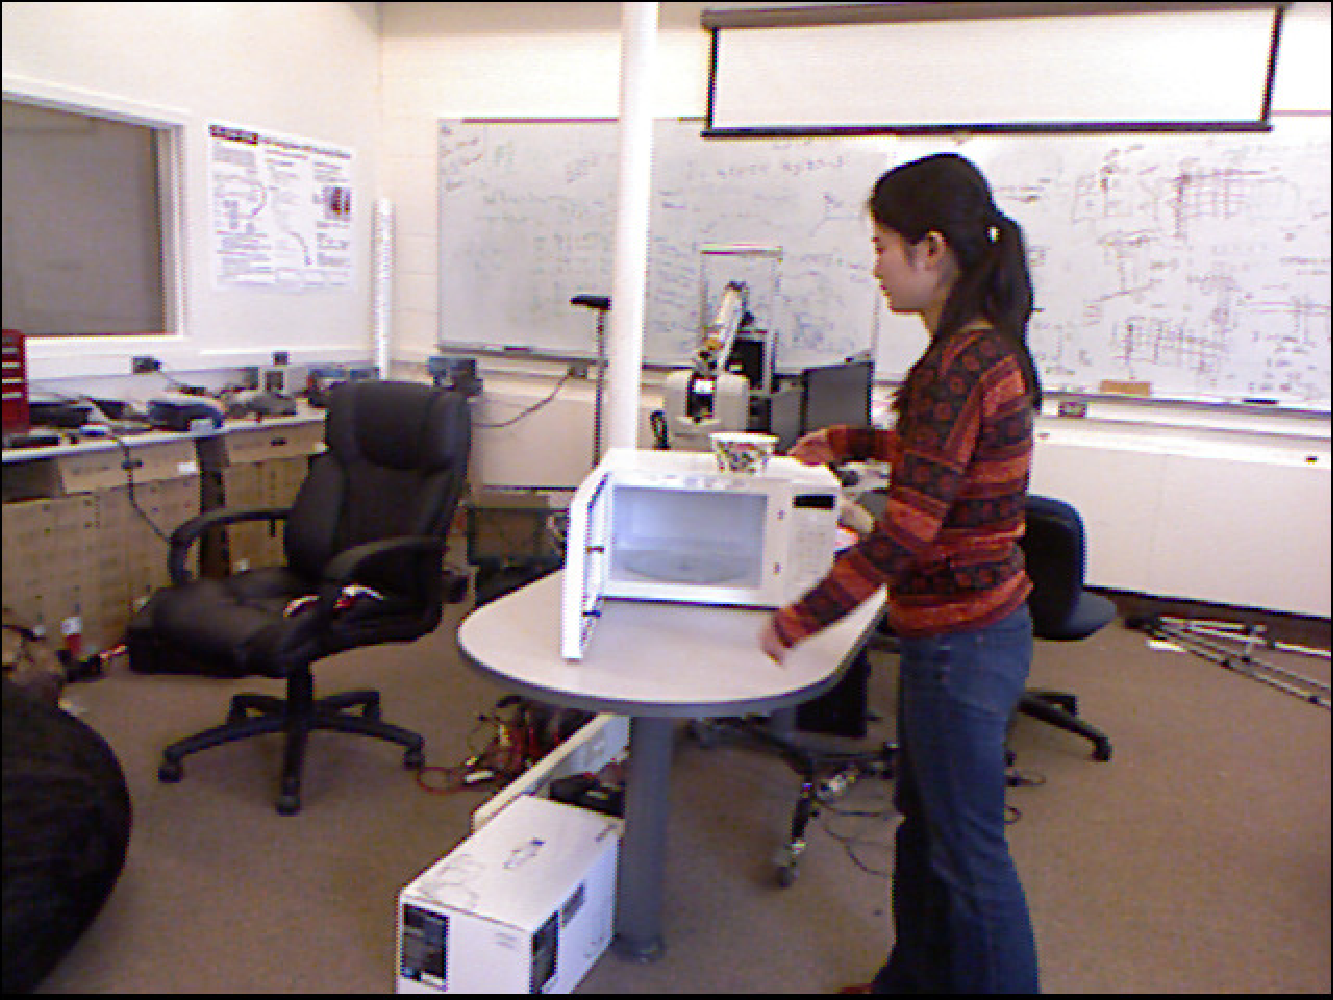
\includegraphics[width=0.225\textwidth]{f11} &
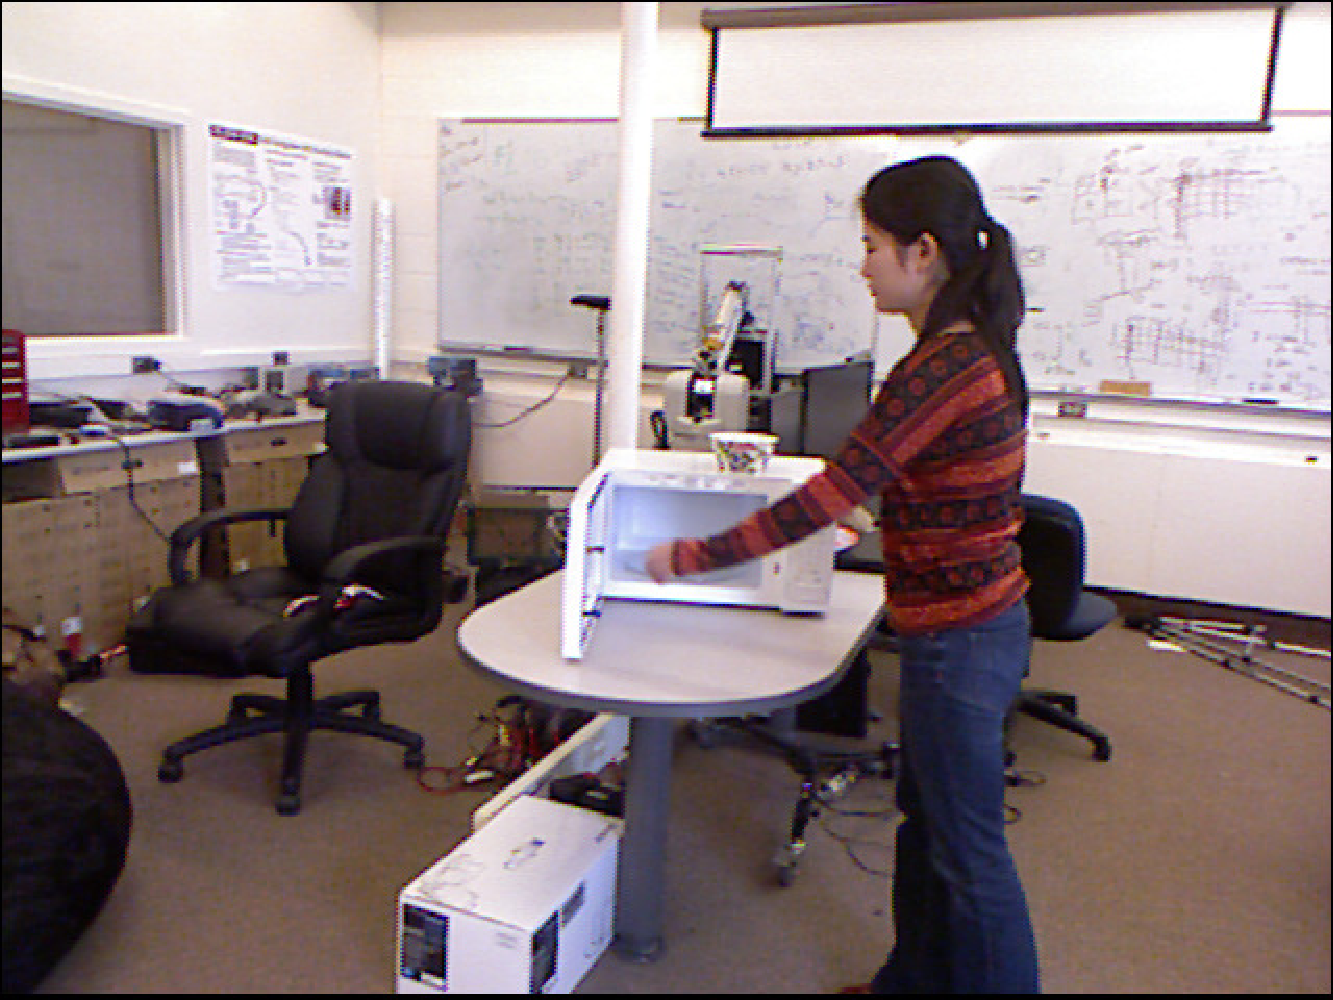
\includegraphics[width=0.225\textwidth]{f12} &
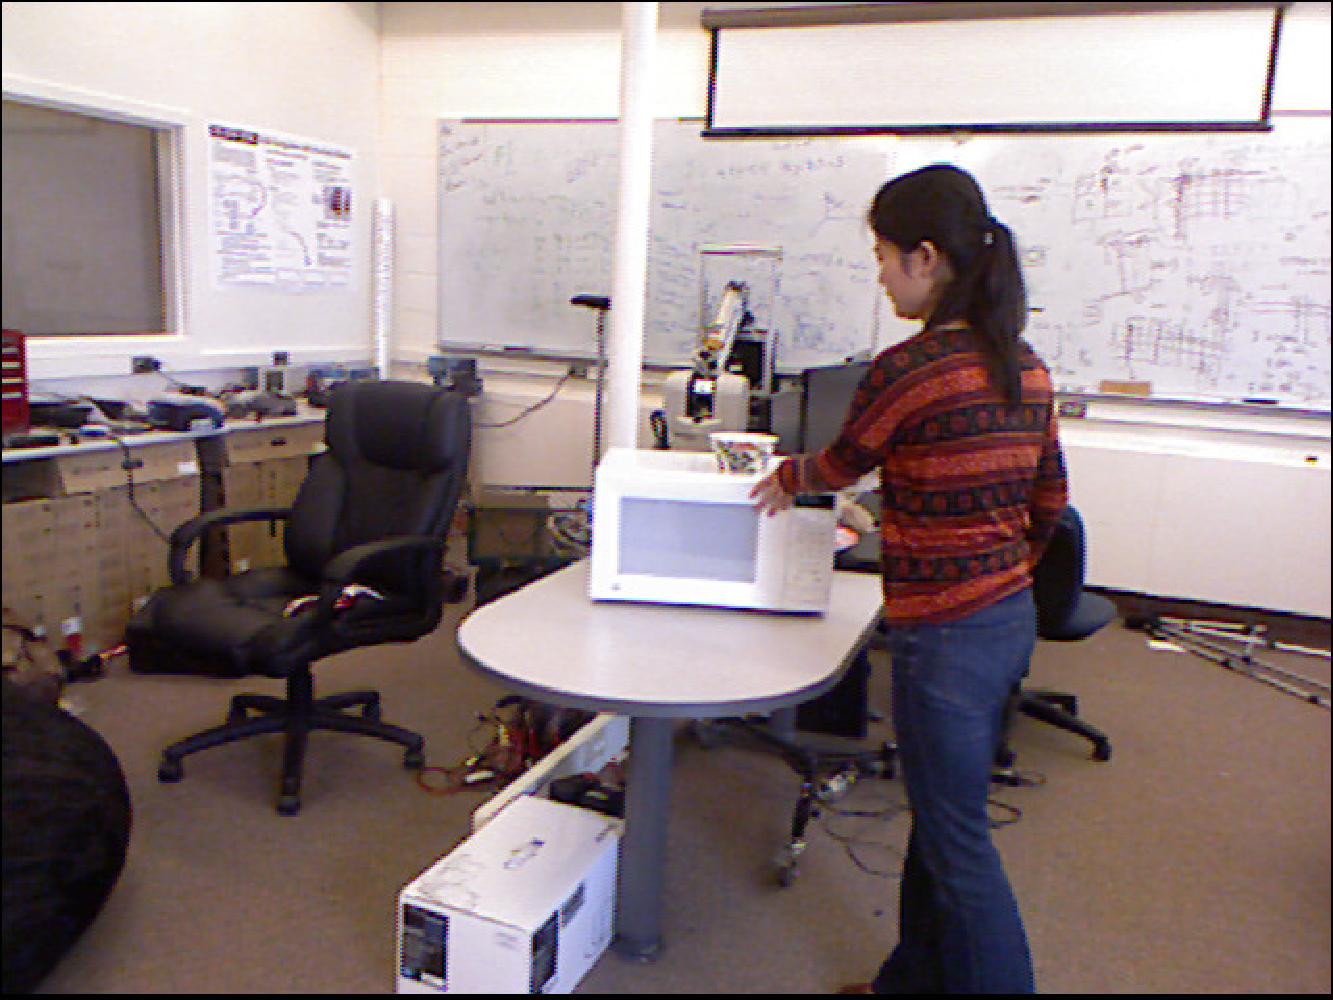
\includegraphics[width=0.225\textwidth]{f13}  \\ %\\%\begin{tabular}{p{3.6cm}p{3.6cm}p{3.6cm}p{3.6cm}}
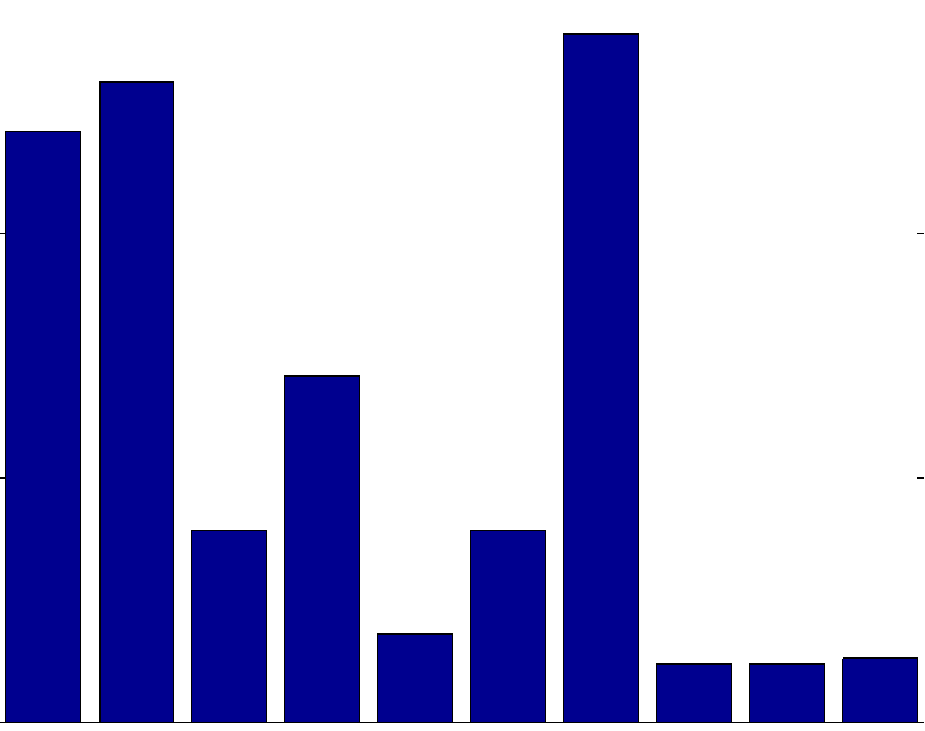
\includegraphics[width=0.225\textwidth, height=8mm]{P10} &
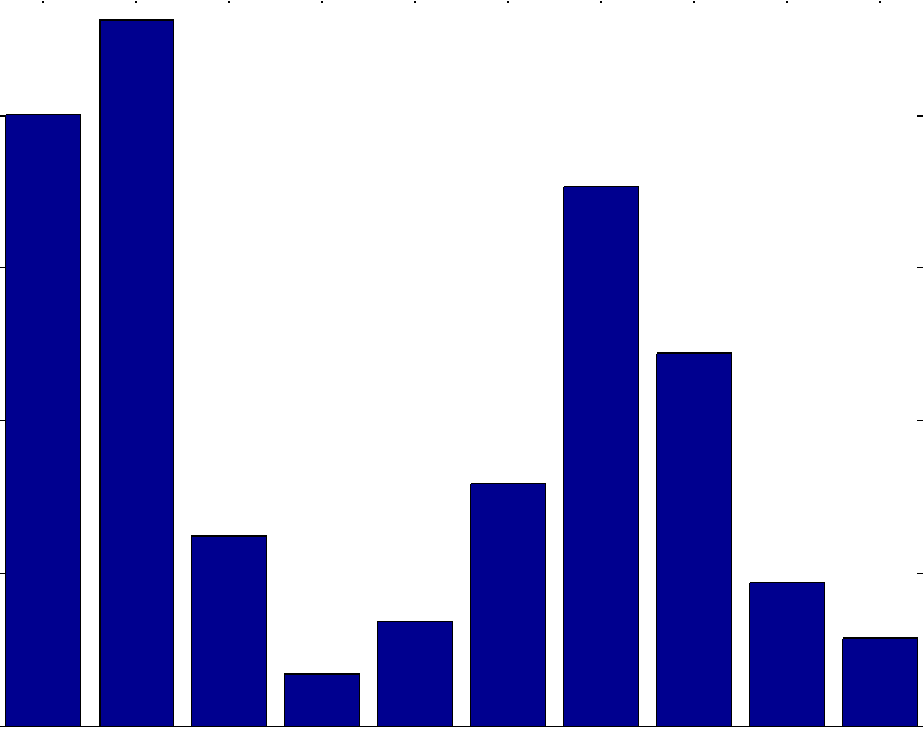
\includegraphics[width=0.225\textwidth, height=8mm]{P12P} &
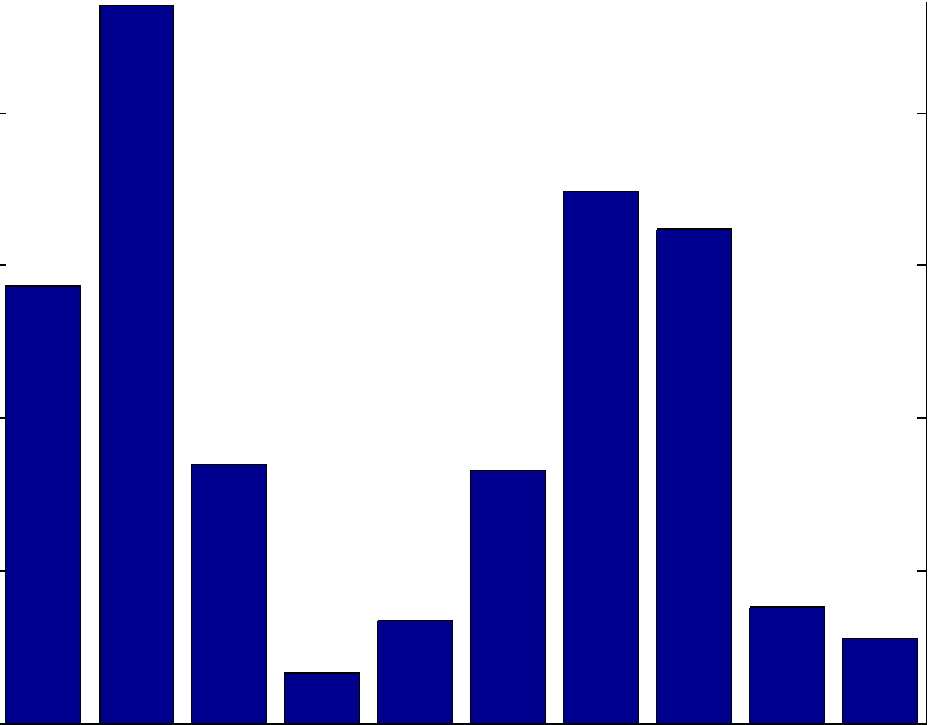
\includegraphics[width=0.225\textwidth, height=8mm]{P13P} &
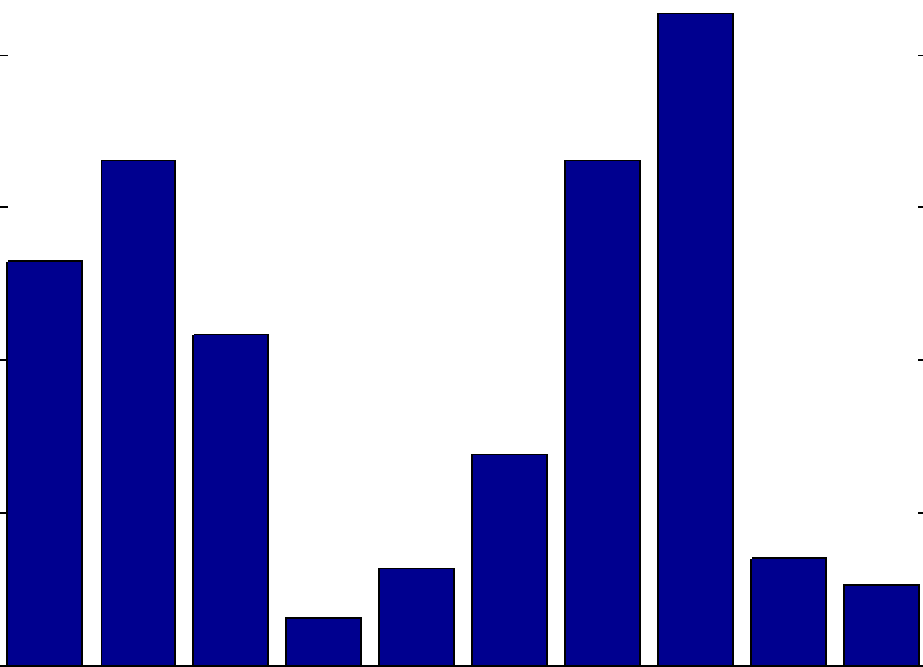
\includegraphics[width=0.225\textwidth, height=8mm]{P14P}  \\

\vspace{-6mm}\hspace{-1mm}\scalebox{0.84}{
\rotatebox[origin=r]{90}{reaching}\hspace{1mm}
\rotatebox[origin=r]{90}{moving}\hspace{1mm}
\rotatebox[origin=r]{90}{pouring}\hspace{1mm}
\rotatebox[origin=r]{90}{eating}\hspace{1mm}
\rotatebox[origin=r]{90}{drinking}\hspace{1mm}
\rotatebox[origin=r]{90}{opening}\hspace{1mm}
\rotatebox[origin=r]{90}{placing}\hspace{1mm}
\rotatebox[origin=r]{90}{closing}\hspace{1mm}
\rotatebox[origin=r]{90}{null}\hspace{1mm}
\rotatebox[origin=r]{90}{cleaning}}&
\vspace{-6mm}\hspace{-1mm}\scalebox{0.84}{
\rotatebox[origin=r]{90}{reaching}\hspace{1mm}
\rotatebox[origin=r]{90}{moving}\hspace{1mm}
\rotatebox[origin=r]{90}{pouring}\hspace{1mm}
\rotatebox[origin=r]{90}{eating}\hspace{1mm}
\rotatebox[origin=r]{90}{drinking}\hspace{1mm}
\rotatebox[origin=r]{90}{opening}\hspace{1mm}
\rotatebox[origin=r]{90}{placing}\hspace{1mm}
\rotatebox[origin=r]{90}{closing}\hspace{1mm}
\rotatebox[origin=r]{90}{null}\hspace{1mm}
\rotatebox[origin=r]{90}{cleaning}}&
\vspace{-6mm}\hspace{-1mm}\scalebox{0.84}{
\rotatebox[origin=r]{90}{reaching}\hspace{1mm}
\rotatebox[origin=r]{90}{moving}\hspace{1mm}
\rotatebox[origin=r]{90}{pouring}\hspace{1mm}
\rotatebox[origin=r]{90}{eating}\hspace{1mm}
\rotatebox[origin=r]{90}{drinking}\hspace{1mm}
\rotatebox[origin=r]{90}{opening}\hspace{1mm}
\rotatebox[origin=r]{90}{placing}\hspace{1mm}
\rotatebox[origin=r]{90}{closing}\hspace{1mm}
\rotatebox[origin=r]{90}{null}\hspace{1mm}
\rotatebox[origin=r]{90}{cleaning}}&
\vspace{-6mm}\hspace{-1mm}\scalebox{0.84}{
\rotatebox[origin=r]{90}{reaching}\hspace{1mm}
\rotatebox[origin=r]{90}{moving}\hspace{1mm}
\rotatebox[origin=r]{90}{pouring}\hspace{1mm}
\rotatebox[origin=r]{90}{eating}\hspace{1mm}
\rotatebox[origin=r]{90}{drinking}\hspace{1mm}
\rotatebox[origin=r]{90}{opening}\hspace{1mm}
\rotatebox[origin=r]{90}{placing}\hspace{1mm}
\rotatebox[origin=r]{90}{closing}\hspace{1mm}
\rotatebox[origin=r]{90}{null}\hspace{1mm}
\rotatebox[origin=r]{90}{cleaning}}
\end{tabular}
\end{tabular}

\begin{tabular}{p{5mm}@{}l}
\begin{tabular}{r}
\rotatebox[origin=r]{90}{\;\;\;\;\;\;\;Middle Frame}\\
\rotatebox[origin=l]{90}{Belief\;\;\;\;\;\;\;}
\end{tabular}
&
\begin{tabular}{p{3.7cm}p{3.7cm}p{3.7cm}p{3.7cm}}
\includegraphics[width=0.225\textwidth]{l5} &
\includegraphics[width=0.225\textwidth]{l6} &
\includegraphics[width=0.225\textwidth]{l7} &
\includegraphics[width=0.225\textwidth]{l8}  \\
\includegraphics[width=0.225\textwidth, height=9mm]{bl5} &
\includegraphics[width=0.225\textwidth, height=9mm]{bl6_2} &
\includegraphics[width=0.225\textwidth, height=9mm]{bl7_2} &
\includegraphics[width=0.225\textwidth, height=9mm]{bl8_2}  \\
\iffalse
\begin{tikzpicture}[remember picture,overlay]
\node[anchor=south west,inner sep=0] (image1)
  {\includegraphics[width=0.22\textwidth, height=10mm]{bl5}};
\end{tikzpicture} &
\begin{tikzpicture}[remember picture,overlay]
\node[anchor=south west,inner sep=0] (image2)
  {\includegraphics[width=0.22\textwidth, height=10mm]{bl6_2}};
\end{tikzpicture} &
\begin{tikzpicture}[remember picture,overlay]
\node[anchor=south west,inner sep=0] (image3)
  {\includegraphics[width=0.22\textwidth, height=10mm]{bl7_2}};
\end{tikzpicture} &
\begin{tikzpicture}[remember picture,overlay]
\node[anchor=south west,inner sep=0] (image4)
  {\includegraphics[width=0.22\textwidth, height=10mm]{bl8_2}};
\end{tikzpicture}
\begin{tikzpicture}[remember picture,overlay]
\draw[->,line width=2pt,red!80!black]
([yshift=-5pt,xshift=14pt]image4.west) |-
([yshift=-5pt,xshift=81pt]image3.west);
\draw[->,line width=2pt,red!80!black]
([yshift=0pt,xshift=81pt]image3.west) |-
([yshift=0pt,xshift=13pt]image2.west);
\draw[->,line width=2pt,red!80!black]
([yshift=-5pt,xshift=13pt]image2.west) |-
([yshift=-5pt,xshift=5pt]image1.west);
\end{tikzpicture}
\fi
\vspace{-6mm}\hspace{-1mm}\scalebox{0.84}{
\rotatebox[origin=r]{90}{reaching}\hspace{1mm}
\rotatebox[origin=r]{90}{moving}\hspace{1mm}
\rotatebox[origin=r]{90}{pouring}\hspace{1mm}
\rotatebox[origin=r]{90}{eating}\hspace{1mm}
\rotatebox[origin=r]{90}{drinking}\hspace{1mm}
\rotatebox[origin=r]{90}{opening}\hspace{1mm}
\rotatebox[origin=r]{90}{placing}\hspace{1mm}
\rotatebox[origin=r]{90}{closing}\hspace{1mm}
\rotatebox[origin=r]{90}{null}\hspace{1mm}
\rotatebox[origin=r]{90}{cleaning}}&
\vspace{-6mm}\hspace{-1mm}\scalebox{0.84}{
\rotatebox[origin=r]{90}{reaching}\hspace{1mm}
\rotatebox[origin=r]{90}{moving}\hspace{1mm}
\rotatebox[origin=r]{90}{pouring}\hspace{1mm}
\rotatebox[origin=r]{90}{eating}\hspace{1mm}
\rotatebox[origin=r]{90}{drinking}\hspace{1mm}
\rotatebox[origin=r]{90}{opening}\hspace{1mm}
\rotatebox[origin=r]{90}{placing}\hspace{1mm}
\rotatebox[origin=r]{90}{closing}\hspace{1mm}
\rotatebox[origin=r]{90}{null}\hspace{1mm}
\rotatebox[origin=r]{90}{cleaning}}&
\vspace{-6mm}\hspace{-1mm}\scalebox{0.84}{
\rotatebox[origin=r]{90}{reaching}\hspace{1mm}
\rotatebox[origin=r]{90}{moving}\hspace{1mm}
\rotatebox[origin=r]{90}{pouring}\hspace{1mm}
\rotatebox[origin=r]{90}{eating}\hspace{1mm}
\rotatebox[origin=r]{90}{drinking}\hspace{1mm}
\rotatebox[origin=r]{90}{opening}\hspace{1mm}
\rotatebox[origin=r]{90}{placing}\hspace{1mm}
\rotatebox[origin=r]{90}{closing}\hspace{1mm}
\rotatebox[origin=r]{90}{null}\hspace{1mm}
\rotatebox[origin=r]{90}{cleaning}}&
\vspace{-6mm}\hspace{-1mm}\scalebox{0.84}{
\rotatebox[origin=r]{90}{reaching}\hspace{1mm}
\rotatebox[origin=r]{90}{moving}\hspace{1mm}
\rotatebox[origin=r]{90}{pouring}\hspace{1mm}
\rotatebox[origin=r]{90}{eating}\hspace{1mm}
\rotatebox[origin=r]{90}{drinking}\hspace{1mm}
\rotatebox[origin=r]{90}{opening}\hspace{1mm}
\rotatebox[origin=r]{90}{placing}\hspace{1mm}
\rotatebox[origin=r]{90}{closing}\hspace{1mm}
\rotatebox[origin=r]{90}{null}\hspace{1mm}
\rotatebox[origin=r]{90}{cleaning}}
\end{tabular}
\end{tabular}
\caption{\textbf{Anticipated belief over activity.} In the first and third row, we show a middle frame of the temporal segment. In the second and fourth row, we show the anticipated belief we computed for the middle frame. Note that frames are not visible to the algorithm and only included for evaluation.}
%\vspace{-4mm}
\label{abcd}
%\end{singlespace}
\end{figure}


\noindent {\bf Data:} We use CAD-120 \cite{hemaIJRR} dataset in order to evaluate our method. CAD-120 dataset includes 120 RGB-D videos of four different subject performing activities \emph{reaching, moving, pouring, etc.} while interacting with objects having affordances \emph{reachable, movable, pourable, etc.}. There are 10 activity classes and 12 object affordance classes.

\noindent {\bf Experimental Setup:} For computing the features and learning the CRF parameters, we follow the approach and the code in \cite{hemaIJRR}. Following the convention in \cite{hemaIJRR}, we use 4-fold cross-validation by training over the data from 3 subjects and testing on the remaining subject. We then average the results over 4-folds. We implemented the rCRF as we explain in Algorithm~\ref{alg:recursive} with the following parameters obtainded via cross-validation; we sampled $M=15$ diverse samples and ran the recursive message updates with the number of iterations limit as $5$.

For the anticipation setting, In order to experiment the $\tau$ seconds into the future anticipation, we experiment over all feasible anticipation scenarios. In other words, we anticipated the time instant $t+\tau$ by using the segments $1\ldots t$ for all $t<T-\tau$, where $T$ is the length of the video. Then, we averaged the score over all feasible experiments.

\noindent {\bf Baseline Algorithms:} In detection setting, we compare the detection results of the rCRF to MAP solution of the spatiotemporal CRF in \cite{hemaIJRR}. We also included the state-of-the art activity detection results from Hu et al. \cite{latentIcra}. Moreover, \cite{latentIcra} is not based on object affordances and it only outputs activity detections. For the anticipation, we compare the rCRF with the state-of-the-art anticipation methods ATCRF \cite{hemaAnt} and GP-LCRF\cite{gpcrf}. We also include DCRF\cite{ddcrf}. In order to evaluate the contribution of the recursive modeling and the structured diversity separately, we also compare the rCRF with a recursive approach without diversity and a diversity-based approach without recursive modeling baselines.

The DivMBest algorithm in \cite{divmbest} uses the diverse sampling method to sample CRFs defined over each frame separately. DivMBest\cite{divmbest} then finds the most likely sequence via Viterbi algorithm. Since it is missing the recursive modeling, it serves as \emph{structured diversity without recursive filtering} baseline. We replace the diversity-based sampling in our method with Gibbs sampler and consider it as \emph{recursive filtering approach without structured diversity} baseline. For the Gibbs sampling, we sampled $50$ samples per temporal segment. We denote the recursive approach with Gibbs sampling as \emph{\mbox{"rCRF w/o div"}} while tabulating the results.

\noindent {\bf Evaluation Metrics:} For activity detection, we compute the ratio of the correctly classified labels (\emph{micro precision}) and the averages of the precision and recall values computed for each activity and object affordance classes (\emph{macro precision} and \emph{macro recall}). For anticipation, we record the ratio of the correctly classified labels \emph{micro precision}, the average of the f-1 score that is computed for each activity and object affordance class (\emph{macro f-1 score}), and the precision of the top 3 anticipated labels (\emph{robot anticipation metric}). While computing the \emph{robot anticipation metric}; if any of the top 3 anticipation is correct, it is counted as true positive.

\noindent {\bf Accuracy of the rCRF in detection setting.}
We evaluate the rCRF for activity detection and summarize the results in Table~\ref{Tdet}. Table~\ref{Tdet} suggests that the rCRF outperforms the MAP solution \cite{hemaIJRR} and performs similarly with the state-of-the-art solution \cite{latentIcra}. Since rCRF and \cite{hemaIJRR} are using the same spatial relations, the performance difference is due to the modeling of the temporal relations in rCRF. We use \mbox{first-order} statistics as temporal dynamics, and they are quite accurate as shown in the heatmap in Figure~\ref{heatmap}. They also capture semantic information like objects become stationary after being used.

\begin{figure}
  \subfigure[Human Activity]{\includegraphics[width=0.48\textwidth]{tranAct}}~
  \subfigure[Object Affordance]{ \includegraphics[width=0.48\textwidth]{tranObj}}
  \caption{Heatmap of the first-order statistics of activity and object affordance classes. They are used as temporal dynamics by rCRF.}
  \label{heatmap}
\end{figure}

\noindent {\bf Accuracy of the rCRF in anticipation setting.}
We evaluate the accuracy of the belief we compute via rCRF, both quantitatively and qualitatively. For qualitative evaluation, we show the segment that we are anticipating the belief over, as well as the belief we obtain in Figure~\ref{abcd}. Please note that, this visual information is not visible to the algorithm, and it is only included for the subjective evaluation.

As shown in the figure, anticipated belief is capturing the scene accurately. Belief is accurate even for the case of concurrent activities. For example, in the second column of the second row in Figure \ref{abcd}, subject is reaching the microwave and moving the cleaner. Our method assigns similar likelihood values to both reaching and moving.

We also perform quantitative analysis over anticipation accuracy. We anticipate 3 seconds into the future and summarize the results in Table~\ref{Tant}. As shown in the Table~\ref{Tant}, rCRF outperforms the state-of-the-art heuristic method \cite{hemaAnt} and the GP-LCRF method \cite{gpcrf} significantly as well as all other baselines. We believe this result is due to the accurate joint-modeling of the temporal relations and the CRF model. We further analysed this behaviour in the subsequent sections.

\begin{table}[ht]
\centering
\tabcolsep=0.7mm
\footnotesize
%\vspace{-1mm}
\caption{\textbf{Detection Performance over CAD-120.}  We compare rCRF with MAP solution and baselines for detections accuracy.}
%\vspace{-1mm}
\begin{tabular}{@{}l@{}|ccc|ccc@{}} \hline
& \multicolumn{3}{@{}|c@{}}{Sub-activity } &   \multicolumn{3}{@{}|c@{}}{Object Affordance } \\ \hline
& micro & \multicolumn{2}{@{}c|@{}}{macro} &   micro & \multicolumn{2}{@{}c@{}}{macro} \\
% \hline
 & prec(\%) & prec(\%) & rec(\%) &   prec(\%) & prec(\%) & rec(\%) \\
\hline
Chance & $10.0${\scriptsize $\pm 0.1$}  & $10.0${\scriptsize $\pm 0.1$}  & $10.0${\scriptsize $\pm 0.1$}  & $8.3${\scriptsize $\pm 0.1$}  & $8.3${\scriptsize $\pm 0.1$}  & $8.3${\scriptsize $\pm 0.1$}  \\
Hu et al.\cite{latentIcra} & $67.8${\scriptsize $\pm 1.4$}  &  $65.5${\scriptsize $\pm 3.5$}&  $\mathbf{63.5}${\scriptsize $\mathbf{\pm 6.6}$}  & N/A & N/A & N/A \\
MAP Sol\cite{hemaIJRR} & $63.4${\scriptsize $\pm 1.6$}  &  $65.3${\scriptsize $\pm 2.3$}&  $54.0${\scriptsize $\pm 4.6$}  & $79.4${\scriptsize $\pm 0.8$} & $62.5${\scriptsize $\pm 5.4$} & $50.2${\scriptsize $\pm 4.9$} \\
DivMBest\cite{divmbest}& $64.0${\scriptsize $\pm 1.3$} & $61.7${\scriptsize $\pm 2.1$} & $56.4${\scriptsize $\pm 2.7$} & $80.1${\scriptsize $\pm 1.0$} & $76.2${\scriptsize $\pm 2.5$} & $53.2${\scriptsize $\pm 3.2$} \\
DCRF\cite{ddcrf}& $61.2${\scriptsize $\pm 2.1$} & $62.8${\scriptsize $\pm 2.8$} & $54.3${\scriptsize $\pm 1.5$} & $71.9${\scriptsize $\pm 2.9$} & $80.6${\scriptsize $\pm 2.4$} & $62.5${\scriptsize $\pm 3.6$} \\
rCRF w/o div& $61.2${\scriptsize $\pm 1.8$} & $64.0${\scriptsize $\pm 1.8$} & $52.7${\scriptsize $\pm 3.8$} & $75.2${\scriptsize $\pm 2.4$} & $79.3${\scriptsize $\pm 3.1$} & $63.7${\scriptsize $\pm 2.9$} \\
rCRF&  $\mathbf{68.1}${\scriptsize$\mathbf{\pm 1.3}$} & $\mathbf{66.1}${\scriptsize $\mathbf{\pm 2.7}$} & $57.2${\scriptsize $\pm 3.9$} & $\mathbf{81.5}${\scriptsize $\mathbf{\pm 1.1}$} & $\mathbf{85.2}${\scriptsize $\mathbf{\pm 2.4}$} & $\mathbf{71.6}${\scriptsize $\mathbf{\pm 3.9}$} \\
\hline
\end{tabular}
%\end{singlespace}
\label{Tdet}
\end{table}
\begin{table}[ht]
\centering
\tabcolsep=0.7mm
\footnotesize
\vspace{-1mm}
\caption{\textbf{Anticipation performance for the anticipating 3 seconds in the future.} We compare rCRF with state-of-the-art anticipation algorithm and baselines for anticipation accuracy.}
\vspace{-1mm}
\begin{tabular}{@{}l@{}|ccc|ccc@{}} \hline
& \multicolumn{3}{@{}|c@{}}{Sub-activity } &   \multicolumn{3}{@{}|c@{}}{Object Affordance } \\ \hline
& micro & macro & robot ant. &  micro & macro & robot ant.   \\
Method & prec(\%) & f1-scr(\%) & metric(\%) & prec(\%) & f1-scr(\%) & metric(\%) \\ \hline
Chance & $10.0${\scriptsize $\pm 0.1$} & $10.0${\scriptsize $\pm 0.1$}  & $30.0${\scriptsize $\pm 0.1$} & $8.3${\scriptsize $\pm 0.1$} & $8.3${\scriptsize $\pm 0.1$}  & $24.9${\scriptsize $\pm 0.1$}  \\
GP-LCRF \cite{gpcrf} & $52.1${\scriptsize $\pm 1.2$} & $43.2${\scriptsize $\pm 1.5$} &  $76.1${\scriptsize $\pm 1.5$}  & $68.1${\scriptsize$\pm 1.0$}  & $44.2${\scriptsize $\pm 1.2$}  & $74.9${\scriptsize $\pm 1.1$}  \\
ATCRF \cite{hemaAnt} & $47.7${\scriptsize $\pm 1.6$} & $37.9${\scriptsize $\pm 2.6$} &  $69.2${\scriptsize $\pm 2.1$}  & $66.1${\scriptsize $\pm 1.9$}  & $36.7 ${\scriptsize $\pm 2.3$}  & $71.3${\scriptsize $\pm 1.7$}  \\
DivMBest\cite{divmbest}& $47.9${\scriptsize $\pm 1.4$} & $43.2${\scriptsize $\pm 3.6$} & $71.5${\scriptsize $\pm 2.7$} & $61.3${\scriptsize $\pm 1.4$} & $56.3 ${\scriptsize $\pm 2.1$} & $73.3${\scriptsize $\pm 0.5$} \\
DCRF\cite{ddcrf}& $48.3${\scriptsize $\pm 2.6$} & $35.4${\scriptsize $\pm 1.8$} & $66.6${\scriptsize $\pm 1.1$} &
$55.2${\scriptsize $\pm 3.1$} & $48.5${\scriptsize $\pm 3.1$} & $71.24${\scriptsize $\pm 2.2$} \\
rCRF w/o div& $49.6${\scriptsize $\pm 2.1$} & $39.7${\scriptsize $\pm 2.6$} & $65.1${\scriptsize $\pm 1.1$} & $56.2${\scriptsize $\pm 1.9$} & $47.4${\scriptsize $\pm 3.1$} & $70.8${\scriptsize $\pm 2.5$} \\
rCRF & $\mathbf{54.3}${\scriptsize $\mathbf{\pm 3.9}$} & $\mathbf{45.8}${\scriptsize $\mathbf{\pm 2.7}$} & $\mathbf{76.5}${\scriptsize $\mathbf{\pm 2.6 }$}  & $\mathbf{78.7}${\scriptsize $\mathbf{\pm 3.4}$} &$\mathbf{74.9}${\scriptsize $\mathbf{\pm 3.8}$} & $\mathbf{82.1}${\scriptsize $\mathbf{\pm 2.9}$} \\
\hline
\end{tabular}
\label{Tant}
\end{table}

\noindent {\bf How important is the recursive modeling?}
DivMBest\cite{divmbest} is the application of the structured diversity without recursive modeling of the Bayesian filtering. In all experiments (Table~\ref{Tdet} and \ref{Tant}), rCRF outperforms the DivMBest \cite{divmbest}. We believe this is because rCRF samples  $p(y^t|x^1,\ldots,x^T)$ instead of $p(y^t|x^t)$ as in the case of \cite{divmbest}. In other words, DivMBest \cite{divmbest} samples without considering temporal relations; on the contrary, we sample the full belief directly.

Moreover, the improvement over the DCRF model shows the important of accurate recursive modeling. DCRF uses the recursive modeling without the proposed conversion of the discrimantive likelihood into generative one and it performs poorly. Hence, the proposed conversion is a necessary step.

We also studied the effect of anticipation horizon. We computed precision of all methods for horizons between 1 and 10 seconds and plotted in Figure~\ref{antHor} and \ref{objHor}. We see significant improvements over longer anticipation time horizons.%\footnote{Since ATCRF \cite{hemaAnt} and GP-LCRF \cite{gpcrf} are using the same method to anticipate the future activities and they only differ in modeling details of humans, they behave similarly versus anticipation time as shown in \cite{gpcrf} and we only included \cite{hemaAnt} in the plot.}
%  and we only included \cite{hemaAnt} in the plot for the sake of clarity.
%We only show the result on object affordance anticipation and rest of the results are included in the supplementary material.

In Figure~\ref{antHor} and \ref{objHor}, accuracy of all algorithms decreases with the increasing horizon. One interesting observation is decrease rate of DivMBest is steeper than others. Since DivMBest misses the recursive nature of the problem, accuracy of the belief it computes is limited; hence, the resulting belief does not stay informative with increasing horizon.

\begin{figure}[ht]
\begin{center}
\includegraphics[width=\textwidth]{entTwo}
\caption{Entropy of the belief vs. time \emph{(uniform dist. has $\approx 3.32$ bit entropy)}}
\label{entRop}
\end{center}
\end{figure}

We further computed the entropy of the belief rCRF computes and plotted its average in Figure~\ref{entRop}. The decrease rate of the accuracy is much smaller than the increase rate of the entropy. In summary, recursive modeling is necessary for an accurate belief estimation and rCRF computes flatter yet still informative beliefs with increasing horizon.

\noindent {\bf How to efficiently cover the output space?}
In order to see the effect of structural diversity on covering the output space, we compare the rCRF with a version of it in which we replace diverse sampling with the Gibbs sampler. As expected, Gibbs sampler only sampled the small region around the posterior and failed to cover the output space. Within all experiments, rCRF outperforms Gibbs sampler baseline. Another interesting observation is, as shown in Figure~\ref{antHor}\&\ref{objHor}, although Gibbs sampler based method performed slightly better than other baselines for short horizon activity anticipation, it performed much worse for object affordance. We believe this is because of the dimensionality. Activity space has dimension $10^{T}$ whereas the object affordance space has dimension $12^{T\cdot M}$ where $T$ is the length of the video and $M$ is the number of objects. Hence, diversity plays bigger role with increasing dimension. Moreover, \cite{hemaAnt} uses the domain knowledge by selectively sampling points around the hand, etc. and it performs better than both baselines with increasing horizon. We believe this result is due to the efficient coverage of the output space with heuristics.

\begin{figure}[t]
  \centering
  \includegraphics[width= \textwidth]{AntO}
\caption{Precision vs. anticipation horizon for object affordance.}
\label{antHor}
\end{figure}

\begin{figure}[h!]
  \centering
  \includegraphics[width=\textwidth]{AntA}
\caption{Precision vs. anticipation horizon for subject activities.}
\label{objHor}
\end{figure}

\noindent {\bf Computationally-efficient inference:}
We evaluated the computational efficiency by computing the average computation time for anticipating 3 second in the future via rCRF and the fastest available anticipation algorithm (the ATCRF\cite{hemaAnt}). Within our experiments, we did not include any pre-processing or feature extraction computation (they are same for all algorithms). Our experiments suggest that the rCRF is faster than \cite{hemaAnt} as shown in Table~\ref{speed}. Hence, rCRF model outperforms the state-of-the-art anticipation algorithm in terms of speed in addition to the accuracy.
\begin{table}[h!]
  \centering
%  \vspace{-2mm}
\caption{Computation time for anticipating 3 seconds in the future excluding pre-processing (\emph{see supplementary material for details}).}
%\vspace{-2mm}
  \begin{tabular}{|cc|cc|}
    \hline
  ATCRF \cite{hemaAnt} \; \; & \; \; 34.1s  \; \;  \; & \; \; \;  rCRF \; \; & \; \;  1.41s \\ \hline
  \end{tabular}
  \vspace{-1mm}
  \label{speed}
\end{table}
%\vspace{-2mm}

\noindent {\bf Can rCRF generalize to RGB data?:}
Since there is no RGB activity dataset with object labels, it is hard to compare our algorithm in the RGB activity analysis setting. Removing the concept of the objet form the graph, makes it a chain-CRF and the inference and learning becomes straightforward. However, we still implement our rCRF over a linear-chain CRF for RGB activity analysis. We based our implementation on MPII cooking activity dataset \cite{mpi_cooking} and use the publicly distributed features from the authors webpage. The shared features are HOG, HOF, dense trajetory features and  MBH \cite{dalal}.


%\begin{table}
\begin{table}
  \caption{Anticipation performance for the anticipating 3 seconds in the future in MPII Cooking Dataset\cite{mpi_cooking}.}
\begin{tabular}{l|ccc} \hline
& micro & macro & macro  \\
Method & prec(\%) & prec(\%) & recall(\%) \\ \hline
Chance & $1.5${\scriptsize $\pm 0.6$} & $1.5${\scriptsize $\pm 0.6$}  & $1.5${\scriptsize $\pm 0.6$}  \\
ATCRF \cite{hemaAnt} & $33.4${\scriptsize $\pm 3.3$} & $52.1${\scriptsize $\pm 4.6$}  & $12.1${\scriptsize $\pm 1.4$}  \\
DivMBest\cite{divmbest} & $34.4${\scriptsize $\pm 2.8$} & $55.3${\scriptsize $\pm 5.0$}  & $14.3${\scriptsize $\pm 1.2$}  \\
rCRF & $\mathbf{37.4}${\scriptsize $\mathbf{\pm 2.9}$} & $\mathbf{63.2}${\scriptsize $\mathbf{\pm 5.5}$}  & $\mathbf{26.1}${\scriptsize $\mathbf{\pm 2.6}$}  \\
\hline
\end{tabular}
\label{Tantmpi}
\end{table}

As shown in the Table~\ref{Tantmpi}, our method outperforms all baselines and competing algorithms. We did not include Gibbs sampling here since the dimension of the activity space is rather low and the experiment over diversity is not informative. We believe this result is due to the accurate handling of temporal information in rCRF and it shows that it generalizes to other modalities.

% !TEX root = rCRF.tex

\section{Conclusions}

In this work, we consider the problem of using rich \mbox{CRF-based} scene models in Bayesian filtering setting. We presented the rCRF model which uses rich modelling power of CRFs in recursive Bayesian filtering. We further developed a computationally-tractable method based on Jensen inequality and structured diversity. We performed extensive experiments that
%  the proposed method against the state-of-the-art methods and various baselines. We 
show rCRF  accurately anticipates the future beliefs over CRFs. We also experimentally demonstrated that the recursive framework significantly improves the accuracy of anticipation. Our rCRF not only resulted in more accurate anticipation but also improved the computation time.   




\chapter{Conclusions}
\epigraph{``Down, down, down. Would the fall never come to an end! I wonder how many miles I've''}{\textit{Lewis Carroll\\ Alice's Adventures in Wonderland}}
We started this dissertations with the question of ``Can we extract structured and physically grounded knowledge from the publicly available information on the web''. Although our answer to this questions is not a definite ``yes'' yet, we showed a very promising direction following a study of knowledge-base creation, representation learning and explicit uncertainty modeling. 

Our first major step was identifying key challenges preventing us, roboticists, from using  existing large-scale knowledge bases. After identifying these challenges, we designed and developed a new knowledge based carefully tailored for robots \emph{www.robobrain.me}. 

Obtaining a large-scaled knowledge, our next step was developing large-scale machine learning algorithms which can learn meaningful representations from the available information. Considering the cost of labelling such a large knowledge base, we designed unsupervised video parsing algorithms. Our proposed algorithm discovered emerging patterns from the videos. It learned objects and their dynamics as well as the activities humans perform.

Learning semantic representations of objects and activities from large-scale collection of videos, resulted in an ambitious question. ``Can we go from instructional videos to physical robot plans?''. Main rationale behind asking this question was the availability of very large collections of instructional videos in YouTube. For example, there are 200 thousand videos only to describe \emph{how to make a poached egg?}. Such an end-to-end system requires solving the domain shift between planning knowledge and perception knowledge. Moreover, we proposed a domain adaptation algorithm for this purpose and showed a successful robot plans generated completely from large-scale data with no human supervision.

Our final step was handling the common challenge of all data-driven systems, unknowns. Since none of the knowledge-bases are complete, all data-driven systems will eventually face an environment they never saw. We believe the key to handle this is explicitly modeling uncertainty. We proposed an estimation algorithm to explicitly model uncertainty. 

Using all these methods, we showed a successful demonstrations of robots directly going from unsupervised large-scale data to physically plausible plans in collaboration with humans. Our demonstrations showed a promising direction but we believe there is still a long way to go. In the rest of this section, we discuss the next steps in this ambitious aim.

One big challenge is natural language processing. Within the scope of this thesis, we used very primitive algorithms to parse and understand natural language. We even used a limited human supervision in some of the applications. We believe it is possible to develop very expressive natural language representations for robotics. The key difference to existing natural language processing methods is the representations need to be multi-domain. For example, the representation to ``Cup'' not only include its language properties but also physical and visual properties. In other words, we need joint representations of the words to be used in robotics.

Yet another challenge is the necessity to model common-sense. We all know that butter is most likely to be found in the fridge and screwdriver is probably in the garage. However, we never explicitly mention these kind of knowledge neither in our written text nor in our instructional videos. Hence, we need algorithms which can learn these common-sense concepts. We believe the path to learning common-sense knowledge is following the way babies learn. Babies learn all these concepts by constantly watching adults and also physically playing with them. Hence, we hypothesize this is possible by personal robots constantly gathering information from our houses and sharing with them. Sharing is a key here since it is not tractable for a single robot to learn the entire human common-sense in a tractable amount of time. 

In summary, we studied the problem of robot perception in this dissertation with a focus on large-scale learning approaches. We showed that large-scale data is extremely useful for robots as long as it satisfy a few properties like being multi-modal, multi-domains and physically grounded. We further showed that visual data have strong structural priors like structural diversity, consistency and hierarchy. We developed unsupervised and multi-domain machine learning algorithms using this priors resulting in state-of-the-art performance in many robot perception tasks. After all, we believe we will be able to answer the aforementioned question with a definite ``yes'' as long as we continue to exploit the structure and share the representations.



\appendix
\chapter{Non-Parametric Bayesian}
Appendix chapter 1 text goes here

\chapter{Discrete Optimization Methods Used in the Thesis}
\section{Quadratic Pseudo-Boolean Optimization}
\section{Mixed Integer Programming}


\bibliography{ozan_sener_thesis, references, shortstrings}

\end{document}
